	% ================================================================
% BACHELOR THESIS
% ================================================================

% ----------------------------------------------------------------
% ENVIRONMENT
% ----------------------------------------------------------------

% --- use KOMAScript european classes

\documentclass[enabledeprecatedfontcommands, a4paper,11pt,headsepline,oneside,openany]{scrbook}

% --- import declarations

\usepackage[utf8]{inputenc}

\usepackage{microtype}
\usepackage[ngerman]{babel}
\usepackage{newcent}
\usepackage{graphicx}
\usepackage{parskip}
\usepackage{setspace}
\usepackage{url}
%\PassOptionsToPackage{hyphens}{url}\usepackage{hyperref}
\usepackage{quotmark}
\usepackage{nameref}
\usepackage{hyphenat}
\usepackage[shortcuts]{extdash}
\usepackage{footnote}


\usepackage{natbib}



%\usepackag BachelorThesis.pdfe[longnamesfirst]{natbib}

%%% Packages für APA-Zitierung %%%
%\usepackage[natbibapa]{apacite}
%\usepackage{apalike}


%\usepackage{apacitepp} --> hat fehler verursacht!!!
\usepackage{booktabs}
\usepackage{tabularx}  % damit zellen den rest des zur vergüfung stehenden Platzes teilen




\usepackage[pdftex]{thumbpdf}     % run: thumbpdf
%\usepackage{xcolor}
\usepackage{color}
\usepackage{colortbl}
\usepackage{tabu} 
\usepackage{syntax}
\usepackage{booktabs}
\usepackage{float}
\usepackage[section]{placeins}
\usepackage{listingsutf8}
\usepackage[T1]{fontenc} % für Umlaute in Tabellen caption und label
\usepackage[table]{xcolor}

\usepackage{pdflscape}
\usepackage{geometry}

\lstset{frame=tb,
	language=Python,
	aboveskip=3mm,
	belowskip=3mm,
	showstringspaces=false,
	columns=flexible,
	basicstyle={\small\ttfamily},
	numbers=none,
	numberstyle=\tiny\color{gray},
	keywordstyle=\color{blue},
	commentstyle=\color{dkgreen},
	stringstyle=\color{mauve},
	breaklines=true,
	breakatwhitespace=true,
	tabsize=3,
	literate={ö}{{\"o}}1
			 {ä}{{\"a}}1
			 {ü}{{\"u}}1
			 {Ä}{{\"A}}1
			 {Ö}{{\"O}}1
			 {Ü}{{\"U}}1
}


\usepackage[
    pdfpagemode={UseOutlines},
    pdftitle={Mueller-Dominique_-BT},
    pdfauthor={Dominique, Müller},
    pdfsubject={Automatische Analyse von Kamerabildern zur Prognose des Geburtszeitpunkts von Kälbern},
    pdfkeywords={Smart Farming, OpenCV, Pattern Recognition, Domain Analysis},
    pdfcreator={pdflatex},
    pdfproducer={LaTeX with hyperref},
    colorlinks,
    linkcolor={red!50!black},
    citecolor={red!50!black},
    urlcolor={red!50!black},
    anchorcolor={red!50!black},
    bookmarks=true,
    bookmarksnumbered=true,
    bookmarksopen=true,
    ]{hyperref}
\usepackage{breakurl}



\usepackage{graphicx}
\usepackage{titletoc}
\usepackage{amssymb}% http://ctan.org/pkg/amssymb
\usepackage{pifont}% http://ctan.org/pkg/pifont

\definecolor{maroon}{cmyk}{0,0.87,0.68,0.32}
\definecolor{darkmaroon}{cmyk}{0,0.87,0.68,0.5}

% für Mengenalgebra
\usepackage{amsmath}
\usepackage{amssymb}
\usepackage{textcomp}
\usepackage{gensymb}
% --- display entries in table of contents up to level 5
\newcommand{\xmark}{\ding{55}}%

\setcounter{tocdepth}{2}
\setcounter{secnumdepth}{5}

% --- physical parameters

\onehalfspacing
\pdfadjustspacing=1
\clubpenalty=4500 %
\widowpenalty=10000 %

% change table numbering 
\usepackage{chngcntr}

\usepackage{chngcntr}
\counterwithout{figure}{chapter}
\counterwithout{table}{chapter}
\counterwithout{equation}{chapter}


%----------------------------------------------------------------
% BODY ----------------------------------------------------------------

\begin{document}

\frontmatter
    % ================================================================
% TITLE PAGE
% ================================================================

\begin{titlepage}
	
	\begin{center}

		\small{\hspace{2cm}Berner Fachhochschule\\
			\hspace{2cm}Fachbereich Wirtschaft\\}
		
		\vspace{0.75cm}
		\large{\hspace{2cm}\textrm{Bachelor Thesis }}
		\vspace{0.75cm}
		
		\Huge{\hspace{2cm} Automatische Analyse von Kamerabildern zur Prognose des Geburtszeitpunkts von Kälbern\\}
		
		\vspace{1cm}
		\LARGE{\hspace{2cm}Identifikation von merkmalsbezogenen Schwellwerten und  Anwendung erprobter Softwarebibliotheken zwecks automatischer Analyse von Bildern bei der Geburt von Kälbern   \\
		\vspace{1.75cm}	
			
			
			\LARGE{\hspace{2cm}Dominique Müller}\\
			\vspace{1cm}
			\large{\hspace{2cm}Studiengang Wirtschaftsinformatik\\
				\hspace{2cm}Matrikelnummer 17-263-625}
			
			\vspace{1cm}
			\large\hspace{2cm}Erstgutachter: Prof. Dr. Patrizio Collovà\\
			\large\hspace{2cm}Zweitgutachter: Dr. Klaus-Georg Deck\\}
			\vspace{1cm}
			
			\hspace{2cm} \large{Bern, xx. April 2020} \\

		
		
	\end{center}
	
\end{titlepage}

% ================================================================
% TITLE PAGE
% ================================================================

    % ================================================================
% Management Summary
% ================================================================


\chapter{Management Summary}


    \tableofcontents

\mainmatter
  
	% ================================================================
% CHAPTER 1: Ausgangslage
% ================================================================


\chapter{Ausgangslage}

\section{Beschreibung der Situation }

In den letzten Jahren ist die Landwirtschaft zunehmend unter Druck geraten. Der Primärsektor verliert an volkswirtschaftlicher Bedeutung \cite[S. 1  f.]{Hofer}. Sowohl der Anteil an Beschäftigten als auch die landwirtschaftliche Nutzfläche sinkt \citep[S. 2 ]{Hofer} und Preise für Agrarprodukte sind stark unter Druck \citep[S. 11 ]{Hofer}. Daraus entsteht ein tiefgreifender Strukturwandel \cite[S. 11  f.]{Hofer}. Zahlreiche Landwirte gehen Nebentätigkeiten nach, um zusätzliches Einkommen zu generieren \citep[S. 6]{Hofer}. Deshalb stellen sowohl die Maximierung des landwirtschaftlichen Einkommens als auch die Ermöglichung der Nutzung von Nebenerwerbsquellen besondere Herausforderungen in der Landwirtschaft dar \citep[S. 8]{Stefan2003}. Für selbstständige Landwirte ist es nicht einfach, einem Nebenerwerb nachzugehen.


Auch der Landwirt Peter Müller geht einer Nebenerwerbstätigkeit nach und will daher im landwirtschaftlichen Betrieb\footnote{Standort des Betriebs: Schwellibach 50, CH-1714 Heitenried, Kanton Freiburg} nach innovativen Lösungen suchen, welche der Doppelbelastung entgegenwirken \citep{Muller2019}. \\


\begin{figure}[H]
	\center
	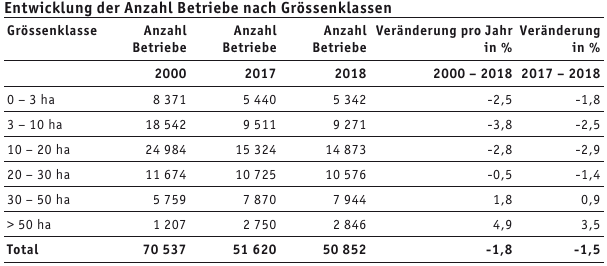
\includegraphics[scale=0.72]{Grafiken/Betriebsstatistik.PNG}
	\caption{Entwicklung der Anzahl Haupt- und Nebenerwerbsbetriebe nach Regionen \citep{Unbekannta}} 
	\label{fig: Entwicklung der Anzahl Haupt- und Nebenerwerbsbetriebe nach Regionen}
\end{figure}


Um möglichst viel Milch zu produzieren, sorgen Landwirte dafür, dass jede Kuh auf dem Bauernhof einmal pro Jahr ein Kalb gebärt. Bei 15 Kühen auf dem Bauernhof des Arbeitgebers, bedeutet dies mehr als eine Geburt pro Monat \citep{Muller2019}.

Jede Geburt, bei welcher der Landwirt abwesend ist, könnte  für die Kuh und das Kalb ein lebensbedrohliches Risiko darstellen \citep{Muller2019}. 

Dieser Bezug zur Problemstellung hat der Autor im Rahmen der Case-Arbeit \flqq{}Technologische Unterstützung von Landwirten bei der Geburt von Kälbern und bei der Heuernte\frqq{} erarbeitet. Es wurde ein System entwickelt, welches in regelmässigen zeitlichen Abständen Kamerabilder aufnimmt und auf einer Website darstellt. Das System zeigt Kamerabilder in passender Qualität zwecks Beobachtung auf einer Website an. Ziel dieses Systems ist eine automatische Unterstützung mit Benachrichtigung auf verschiedenen Kommunikationskanälen bei der Überwachung der Geburt von Kälbern und bei der Heuernte. Weiter soll dadurch das Risiko bei der Geburt von Kälbern und das Risiko von Schäden an der Infrastruktur zur Heuernte reduziert werden.

Sowohl Dr. med. vet. Samuel Kohler, Tierarzt und Studiengangsleiter Agronomie bei der BFH (HAFL) und Prof. Dr. med. vet. Gaby Hirsbrunner vom Departement für klinische Veterinärmedizin der Universität Bern als auch der Auftraggeber, der Landwirt Peter Müller, sehen die Case-Arbeit als spannende Lösung mit Optimierungspotential. Zurzeit müssen die aufgenommenen Kamerabilder von Landwirten nach wie vor auf einer Website angezeigt und von Menschen interpretiert werden. Die computergetriebene, vollautomatische Verarbeitung und Analyse von Kamerabildern stellt eine sinnvolle Weiterentwicklung zur Reduzierung des Überwachungsaufwands dar. 

\section{Bedarf}

Dystokie ist die Todesursache von 50 bis 66\% der Kalbsgeburten mit tödlichem Ausmass. Dies hat auch wirtschaftliche Konsequenzen in Form von Kosten für die Dienstleistungen des Tierarztes, nicht verkauften Kälbern, tieferer Milchproduktion oder vorzeitiger Schlachtung. Darüber hinaus ist Dystokie schmerzvoll und beeinträchtigt das Wohlergehen der Kühe \citep[S. 1]{Saint-Dizier2015}. Die Geburt ist ein kritisches Ereignis für Kuh und Kalb und oftmals Auslöser für nachfolgende Krankheiten. Optimales Management und Überwachung der Geburt wirken diesen Risiken entgegen und vermindern die Eintrittswahrscheinlichkeit von Dystokie und Totgeburt \citep[S. 1]{Lange2017}. Die Prognose des Geburtszeitpunkts unterstützt die Entscheidung, ob und wann menschliche Geburtshilfe angebracht ist. Die Unterstützung beim Abkalben bewirkt eine Verringerung der Kälbersterblichkeit und der Plazenta-Retention. Zusammenfassend ist die Vorhersage des Geburtszeitpunkts daher sowohl für die Wirtschaftlichkeit der Tierhaltung als auch für das Wohlergehen der Tiere von Bedeutung \citep[S. 1]{Saint-Dizier2015}.  


Zum heutigen Zeitpunkt gibt es diverse Lösungsansätze zur Analyse des Geburtsverlaufs. Neigungs- und Beschleunigungssensoren sollen die Schwanzhebung und Verhaltensänderungen erkennen \citep[S. 6]{Saint-Dizier2015}. Zudem können spezialisierte Wiederkäuersensoren, welche beispielsweise von der Forschungsanstalt Agroscope\footnote{Weitere Informationen zu Agroscope: \url{https://www.agroscope.admin.ch}} entwickelt werden, das Wiederkäuerverhalten der Tiere analysieren \citep[S. 2]{Pahl2014}. Intelligente Bauchgürtel sind gemäss \citep[S. 6]{Saint-Dizier2015} in der Lage, Abdominalkontraktionen zu detektieren. Intravaginale Sensoren erkennen einen Abfall der Körpertemperatur und die Ausstossung des Allantochorions. Zudem gibt es Vorrichtungen in der Vagina oder an den Schamlippen, welche die Ausstossung der Waden erkennen. Sämtliche Produkte funktionieren nach demselben Prinzip: Sobald ein Sensor das prädiktive Merkmal erkennt, wird dieses analysiert und eine Benachrichtigung an den Landwirten ausgelöst. So wird der Landwirt vor dem bevorstehenden Abkalben gewarnt. Die wissenschaftliche  Basis der angebotenen Produkte ist  jedoch oftmals mangelhaft. Diese Einschätzung von \citep[S. 6]{Saint-Dizier2015} hat mehrere Ursachen. Einerseits berücksichtigen die Produkte oftmals nur eine geringe Anzahl von Parametern zur Analyse. Andererseits bringt zurzeit keines der getesteten Geräte die Möglichkeit, Dystokie oder die Notwendigkeit menschlicher Geburtsunterstützung zu erkennen. Ausserdem wurden die meisten Studien bei der Rasse Holstein\footnote{ \url{https://www.swissherdbook.ch/unsere-rassen/holstein-red-holstein/}}\textsuperscript{,}\footnote{\url{https://swissgenetics.com/genetik/rassenspezifische-informationen/holstein/}} in Milchkuhhaltung durchgeführt. Sowohl in der Sammlung von Erfahrung bei anderen Rassen als auch anderer Haltung liegt grosses Verbesserungspotential. Dementsprechend ist die Einführung von technischen Systemen zur Sammlung von Daten bei einer grossen Anzahl von Tieren anstrebenswert. So können weitere Wissenquellen gewonnen werden, welche für die Entwicklung von erfolgreicheren Produkten nützlich sind \citep[S. 6]{Saint-Dizier2015}. Die vorliegende Arbeit beinhaltet die Analyse von Kamerabildern während der Geburt von Kälbern der Rasse Swiss Fleckvieh\footnote{\url{https://swissgenetics.com/genetik/rassenspezifische-informationen/swiss-fleckvieh/}}\textsuperscript{,}\footnote{\url{https://www.swissherdbook.ch/unsere-rassen/swiss-fleckvieh/}}. Dadurch kann die Arbeit einen Beitrag zum Gewinn von weiterer Erfahrung in dieser Domäne leisten.

In der Studie von \cite[S. 6]{Ouellet2016} wurden 42 Kühe mit Sensoren ausgestattet, wobei acht davon die Sensoren verloren haben und durch technische Probleme mit dem Wiederkäuersensor bei zwei weiteren Kühen keine Daten zum Wiederkäuerverhalten gesammelt werden konnten. Der Einsatz von Kameras hingegen ermöglicht eine sichere Entfernung zwischen Kuh und technischer Einrichtung. Der Autor ist der Meinung, dass diese Entfernung die Ausfallsicherheit des System erhöhen kann. Um den optimalen Abstand zwischen Kamera und Tieren festzulegen, wurden die empirischen Versuche durch Angaben der Tierärzten überprüft und dementsprechend angepasst.
 
\section{Ziele }

Wünschenswert ist nun, im Rahmen der Bachelor-Thesis ein System zu entwickeln, welches die automatische Analyse von Kamerabildern zur Prognose des Geburtszeitpunkts von Kälbern ermöglicht.

Der Aufwand für die Überwachung des Geburtsverlaufs ist auf ein Minimum reduziert, weil die Lösung vollständig digitalisiert ist.

Dieses System soll modular und erweiterbar sein und optimalerweise auch in der Lage sein, Landwirte und Tierärzte mittels direkter und gezielter Benachrichtigungen fast in Echtzeit über den Geburtsverlauf von Kälbern zu informieren. Grundlage für diese Benachrichtigung bildet die computergetriebene Analyse von Bildmaterial.

Im Rahmen der vorliegenden Bachelor-Thesis wird zwischen Projektzielen (A), betrieblichen (B) und optionalem Zielen (C) unterschieden.


\textbf{Projektziele (Ziele zum Lieferergebnis)}

\begin{table} [H]
	
	\rowcolors{2}{maroon!10}{white!100}
	\arrayrulecolor{darkmaroon} 
	
	\begin{tabular}{ p{1cm} p{14cm} }
				
		\toprule[1pt]
		\rowcolor{maroon!30}	
		ID & Beschreibung \\
		
		\midrule 
		A1 & Das System liest Bilddateien von einem Dateisystem ein.\\		
		A2 & Das System bearbeitet die von der Kamera gelieferten Bilder.\\				
		A3 & Das System arbeitet auf Basis von Mustern und visuellen Merkmalen unter Berücksichtigung gegebener Schwellwerte. \\		
		A4 & Das System arbeitet aus Entfernung zu den Tieren, sodass es sicherer ist.\\				
		A5 & Das System ist durch fundiertes Software-Engineering so aufzubauen,
		dass eine beliebige technische Komponente ausgetauscht werden kann und die
		neue Implementierung für die restlichen Schichten keine Auswirkung hat.\\		
		
		\bottomrule
	\end{tabular}
	\caption{Projektziele}
	\label{tab: Projektziele}
\end{table}

\newpage

\textbf{Ziele im Betrieb}


Die folgende Tabelle verdeutlicht die betrieblichen Ziele im Zusammenhang mit der Geburt von Kälbern.

\begin{table}[H]
	\rowcolors{2}{maroon!10}{white!100}
	\arrayrulecolor{darkmaroon} 
	
	\begin{tabular}{ p{1cm} p{14cm} }
		
		\toprule[1pt]
		\rowcolor{maroon!30}	
		ID & Beschreibung \\
		
		\midrule 
		B1 & Das System reduziert den Aufwand für die manuelle Überwachung des Geburtsverlaufs dank Kamerabildern. \\
		B2 & Das System stellt sowohl für Landwirte als auch Tierärzte ein digitales Werkzeug zur Entscheidungsunterstützung zur Verfügung.\\
		B3 & Das System senkt Geburtsrisiken für Kuh und Kalb. Dies erhöht die Wirtschaftlichkeit der Tierhaltung und das Wohlergehen der Tiere. \\
		B4 & Das System vereinfacht die Einleitung von gezielten Massnahmen zur Geburtshilfe.\\
		\bottomrule
		
	\end{tabular}
	\caption{Betriebliche Ziele für die Überwachung bei der Geburt von Kälbern.}
	\label{tab: Betriebliche Ziele für die Überwachung bei der Geburt von Kälbern.}
\end{table}

\textbf{Optionale Ziele }

Folgende Tabelle verdeutlicht die anstrebenswerten Ziele, welche einen zusätzlichen Mehrwert erschaffen sollen.
\begin{table}[H]
	\rowcolors{2}{maroon!10}{white!100}
	\arrayrulecolor{darkmaroon} 
	
	\begin{tabular}{ p{1cm} p{14cm}  }
		
		\toprule[1pt]
		\rowcolor{maroon!30}		
		
		ID & Beschreibung \\
		
		\midrule 
		C1 & Das System erkennt Bilder bei welchen in den nächsten 12 Stunden noch keine Geburt stattfindet und löst daraufhin eine vordefinierte, konfigurierbare Aktion aus. In einer ersten Phase handelt es sich um eine konfigurierbare Meldung, die in der Konsole der Entwicklungsumgebung ausgegeben wird.\\ 
		C2 & Das System ist in der Lage, Landwirte und Tierärzte mittels Benachrichtigungen als Nachricht über Kommunikationskanäle wie ) SMS, b) Twitter, c) WhatsApp oder d) Mail über den Geburtsverlauf von Kälbern zu informieren.  \\
		\bottomrule
		
	\end{tabular}
	\caption{Optionale Ziele für die Überwachung bei der Geburt von Kälbern.}
	\label{tab: Optionale Ziele für die Überwachung bei der Geburt von Kälbern.}
\end{table}

	% ================================================================
% CHAPTER 2: Methodisches Vorgehen 
% ================================================================
\chapter{Methodisches Vorgehen}

Wie auch in der Case-Arbeit nimmt in der Anfangsphase der Bachelor-Thesis die Business Analyse eine Schlüsselrolle ein. Für die Untersuchung und Wissensgewinnung stellen sowohl per Videotelefonie durchgeführte qualitative Interviews mit Fachleuten (Veterinäre, Landwirte) als auch Literaturrecherchen die wichtigsten Methoden dar. In diesem Rahmen sind zur Gewinnung von Expertenwissen die wesentlichen Merkmale eines Bildes zu identifizieren, welche für Prognose und computergetriebene Analyse des Geburtsverlaufs von Kälbern von Bedeutung sind.  Weiterhin müssen im Rahmen dieser Analyse merkmalsbezogene Muster und Schwellwerte festgelegt werden, die auf eine Geburt eines Kalbes hinweisen. Diese bestimmen, ob und zu welchem Zeitpunkt Landwirte bzw. Tierärzte über den Geburtsverlauf eines Kalbs informiert werden sollen. 

Zudem werden erworbene Kenntnisse aus der Vertiefungsrichtung Business Analyse\footnote{Weitere Informationen: \url{https://moodle.bfh.ch/course/view.php?id=20247}} aus dem Studiengang Wirtschaftsinformatik der Berner Fachhochschule angewendet.  Die im Rahmen der Business Analyse gewonnen Erkenntnisse werden mithilfe geeigneter Modelle veranschaulicht. Die Lieferobjekte sind durch die Vorgaben des Domain-Driven Designs (DDD) bestimmt\footnote{Weitere Informationen zu DDD: \citep{Evans2015} und \citep{Vernon2016}}. Als Ausgangspunkt und Entwurf des Domänenmodells dient das Mindmap aus Abbildung \ref{fig: Mindmap als Entwurf die für Modellierung der Domäne}

Auf Basis der Business Analyse ist ein System zu entwickeln, welches digitale Bilder von Kälbern verarbeitet, analysiert und von der Ausprägung von Merkmalen unter Berücksichtigung der gegebenen Schwellwerte ausgehend entsprechende automatische Benachrichtigungen auslöst. 

Tests und empirische Beobachtungen werden auf dem Bauernhof des Auftraggebers durchgeführt und das in der Case-Arbeit entwickelte System wird als Komponente zur automatischen Bildaufnahme verwendet. Da zurzeit nur eine geringe Anzahl an hochwertigen Kamerabildern von Kalbsgeburten zur Verfügung steht, ist der Einsatz von Machine Learning Algorithmen im Rahmen der Bachelor-Thesis ausgeschlossen.

Für Entwurf und Implementierung des Systems sind bewährte Methoden des Software Engineerings anzuwenden. Dabei soll Information Hiding \citep[S. 764]{Sommerville2016}, Kapselung \citep[S. 150]{Deck2010} und Wiederverwendung von technischen Implementierungen \citep[S. 140]{Deck2010} berücksichtigt werden. Die Software ist modellgetrieben zu entwickeln und die erstellten Modelle, welche in UML-Notation erfasst sind, dienen als Dokumentation der Lösung.

Der Autor erarbeitet die Lieferergebnisse sowohl zur Implementierung als auch zur Dokumentation unter Berücksichtigung der genannten Methoden und trifft sich regelmässig mit dem Erstbetreuer, um einen Austausch zum Projektstand zu ermöglichen. Dieser berät den Autor fachlich und methodisch.

\section{Lösungsansatz}

Um die definierten Ziele zu erreichen, arbeitet der Autor mit der Programmiersprache Python (Version 3)\footnote{Weitere Informationen: \url{https://www.python.org/}} und benutzt für die Bildverarbeitung die Programmbibliothek OpenCV (Version 4)\footnote{Weitere Informationen: \url{https://opencv.org/}}. Die Auswahl von Python ermöglicht den Zugriff auf eine breite Palette von Softwarebibliotheken. Die Schnittstelle zu OpenCV erlaubt in Python die Durchführung von Bildanalysen. Weitere Softwarebibliotheken bieten Lösungen zur Konfiguration und zum Versand von Nachrichten über unterschiedliche Kommunikationskanäle. Der Einsatz von OpenCV bringt den Vorteil, von einer grossen Anzahl Entwickler eingesetzt zu werden. Dies hat zur Folge, dass benötigtes Wissen zur Verfügung steht. 

Diese Werkzeuge werden verwendet, um Bilder einzulesen, die identifizierten Muster zu erkennen und Merkmale auf die Erreichung der Schwellwerte zu überprüfen und anschliessend eine entsprechende, konfigurierbare Aktion auszuführen. Andere Komponenten können nach Bedarf hinzukommen.

Zusätzlich wird die Programmiersprache R (Version 3)\footnote{Weitere Informationen: \url{https://www.r-project.org/}} für die Auswertung der Interviews genutzt. Die Auswahl von R bietet den Nachteil, eine zweite Programmiersprache neben Python zu verwenden. Als Vorteile bietet R eine enge Verzahnung mit \LaTeX\footnote{\url{https://www.latex-project.org/}} und die effiziente Möglichkeit zur Auswertung der Interviews mit automatischer Generierung der Tabellen für \LaTeX. Der Autor gewichtet die Vorteile des Einsatzes von R stärker und entscheidet sich deshalb für den Einsatz von diesen zwei Programmiersprachen. Das typografische Satzsystem \LaTeX wird für die Dokumentation und die Erstellung der Bachelor-Thesis verwendet.

\section{Zielerreichung}

Der gewählte Lösungsansatz ermöglicht eine vollständige Zielerreichung. Der Einsatz von Python und OpenCV ermöglicht die Erreichung der Projektziele A1, A2, A3, und A5. Das Projektziel A4 wird durch den Einsatz eines Rasperry Pi\footnote{\url{https://www.raspberrypi.org/}} mit integrierter Videokamera erreicht. Darüber hinaus ermöglicht der Einsatz der ausgewählten Technologien die Entwicklung eines Systems, welches ebenfalls die Erfüllung der betrieblichen und optionalen Ziele (B, C) ermöglicht.

Der Verzicht auf den Einsatz von Machine Learning beeinflusst die Genauigkeit der Ergebnisse, welche für die Geburtsprognose erreicht werden können. Diese Entscheidung ist aufgrund des geringen Umfangs an Bildmaterial zur Geburt von Kälbern unvermeidlich .



	% ================================================================
% CHAPTER 3: Domänenanalyse
% ================================================================


\chapter{Domänenanalyse}








	% ================================================================
% CHAPTER 3.1: Domänenanalyse: Literaturrecherche
% ================================================================
\section{Literaturrecherche}
\subsection{Grundlegende Geburtsanzeichen}

Zahlreiche Anzeichen liefern Hinweise auf eine bevorstehende Geburt eine Kalbes. Diese Anzeichen umfassen sowohl bestimmte Positionen und Bewegungsabläufe der Kuh als auch klarer oder blutiger Scheidenausfluss \citep[S. 1]{Lange2017}.

Verdächtige Bewegungsabläufe als Anzeichen für eine bevorstehende Entbindung sind wiederkehrende Schwanzhebung, häufiges Trippeln oder die Drehung des Kopfes zum Bauch hin \citep[S. 1]{Lange2017}. Auch wiederholtes Aufstehen und Abliegen sind Geburtsanzeichen \citep[S. 4]{Saint-Dizier2015}. Das seitliche Liegen mit Abdominalkontraktion stellt eine verdächtige Position dar \citep[S. 1]{Lange2017}. 

Weitere Geburtsanzeichen können eingefallene Beckenbänder, ein \gls{Oedem}\footnote{\label{glossar-oedem}siehe Glossar} am Euter, glänzende Zitzen oder tropfende Milch sein. Auch eine rote Färbung der  äusseren Geschlechtsorgane mit zäher Schleimspur liefert Hinweise auf eine Entbindung \citep[S. 6]{Traulsen2013}. Zudem weisen \gls{Hyperplasie}\footref{glossar-oedem} des Euters, Schamlippenödem und \gls{Sekret}\footref{glossar-oedem} von Schleim auf eine bevorstehende Geburt hin \citep[S. 2]{Streyl2011}.

\begin{figure}[H]
	\center
	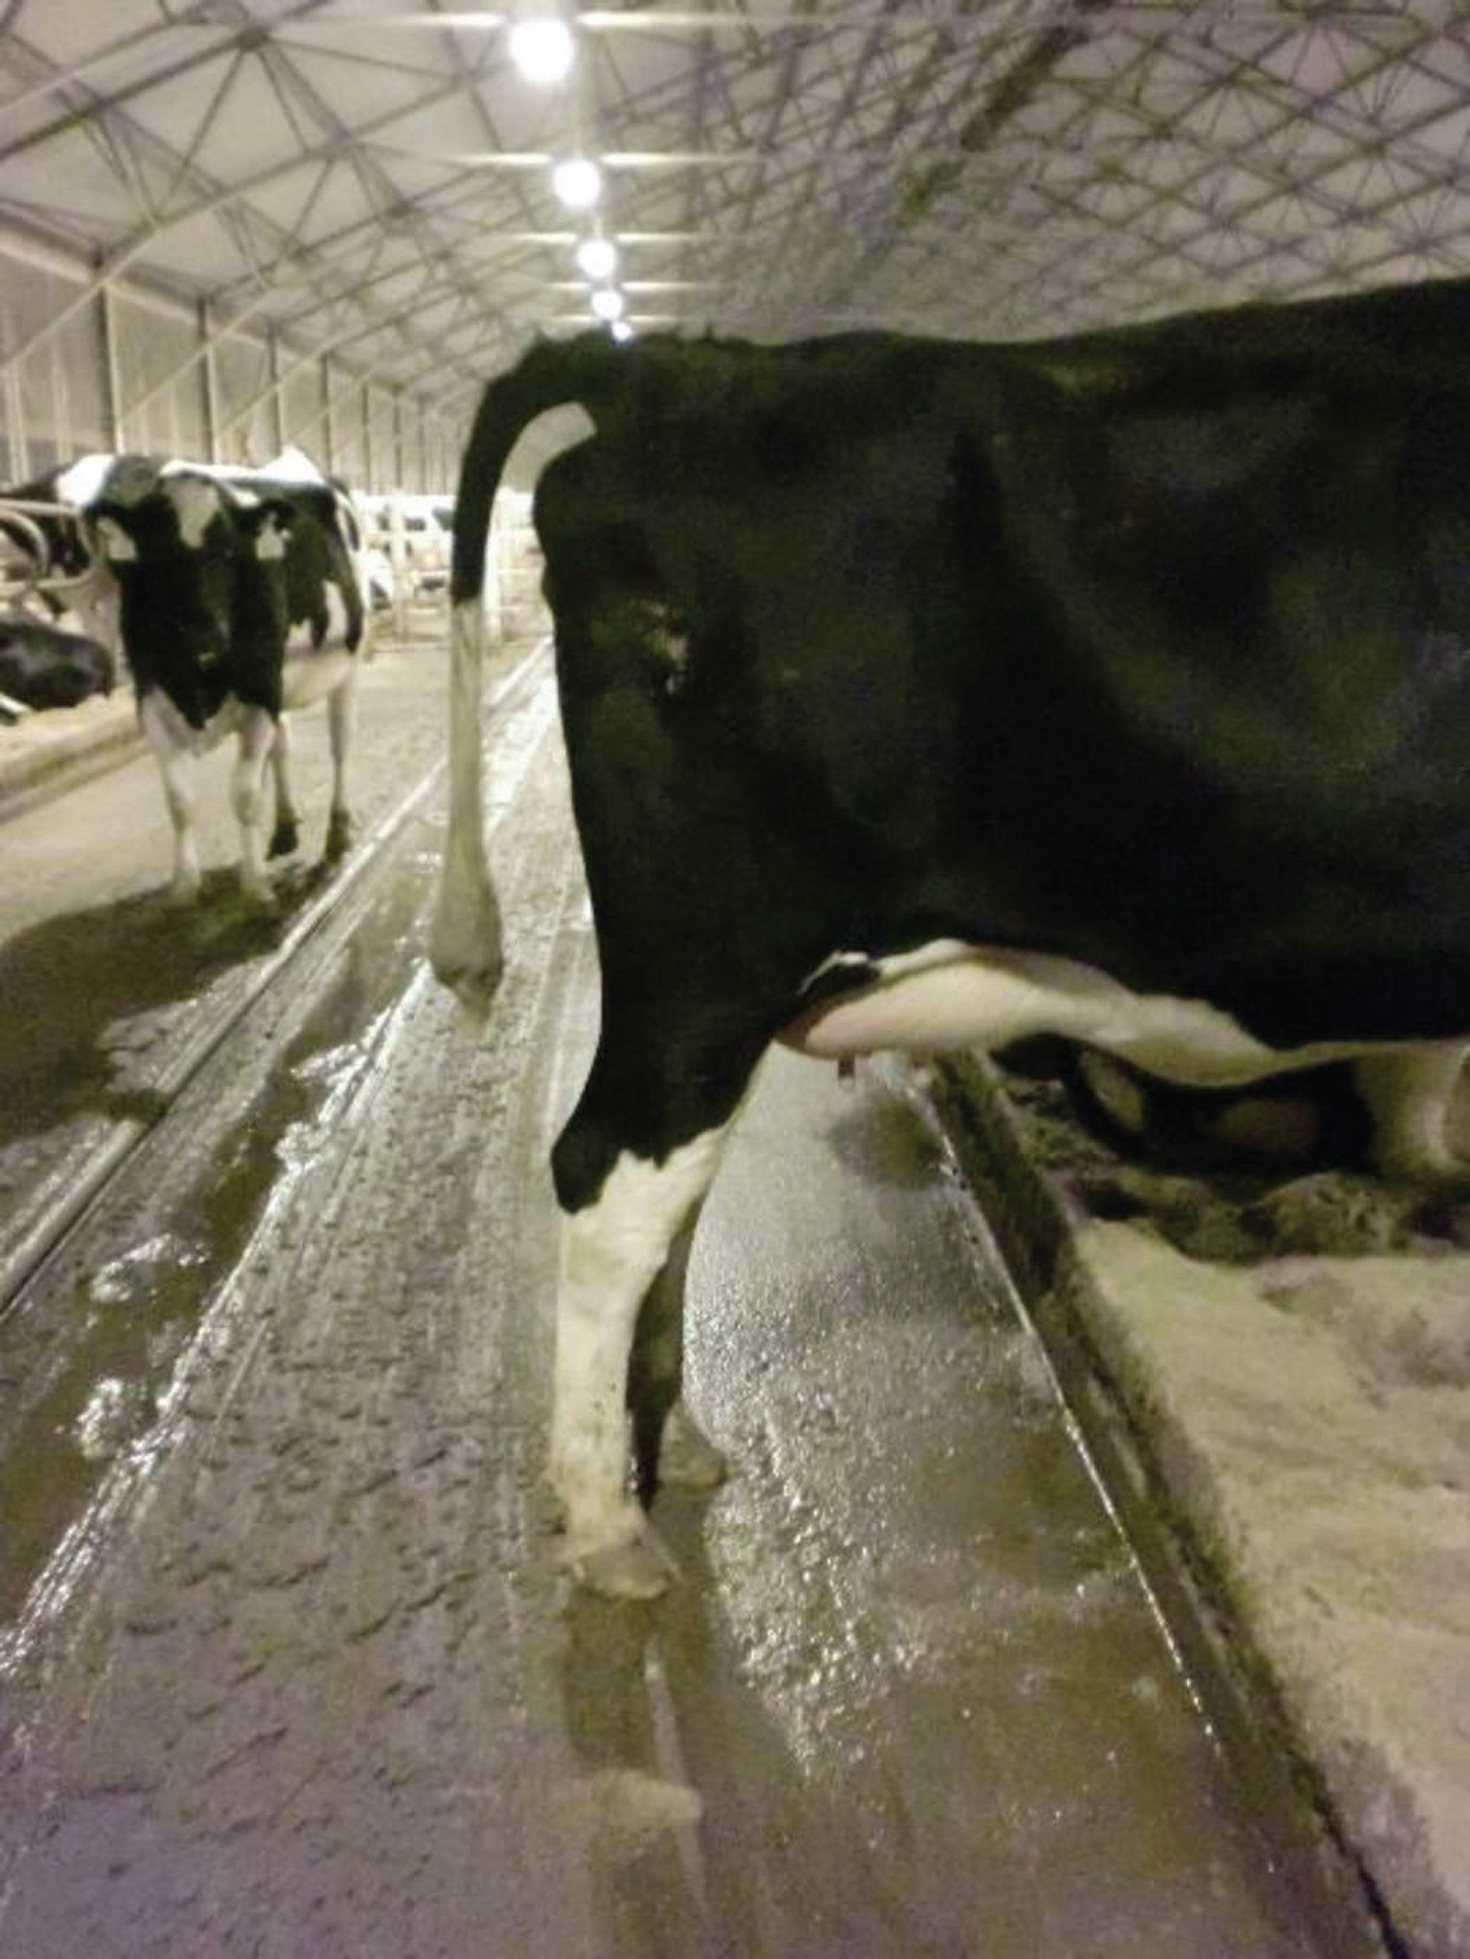
\includegraphics[scale=.45]{Grafiken/schwanzhebung.jpg}
	\caption{Schwanzhebung}
	\label{fig: Schwanzhebung}
\end{figure}

Schwanzhebung wie in Abbildung  \ref{fig: Schwanzhebung} von Lange et al. tritt vermehrt in den letzten $24$ Stunden vor dem Kalben auf \cite[S. 1 f.]{Lange2017}.
\subsection{Zeitliche und prädiktive Hinweise zu den Geburtsanzeichen}
Es ist zu beachten, dass einige Hinweise in erster Linie auf eine Entbindung innerhalb der nächsten vier Tage hinweisen (nachfolgend Vorkalbeperiode genannt), während andere Anzeichen auf eine Geburt innerhalb der nächsten $24$ Stunden hinweisen. Ruhelosigkeit, wiederkehrende Schwanzhebung und die Drehung des Kopfes zum Bauch hin treten häufig $12$ bis $6$ Stunden vor der Geburt auf. Scheidenausfluss weist darauf hin, dass innerhalb der nächsten $6$ Stunden die Geburt eintritt. \citep[S. 1]{Lange2017}

Bereits durchgeführte Experimente von \citep[S. 1]{Lange2017} anhand von stündlicher Beobachtung konnten das Kalben nicht präzise vorhersagen. Demgegenüber konnte das Kalben für die nächsten $12$ Stunden jedoch mit hoher Wahrscheinlichkeit ausgeschlossen werden ($88.5$ bis $97.1$ Prozent). Mit der Information, dass eine Kuh in den nächsten $12$ Stunden nicht kalben wird, können Zeit und Ressourcen bei der Überwachung optimiert werden. Daher sind auch Merkmale zu definieren, welche darauf hinweisen, dass \textit{keine} Geburt stattfindet.

Die wichtigsten Parameter zur Prognose des Kalbens innerhalb der nächsten 12 Stunden sind Beckenbänder, Zitzenfüllung, \gls{Aufeutern}\footnote{\label{glossar-aufeutern}siehe Glossar} und Scheiden- und Euterödeme. Diese Parameter erlauben eine genaue Vorhersage des Ausbleiben des Kalbens \citep[S. 4]{Streyl2011}.



\begin{figure}[H]
	\center
	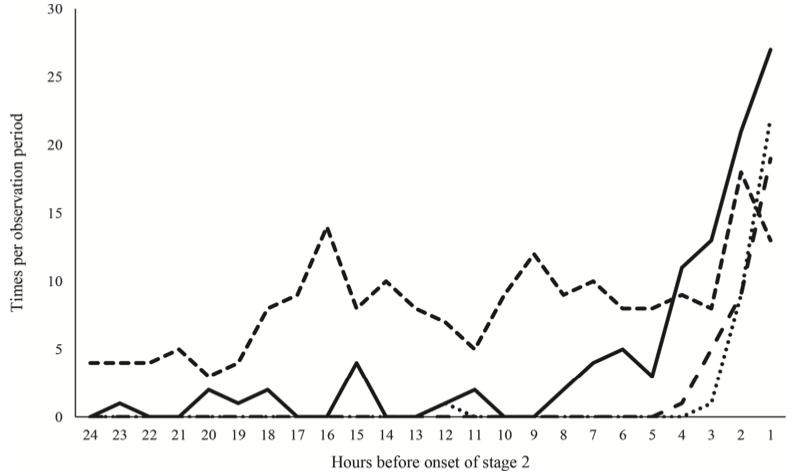
\includegraphics[scale=.45]{Grafiken/observationTimes.png}
	\caption{Häufigkeit von Geburtsanzeichen während den letzten $24$ Stunden vor Geburtsstadium zwei \citep[S.5]{Lange2017}.}
	\label{fig: Häufigkeit von Geburtsanzeichen }
\end{figure}

Die Abbildung \ref{fig: Häufigkeit von Geburtsanzeichen } von Lange et al. zeigt Schwanzhebung als durchgezogene Linie, klarer Scheidenausfluss als kurze gestrichelte Linie,  blutiger Scheidenausfluss als lange gestrichelte Linie und seitliches Liegen mit Abdominalkontraktion als gepunktete Linie
\subsection{Weiterführende Geburtsanzeichen}
Die Geburt eines Kalbs wird durch die \gls{Hypothalamus}\footref{glossar-aufeutern}-\gls{Hypophyse}\footref{glossar-aufeutern}-Nebennieren-rinden-Achse des \gls{Foetus}\footref{glossar-aufeutern} gesteuert. $72$ Stunden vor der Geburt des Kalbs können diverse hormonelle Veränderungen beobachtet werden. Beispielsweise nimmt die \gls{Fetal}\footref{glossar-aufeutern} Produktion von \gls{Kortisol}\footref{glossar-aufeutern} ungefähr $10$ Tage vor der Geburt stark zu, was wiederum das \gls{Progesteron}\footref{glossar-aufeutern}-\gls{Oestradiol}\footref{glossar-aufeutern}-Verhältnis im mütterlichen Blut beeinflusst. Auch Informationen zur Veränderung der Temperatur der äusseren Geschlechtsorgane und zum Wiederkauverhalten können für sensorbasierte Systeme einen deutlichen Mehrwert in Bezug auf die prädiktive Analyse schaffen. Ausserdem versuchen Kühe am Tag der Geburt vermehrt, sich von der Herde zu isolieren \citep[S.1-4]{Saint-Dizier2015}. 
Da die vorliegende Arbeit aber auf die Analyse von Bildern fokussiert, werden diese sozialen Merkmale in der nachfolgenden Arbeit nicht mehr thematisiert. 
\subsection{Ablauf einer normalen Geburt}
Normalerweise befinden sich Kälber in der Vorderendlage. Das heisst, dass zuerst die Vorderbeine und der Kopf durch die Scham gepresst werden \citep{Muller2020}. Eine mögliche Fehlhaltung\footnote{Der zitierte Bericht \glqq Geburtsüberwachung und Geburtshilfe beim Rind\grqq{} veranschaulicht die Fehlhaltungen und mögliche Eingriffe durch Landwirte und Tierärzte.} ist die Hinterendlage. In diesem Fall wird das Kalb mit den Hinterbeinen voran abgekalbert. Weiter stellen Kopfseitenhaltung, Rückenquerlage und gebeugte Gliedmassen ein Risiko für die Geburt dar. Bei der Rückenquerlage ist in der Regel ein Kaiserschnitt notwendig. Die übrigen Fehlhaltungen sind oftmals durch den Landwirten korrigierbar \citep[S. 17, 24-26]{Traulsen2013}.

\begin{figure}[H]
	\center
	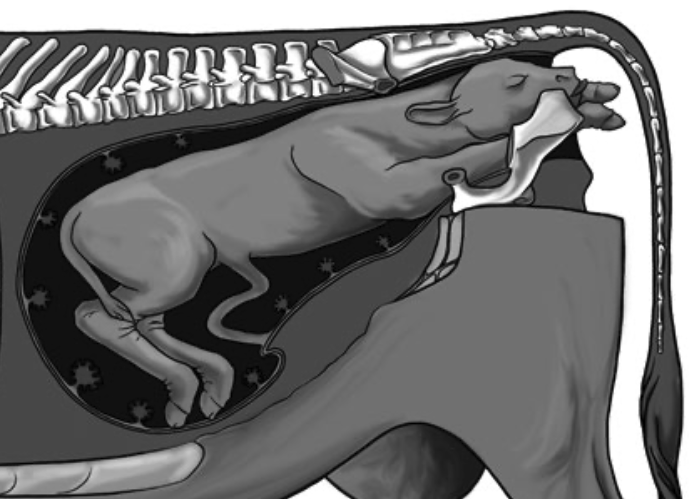
\includegraphics[scale=.45]{Grafiken/vorderendlage.png}
	\caption{Veranschaulichung zur Vorderendlage eines Kalbes \citep[S. 17]{Traulsen2013}.}
	\label{fig: Schwanzhebung}
\end{figure}

Eine Geburt kann in fünf Phasen eingeteilt werde: Vorbereitungsphase, Öffnungsphase, Aufweitungsphase, Austreibungsphase und Nachgeburtsphase \citep[S. 6-8 ]{Traulsen2013}.

In der Vorbereitungsphase stellt sich die Kuh auf die bevorstehende Geburt ein. Deshalb treten die obengenannten Geburtsanzeichen auf. Zwei wichtige Merkmale sind eingefallene Beckenbänder oder rote Färbung der äusseren Geschlechtsorgane \citep[S. 6 ]{Traulsen2013}.  

Die Öffnungsphase erstreckt sich über $6$ bis $16$ Stunden. Der innere Muttermund öffnet sich und die Fruchtblasen treten in den Gebärmutterhals ein, damit dieser gedehnt wird. Es treten erste, leichte Wehen auf und die Kuh kann unruhig sein \citep[S. 7 ]{Traulsen2013}.  

\begin{figure}[H]
	\center
	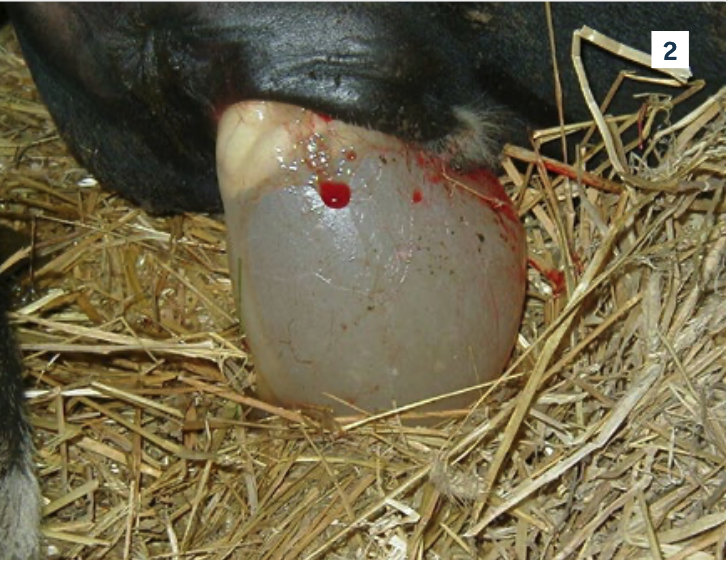
\includegraphics[scale=.45]{Grafiken/oeffnungsphase.png}
	\caption{Wasser- und Schleimblase}
	\label{fig: Öffnungsphase}
\end{figure}

In Abbildung \ref{fig: Öffnungsphase} weiten die Fruchtblasen (Wasser- und Schleimblase) bei der Öffnungsphase den Geburtsweg \citep[S. 7 ]{Traulsen2013}. 

Die Zeit vom Blasensprung bis zum Durchtreten des Kopfes wird als Aufweitungsphase bezeichnet und dauert $1$ bis $6$ Stunden \citep[S. 7 ]{Traulsen2013}. 
\begin{figure}[H]
	\center
	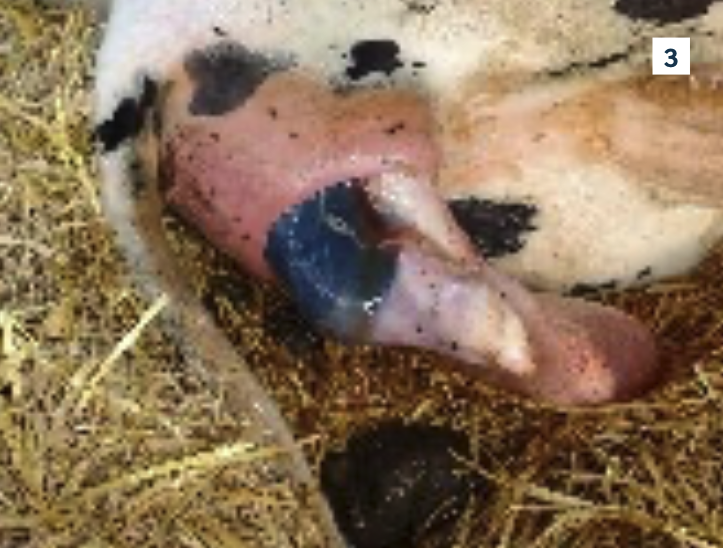
\includegraphics[scale=.45]{Grafiken/aufweitungsphase.png}
	\caption{ Aufweitungsphase }
	\label{fig: Aufweitungsphase}
\end{figure} 

Die Aufweitungsphase ist in Abbildung \ref{fig: Aufweitungsphase} sichtbar und dauert bei Kühen im Normalfall $1$ bis $3$ Stunden. Bei Färsen kann dies bis zu $3$ Stunden länger dauern. \citep[S. 7 ]{Traulsen2013}

Im Rahmen der Austreibungsphase sollte das Kalb in nur $5$ bis $15$ Minuten nach dem Durchtritt des Kopfes durch die Scham geboren sein \citep[S. 8 ]{Traulsen2013}.  


\begin{figure}[H]
	\center
	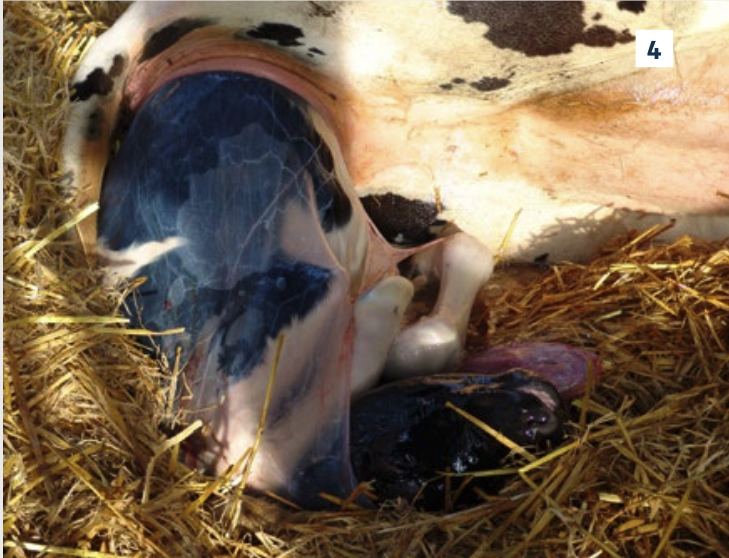
\includegraphics[scale=.45]{Grafiken/austreibungsphase.png}
	\caption{Austreibungsphase}
	\label{fig: Austreibungsphase}
\end{figure}

 In der Austreibungsphase (Abbildung \ref{fig: Austreibungsphase}) wird das Kalb zur Welt gebracht \citep[S. 8 ]{Traulsen2013}

Die Nachgeburtsphase dauert $6$ bis $12$ Stunden und dabei verliert die Kuh das restliche Fruchtwasser und die Nachgeburt \citep[S. 8 ]{Traulsen2013}.  
    
	% ================================================================
% CHAPTER 3: Domänenanalyse: Erkenntnisse aus Interviews
% ================================================================

\section{Erkenntnisse aus den Interviews}

Ziel der Interviews ist einerseits, die Erkenntnisse aus der Literaturrecherche zu validieren und zu ergänzen. Andererseits sollen die Interviews auch Klarheit darüber bringen, wie stark die Anwesenheit oder Abwesenheit von bestimmten Eigenschaften als Hinweis für eine bevorstehende Entbindung gedeutet werden sollen. 

Jedes Merkmal wird bewertet, um zu beschreiben, wie stark dessen Anwesenheit oder Abwesenheit als Indikator einer bevorstehenden Geburt dient.  


\subsection{Kernaussagen aus Interviews}
Gemäss Interview mit Dr. med. vet. Samuel Kohler \citep{Kohler2020} sind viele der Merkmale, die für Geburtsprognosen untersucht werden, eine direkte Folge von erhöhtem Östrogenspiegel. Dies bestätigt, dass die in der Literaturrecherche identifizierten Merkmale wie beispielsweise Scheidenausfluss von einer entsprechenden Software als Geburtsanzeichen gedeutet werden dürfen (ibid.). Die alleinige Anwesenheit eines Merkmals reicht jedoch bis auf wenige Ausnahmen nicht aus, um eine Geburt mit hoher Wahrscheinlichkeit zu prognostizieren. Zudem ist es gemäss Dr. med. vet. Samuel Kohler nicht möglich, aufgrund einer wissenschaftlicher Grundlage Kombinationen von Merkmalen mit entsprechenden Schwellwerten zu nennen, welche mit ausreichender Wahrscheinlichkeit auf eine Geburt hinweisen und dementsprechend eine Benachrichtigung auslösen müssen.

Eine Geburt ist physiologisch betrachtet auch ohne viele der Merkmale wie rötliche Färbung der äusseren Geschlechtsorgane und auch ohne Scheidenausfluss möglich. Demzufolge kann die Abwesenheit der meisten Merkmale nicht verwendet werden, um eine anstehende Geburt in den nächsten Stunden mit Sicherheit auszuschliessen \citep{Kohler2020}. 

Besonders wichtig für die vorliegende Arbeit sind jedoch die prädikativen Merkmale, die immer eine Benachrichtigung auslösen müssen. Einerseits ist dies die Seitenlage mit gestreckten Beinen und andererseits die Anwesenheit der Wasser- oder Schleimblase. Dabei ist die Unterscheidung zwischen Wasserblase und Schleimblase nicht von Bedeutung. Unabhängig davon, welche Blase sichtbar ist, muss das System eine Benachrichtigung auslösen \citep{Kohler2020}.

Die Erkenntnisse aus dem Interview mit Dr. med. vet. Gaby Hirsbrunner \citep{Hirsbrunner2020} stützen die Kernaussagen aus dem Interview mit Dr. med. vet. Samuel Kohler und das gewonnene Wissen aus der Literaturrecherche. Seitenlage und Sichtbarkeit der Wasser- oder Schleimblase gehören erneut zu den wichtigsten Geburtsanzeichen, die auf Bildern erfasst werden können. Dies bestätigt die Meinung, dass jedes dieser Merkmale auch ohne die Anwesenheit von weiteren Geburtsanzeichen eine Benachrichtigung an den Landwirten auslösen soll. Zudem bestätigt Dr. med. vet. Gaby Hirsbrunner	die Meinung, dass die Abwesenheit der meisten Merkmale nicht in die Geburtsprognose einfliessen sollte.  

Die Aussagen von Dr. med. vet. Gaby Hirsbrunner verfeinern das Domänenwissen, indem die Merkmale Seitenlage für Anbdindehaltung und Freilauf getrennt bewertet werden. Gemäss \citep{Hirsbrunner2020} ist bei Anbindehaltung seitliches Liegen fast nur bei einer anstehenden Geburt zu beobachten ($Bewertung=9$). Bei der Haltung in Freilauf kann dies durchaus häufiger geschehen und ist dementsprechend auch ein schwächerer Indikator für eine anstehende Geburt ($Bewertung=4$).

Zudem sind weitere Erkenntnisse zur Erkennung von erschwerter Geburt für die vorliegende Arbeit besonders wertvoll. Blutiger Scheidenausfluss soll unbedingt als alarmierendes Zeichen interpretiert werden. Auch häufiges Trippeln kann als Symptom einer Verdrehung der Gebärmutter (Überwurf) auftreten. Sowohl blutiger Scheidenausfluss als auch häufiges Trippeln müssen daher eine Benachrichtigung auslösen \citep{Hirsbrunner2020}.

Das beschriebene System muss für einen zweckmässigen Einsatz in der Landwirtschaft und im Veterinärwesen zuverlässig, kostengünstig und einfach in der Handhabung sein \citep{Hirsbrunner2020}. Um möglichst viele visuelle Hinweise zu den Merkmalen zu erfassen, ist die Kamera hinter der Kuh zu platzieren \citep{Hirsbrunner2020, Kohler2020}. Zudem soll die Kamera einen möglichst breiten Blickwinkel abdecken, damit die Kuh nicht aus dem Sichtfeld verschwindet \cite{Muller2020}. Da laut der Meinung der Experten die Festlegung von Schwellwerten und Dimensionen während der Aufnahme nicht möglich ist \citep{Hirsbrunner2020, Kohler2020}, besteht der Benachrichtigungstext aus dem Namen des auftretenden Merkmals und einer zeitlichen Angabe.

\subsection{Codierung von Domänenwissen aus Interviews}

In Tabelle \ref{tab: Bewertung der Anwesenheit und Abwesenheit von Merkmalen} wird Domänenwissen von Prof. Dr. med. vet. Samuel Kohler und  Dr. med. vet. Gaby Hirsbrunner codiert. Dieses wurde bei Interviews per Videotelefonie erhoben. Beide befragte Personen haben die An- und Abwesenheit von Merkmalen in Bezug auf die Stärke des Hinweises auf eine bevorstehende Geburt bewertet

Die Tabelle \ref{tab: Bewertung der Anwesenheit und Abwesenheit von Merkmalen} besteht nebst der Aufzählung von Merkmalen aus den drei Spaltengruppen \flqq{}Anwesenheit\frqq{}, \flqq{}Abwesenheit\frqq{} und \flqq{}Mittelwert\frqq{} (horizontale Beschriftung). Die Gruppen \flqq{}Anwesenheit\frqq{} und \flqq{}Abwesenheit\frqq{} repräsentieren dabei die Rohdaten, welche auf der Durchführung von Interviews basieren. Die Spalten der Gruppe \flqq{}Mittelwert\frqq{} entsprechen jeweils dem gewichteten Mittelwert der Rohdaten aus den vorgelagerten Spaltengruppen.

Für die gesammelten Daten zur An- und Abwesenheit von Merkmalen sind je vier Spalten vorhanden. Eine Spalte repräsentiert jeweils die Bewertungen der Tierärzte und eine weitere Spalte entspricht der Gewichtung dieser Bewertung. In Klammer sind die Initialen des Interviewten angegeben, also \texttt{SK} für Prof. Dr. med. vet. Samuel Kohler und  \texttt{GH} für Dr. med. vet. Gaby Hirsbrunner.

Während der Durchführung der Interviews hatten die ExpertInnen die Möglichkeit, weitere Geburtsmerkmale hinzuzufügen und zu bewerten. Deshalb haben nicht beide Veterinäre sämtliche Merkmale bewertet. Falls einer davon die Anwesenheit oder Abwesenheit eines Merkmals nicht bewertet hat, ist dies mit $Bewertung=99$ codiert. Diese Bewertung wird dementsprechend nicht gewichtet, also \newline $Gewichtung=0$. 

Der gewichtete Mittelwert der Bewertung von An- und Abwesenheit dieser Merkmale dient als integraler Bestandteil des zu entwickelnden Systems. Dieses muss das gewonnene Domänenwissen einsetzen, um Kamerabilder mit Abkalbung von Kamerabildern ohne Abkalbung zu unterscheiden.




	% ================================================================
% CHAPTER 3: Domänenanalyse: Erkenntnisse aus Interviews: Tabelle mit Codierung 1
% ================================================================


\newgeometry{margin=2.5cm} % Ränder kleiner	
\begin{landscape}

\begin{table}[h]
	\rowcolors{2}{maroon!10}{white!100}
	\arrayrulecolor{darkmaroon} 
	
	\setlength{\tabcolsep}{12pt} % Zellen breiter machen
	

	
	%\begin{tabular}{  p{8.5cm}  c c c c c c c c c c  }
	\begin{tabular}{  p{8.5cm}  l*{10}{l}}
 	  			
	\toprule[1pt]

 	\rowcolor{maroon!30}
	\multicolumn{1}{c}{ }&
	\multicolumn{4}{c}{ Anwesenheit }&
	\multicolumn{4}{c}{Abwesenheit }&
	\multicolumn{2}{c}{Mittelwert }\\

	\cmidrule(lr{3pt}){2-5}
	\cmidrule(lr{3pt}){6-9}
	\cmidrule(lr{3pt}){10-11}
	
	\rowcolor{maroon!30}  
	{\large \textbf{Merkmal}}&
	\rotatebox{90}{\large \textbf{{Bewertung \texttt{SK}}}}  & 
	\rotatebox{90}{\large \textbf{{Gewichtung \texttt{SK}}}} &
	\rotatebox{90}{\large \textbf{{Bewertung \texttt{GH}}}} & 
	\rotatebox{90}{\large \textbf{{Gewichtung \texttt{GH}}}} & 
	\rotatebox{90}{\large \textbf{{Bewertung \texttt{SK}}}} &
	\rotatebox{90}{\large \textbf{{Gewichtung \texttt{SK}}}}  &
	\rotatebox{90}{\large \textbf{{Bewertung \texttt{GH}}}}  &
	\rotatebox{90}{\large \textbf{{Gewichtung \texttt{GH} }}}  &
	\rotatebox{90}{\large \textbf{{Anwesenheit}}}  &
	\rotatebox{90}{\large \textbf{{Abwesenheit}}}  \\
	
	%\midrule[1pt]
	\cmidrule(lr{3pt}){2-5}
	\cmidrule(lr{3pt}){6-9}
	\cmidrule(lr{3pt}){10-11}		
			
Wiederkehrende Schwanzhebung & 3 & 1 & 6 & 1 & -2 & 1 & 0 & 1 & 4.5 & -1.0 \\ 
Wiederholtes Aufstehen und Abliegen & 9 & 1 & 6 & 1 & -2 & 1 & 0 & 1 & 7.5 & -1.0 \\ 
Häufiges hin-und-her-Treten (Trippeln) & 7 & 1 & 2 & 1 & -2 & 1 & 0 & 1 & 4.5 & -1.0 \\ 
Drehung des Kopfes zum Bauch hin & 8 & 1 & 8 & 1 & -7 & 1 & 0 & 1 & 8.0 & -3.5 \\ 
Rote Färbung der äusseren Geschlechtsorgane & 4 & 1 & 0 & 1 & -2 & 1 & 0 & 1 & 2.0 & -1.0 \\ 
Blutiger Scheidenausfluss & 3 & 1 & 1 & 1 & -2 & 1 & 0 & 1 & 2.0 & -1.0 \\ 
Klarer Scheidenausfluss & 3 & 1 & 1 & 1 & -2 & 1 & 0 & 1 & 2.0 & -1.0 \\ 
Eingefallene Beckenbänder & 9 & 1 & 10 & 1 & -8 & 1 & -7 & 1 & 9.5 & -7.5 \\ 
Euterödem & 2 & 1 & 7 & 1 & -1 & 1 & -9 & 1 & 4.5 & -5.0 \\ 
Glänzende Zitzen & 4 & 1 & 8 & 1 & -2 & 1 & -9 & 1 & 6.0 & -5.5 \\ 
Tropfende Milch & 6 & 1 & 2 & 1 & -2 & 1 & 0 & 1 & 4.0 & -1.0 \\ 
Hyperplasie des Euters & 1 & 1 & 6 & 1 & -1 & 1 & 0 & 1 & 3.5 & -0.5 \\ 
Schleimsekretion & 8 & 1 & 6 & 1 & -2 & 1 & 0 & 1 & 7.0 & -1.0 \\ 
Schamlippenödem & 6 & 1 & 7 & 1 & -8 & 1 & 0 & 1 & 6.5 & -4.0 \\ 
Seitliches Liegen & 8 & 1 & 99 & 0 & 99 & 0 & 0 & 1 & 8.0 & 0.0 \\ 
Seitliches Liegen bei Anbindehaltung (nur \texttt{GH}) & 99 & 0 & 9 & 1 & 99 & 0 & 99 & 0 & 9.0 & 0.0 \\ 
Seitliches Liegen bei Freilauf (nur \texttt{GH}) & 99 & 0 & 4 & 1 & 99 & 0 & 99 & 0 & 4.0 & 0.0 \\ 
Seitliches Liegen mit Abdominalkontraktion & 10 & 1 & 10 & 1 & -7 & 1 & 0 & 1 & 10.0 & -3.5 \\ 
Wasser- und Schleimblase & 99 & 0 & 10 & 1 & 99 & 0 & 0 & 1 & 10.0 & 0.0 \\ 
		\bottomrule

	\end{tabular}
	\caption{Bewertung der Anwesenheit und Abwesenheit von Merkmalen als Indikator einer bevorstehenden Geburt. }
	\label{tab: Bewertung der Anwesenheit und Abwesenheit von Merkmalen}
\end{table}

\end{landscape}
\restoregeometry % Wieder die alten Ränder




	% ================================================================
% CHAPTER 3: Domänenanalyse: Erkenntnisse aus Interviews: Tabelle mit Codierung 1
% ================================================================


\newgeometry{margin=2.5cm} % Ränder kleiner	
\begin{landscape}

\begin{table}[h]
	\rowcolors{2}{maroon!10}{white!100}
	\arrayrulecolor{darkmaroon} 
	
	\setlength{\tabcolsep}{18pt} % Zellen breiter machen
	
	\begin{tabular}{  p{8.5cm}  l*{7}{l}}
 	  			
	\toprule[1pt]

	\rowcolor{maroon!30}  
	{\large \textbf{Merkmal}}&
	\rotatebox{90}{\large \textbf{{Häufigkeit }}}  & 
	\rotatebox{90}{\large \textbf{{Vorbereitungsphase (4 Tage) }}} &
	\rotatebox{90}{\large \textbf{{Vorbereitungsphase (24h) }}} & 
	\rotatebox{90}{\large \textbf{{Öffnungsphase }}} & 
	\rotatebox{90}{\large \textbf{{Aufweitungsphase}}} &
	\rotatebox{90}{\large \textbf{{Austreibungsphase }}}  &
	\rotatebox{90}{\large \textbf{{Nachgeburtsphase }}} \\
	
	\midrule[1pt]
		
Wiederkehrende Schwanzhebung & häufig & x & x &  &  &  &  \\ 
Wiederholtes Aufstehen und Abliegen & häufig &  & x &  &  &  &  \\ 
Häufiges hin-und-her-Treten (Trippeln) & häufig &  & x &  &  &  &  \\ 
Drehung des Kopfes zum Bauch hin & immer & x & x &  &  &  &  \\ 
Rote Färbung der äusseren Geschlechtsorgane & häufig &  & x & x &  &  &  \\ 
Blutiger Scheidenausfluss & häufig &  & x & x &  &  &  \\ 
Klarer Scheidenausfluss & häufig &  & x & x &  &  &  \\ 
Eingefallene Beckenbänder & immer & x & x &  &  &  &  \\ 
Euterödem & häufig & x & x &  &  &  &  \\ 
Glänzende Zitzen & häufig & x & x &  &  &  &  \\ 
Tropfende Milch & selten-häufig & x & x &  &  &  &  \\ 
Hyperplasie des Euters & immer & x &  &  &  &  &  \\ 
Schleimsekretion & häufig &  & x & x &  &  &  \\ 
Schamlippenödem & immer & x & x &  &  &  &  \\ 
Seitliches Liegen mit Abdominalkontraktion & immer &  &  & x & x & x &  \\ 
		\bottomrule

	\end{tabular}
	\caption{Zuordnung von Merkmalen zu Geburtsphasen und Bewertung der Häufigkeiten von Merkmalen (Samuel Kohler) }
	\label{tab: Zuordnung und Bewertung der Häufigkeiten von Merkmalen (Samuel Kohler)}
\end{table}

% Datentabelle von Gaby Hirsbrunner weiter unten




















\begin{table}[h]
	\rowcolors{2}{maroon!10}{white!100}
	\arrayrulecolor{darkmaroon} 
	
	\setlength{\tabcolsep}{20pt} % Zellen breiter machen
	

	\begin{tabular}{  p{8.5cm}  l*{6}{l}}
		
		\toprule[1pt]
		
		
		\rowcolor{maroon!30}  
		{\large \textbf{Merkmal}}&
		\rotatebox{90}{\large \textbf{{Häufigkeit }}}  & 
		\rotatebox{90}{\large \textbf{{Vorbereitungsphase (4 Tage) }}} &
		\rotatebox{90}{\large \textbf{{Vorbereitungsphase (24h) }}} & 
		\rotatebox{90}{\large \textbf{{Eröffnungsphase  }}} & 
		\rotatebox{90}{\large \textbf{{Austreibungsphase }}}  &
		\rotatebox{90}{\large \textbf{{Nachgeburtsphase }}}  \\

		
		\midrule[1pt]
		
Wiederkehrende Schwanzhebung & häufig &  & x & x &  &  \\ 
Wiederholtes Aufstehen und Abliegen & häufig &  &  & x &  &  \\ 
Häufiges hin-und-her-Treten (Trippeln) & selten & x & x &  &  &  \\ 
Drehung des Kopfes zum Bauch hin & häufig &  &  &  & x &  \\ 
Rote Färbung der äusseren Geschlechtsorgane & nicht zutreffend &  &  &  &  &  \\ 
Blutiger Scheidenausfluss & nicht zutreffend &  &  &  &  &  \\ 
Klarer Scheidenausfluss & immer & x &  &  &  &  \\ 
Eingefallene Beckenbänder & immer & x & x &  &  &  \\ 
Euterödem & selten & x & x &  &  &  \\ 
Glänzende Zitzen & häufig &  & x & x &  &  \\ 
Tropfende Milch & häufig &  & x & x &  &  \\ 
Hyperplasie des Euters & immer & x & x &  &  &  \\ 
Schleimsekretion & immer & x &  &  &  &  \\ 
Schamlippenödem & häufig & x & x &  &  &  \\ 
Seitliches Liegen ohne Abdominalkontraktion & häufig &  &  &  & x &  \\ 
Seitliches Liegen mit Abdominalkontraktion & immer &  &  &  & x &  \\ 
Wasserblase & immer &  &  & x &  &  \\ 
Schleimblase & immer &  &  &  & x &  \\
		\bottomrule
		
	\end{tabular}
	\caption{Zuordnung von Merkmalen zu Geburtsphasen und Bewertung der Häufigkeiten von Merkmalen (Gaby Hirsbrunner) }
	\label{tab: Zuordnung und Bewertung der Häufigkeiten von Merkmalen (Gaby Hirsbrunner)}
\end{table}




\end{landscape}
\restoregeometry % Wieder die alten Ränder



	
	% ================================================================
% CHAPTER 3: Domänenanalyse: Domänenmodell
% ================================================================

\section{Bildmaterial aus ersten Tests}

In der Nacht vom 31. März 2020 auf den 1. April 2020 ist auf dem Betrieb vom Auftraggeber Peter Müller ein Kalb geboren. Das Bildmaterial zur Geburt zeigt einige Geburtsanzeichen, welche Merkmale aus der Literaturrecherche und aus Interviews beispielhaft veranschaulichen. Zudem ist auf den Bildern gemäss Aussage von \citep{Muller2020a} deutlich erkennbar, wie die Klauen des Kalbes aus der Kuh austreten. Diese Erkenntnis ergänzt das Wissen aus der der bisherigen Domänenanalyse. Folgend die wichtigsten Ergebnisse von der Klassifikation der Kamerabilder. \\





\begin{figure}[h]
	\center
	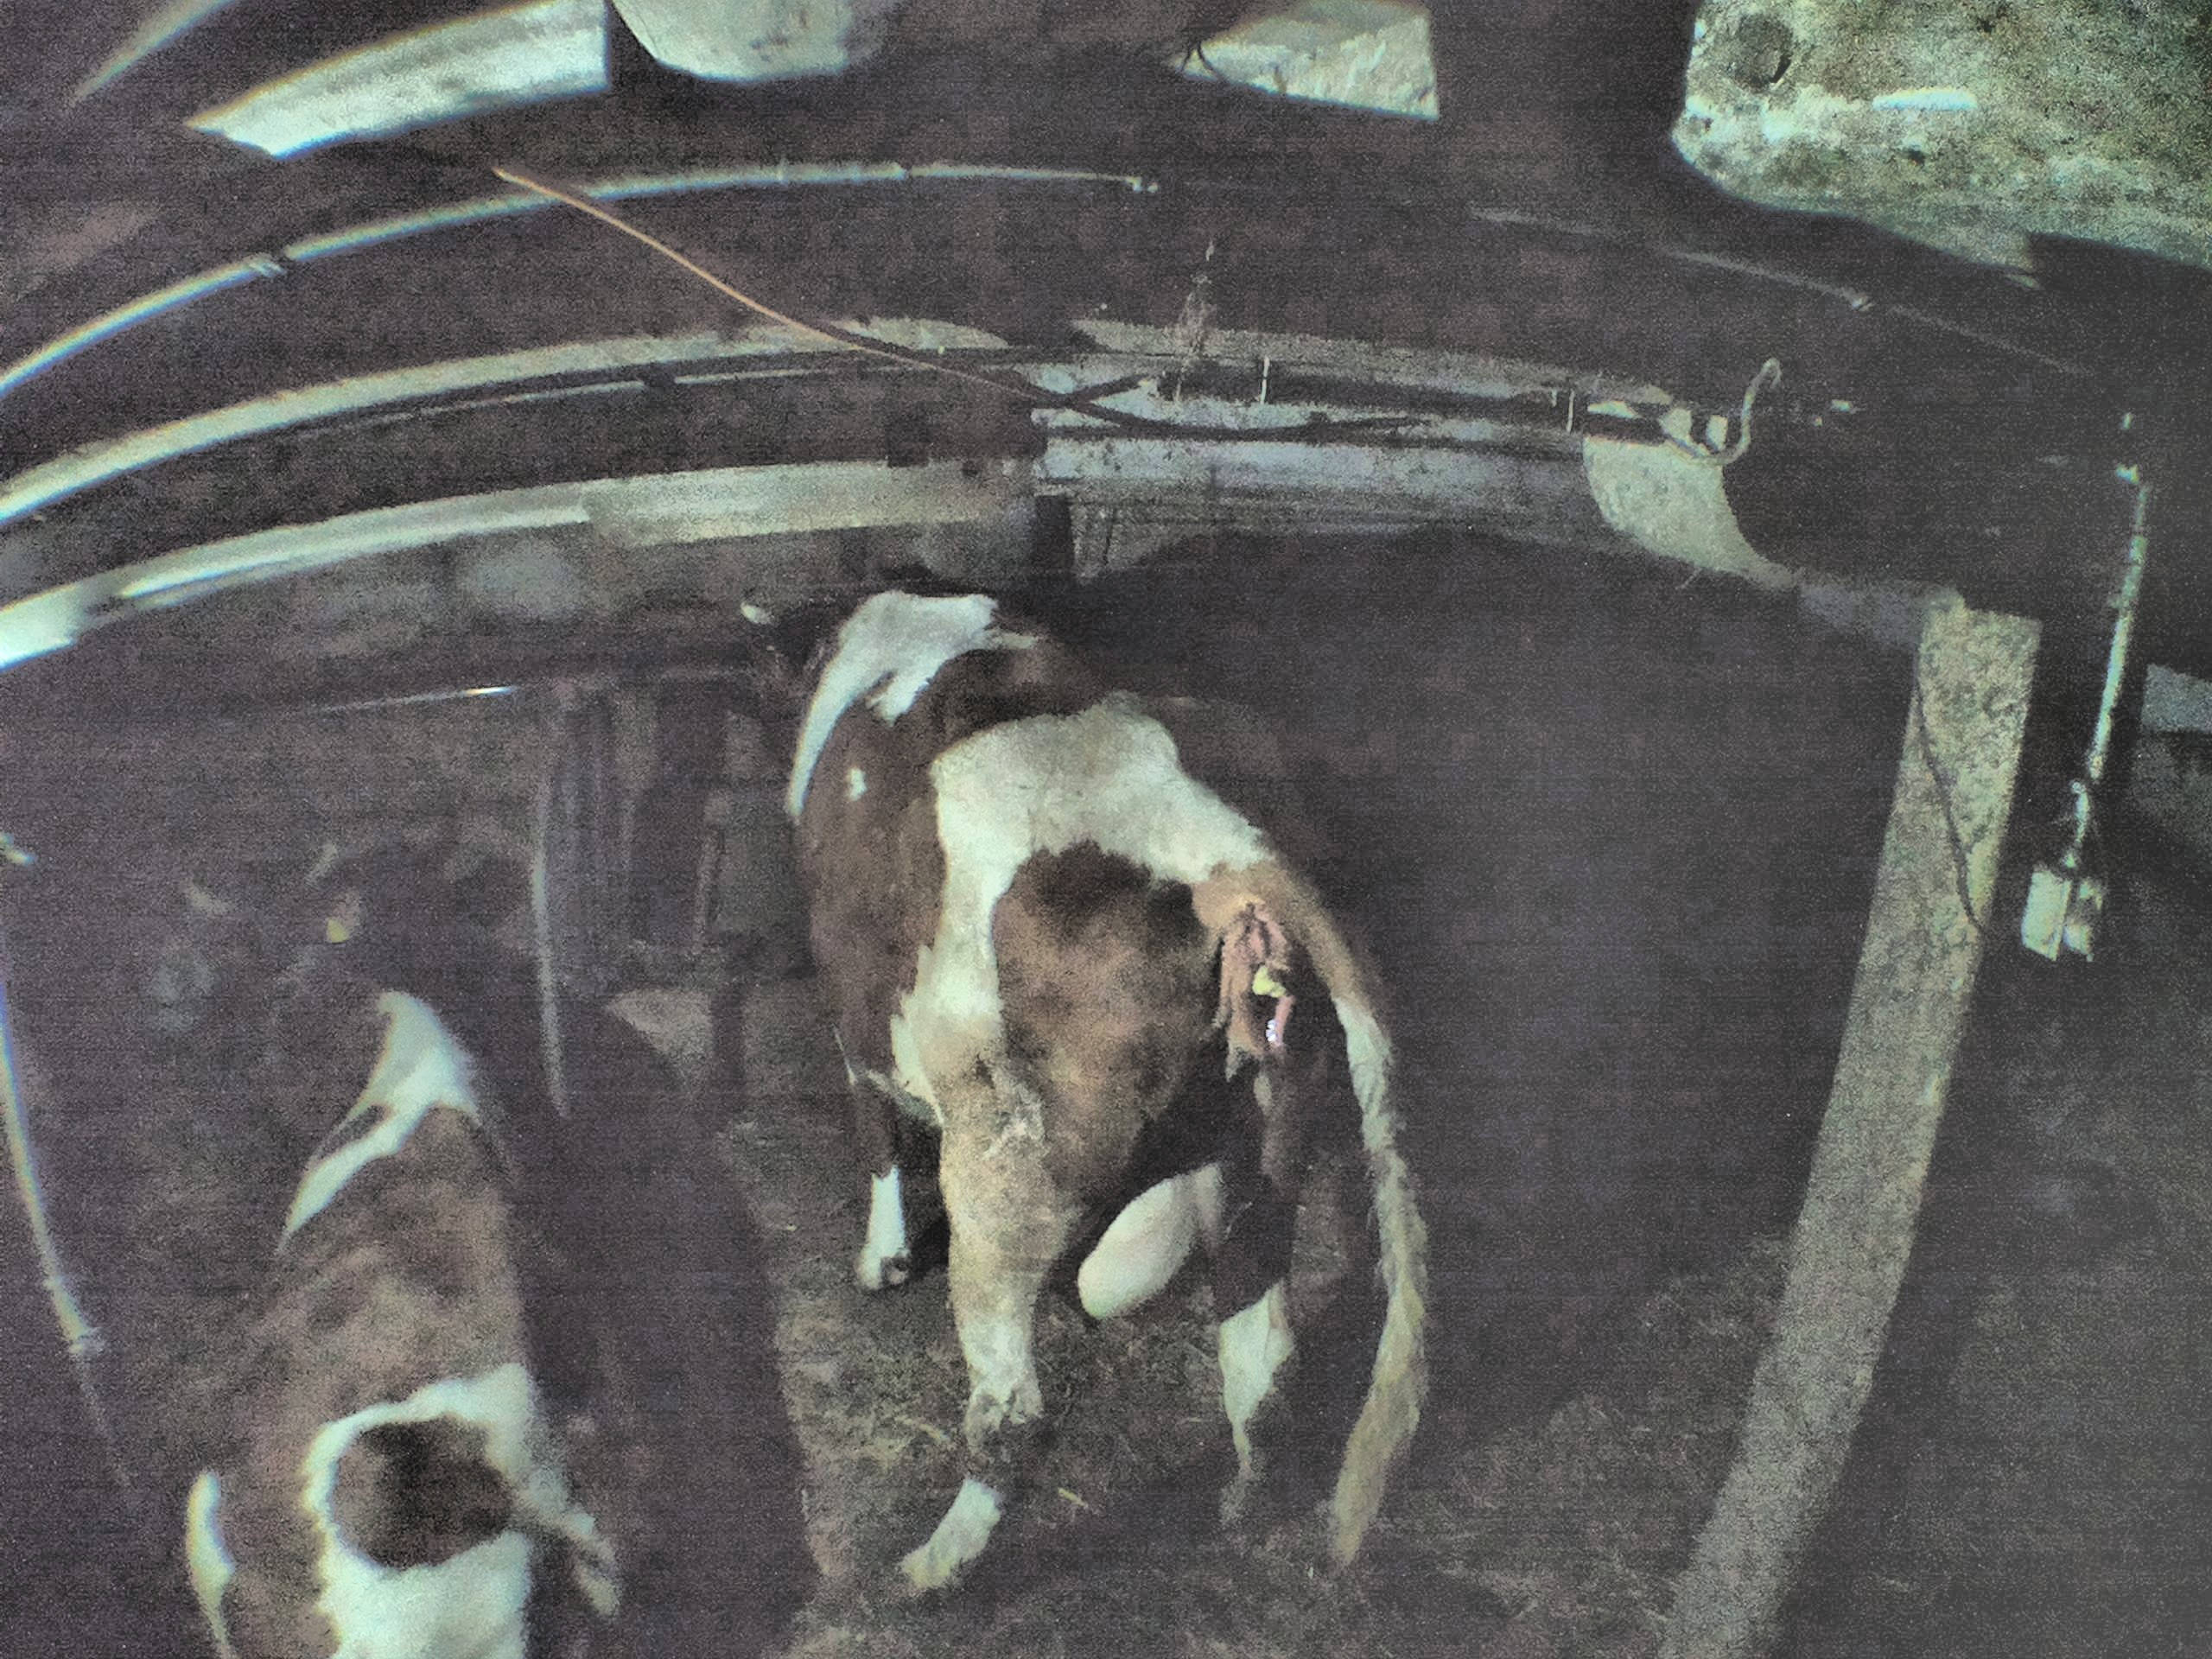
\includegraphics[scale=0.075]{Grafiken/austrittklauen.jpg}
	\caption{Austritt der Klauen des Kalbes \citep{Muller2020a}} 
	\label{fig: Austritt der Klauen des Kalbes}
\end{figure}


\begin{figure}[h]
	\center
	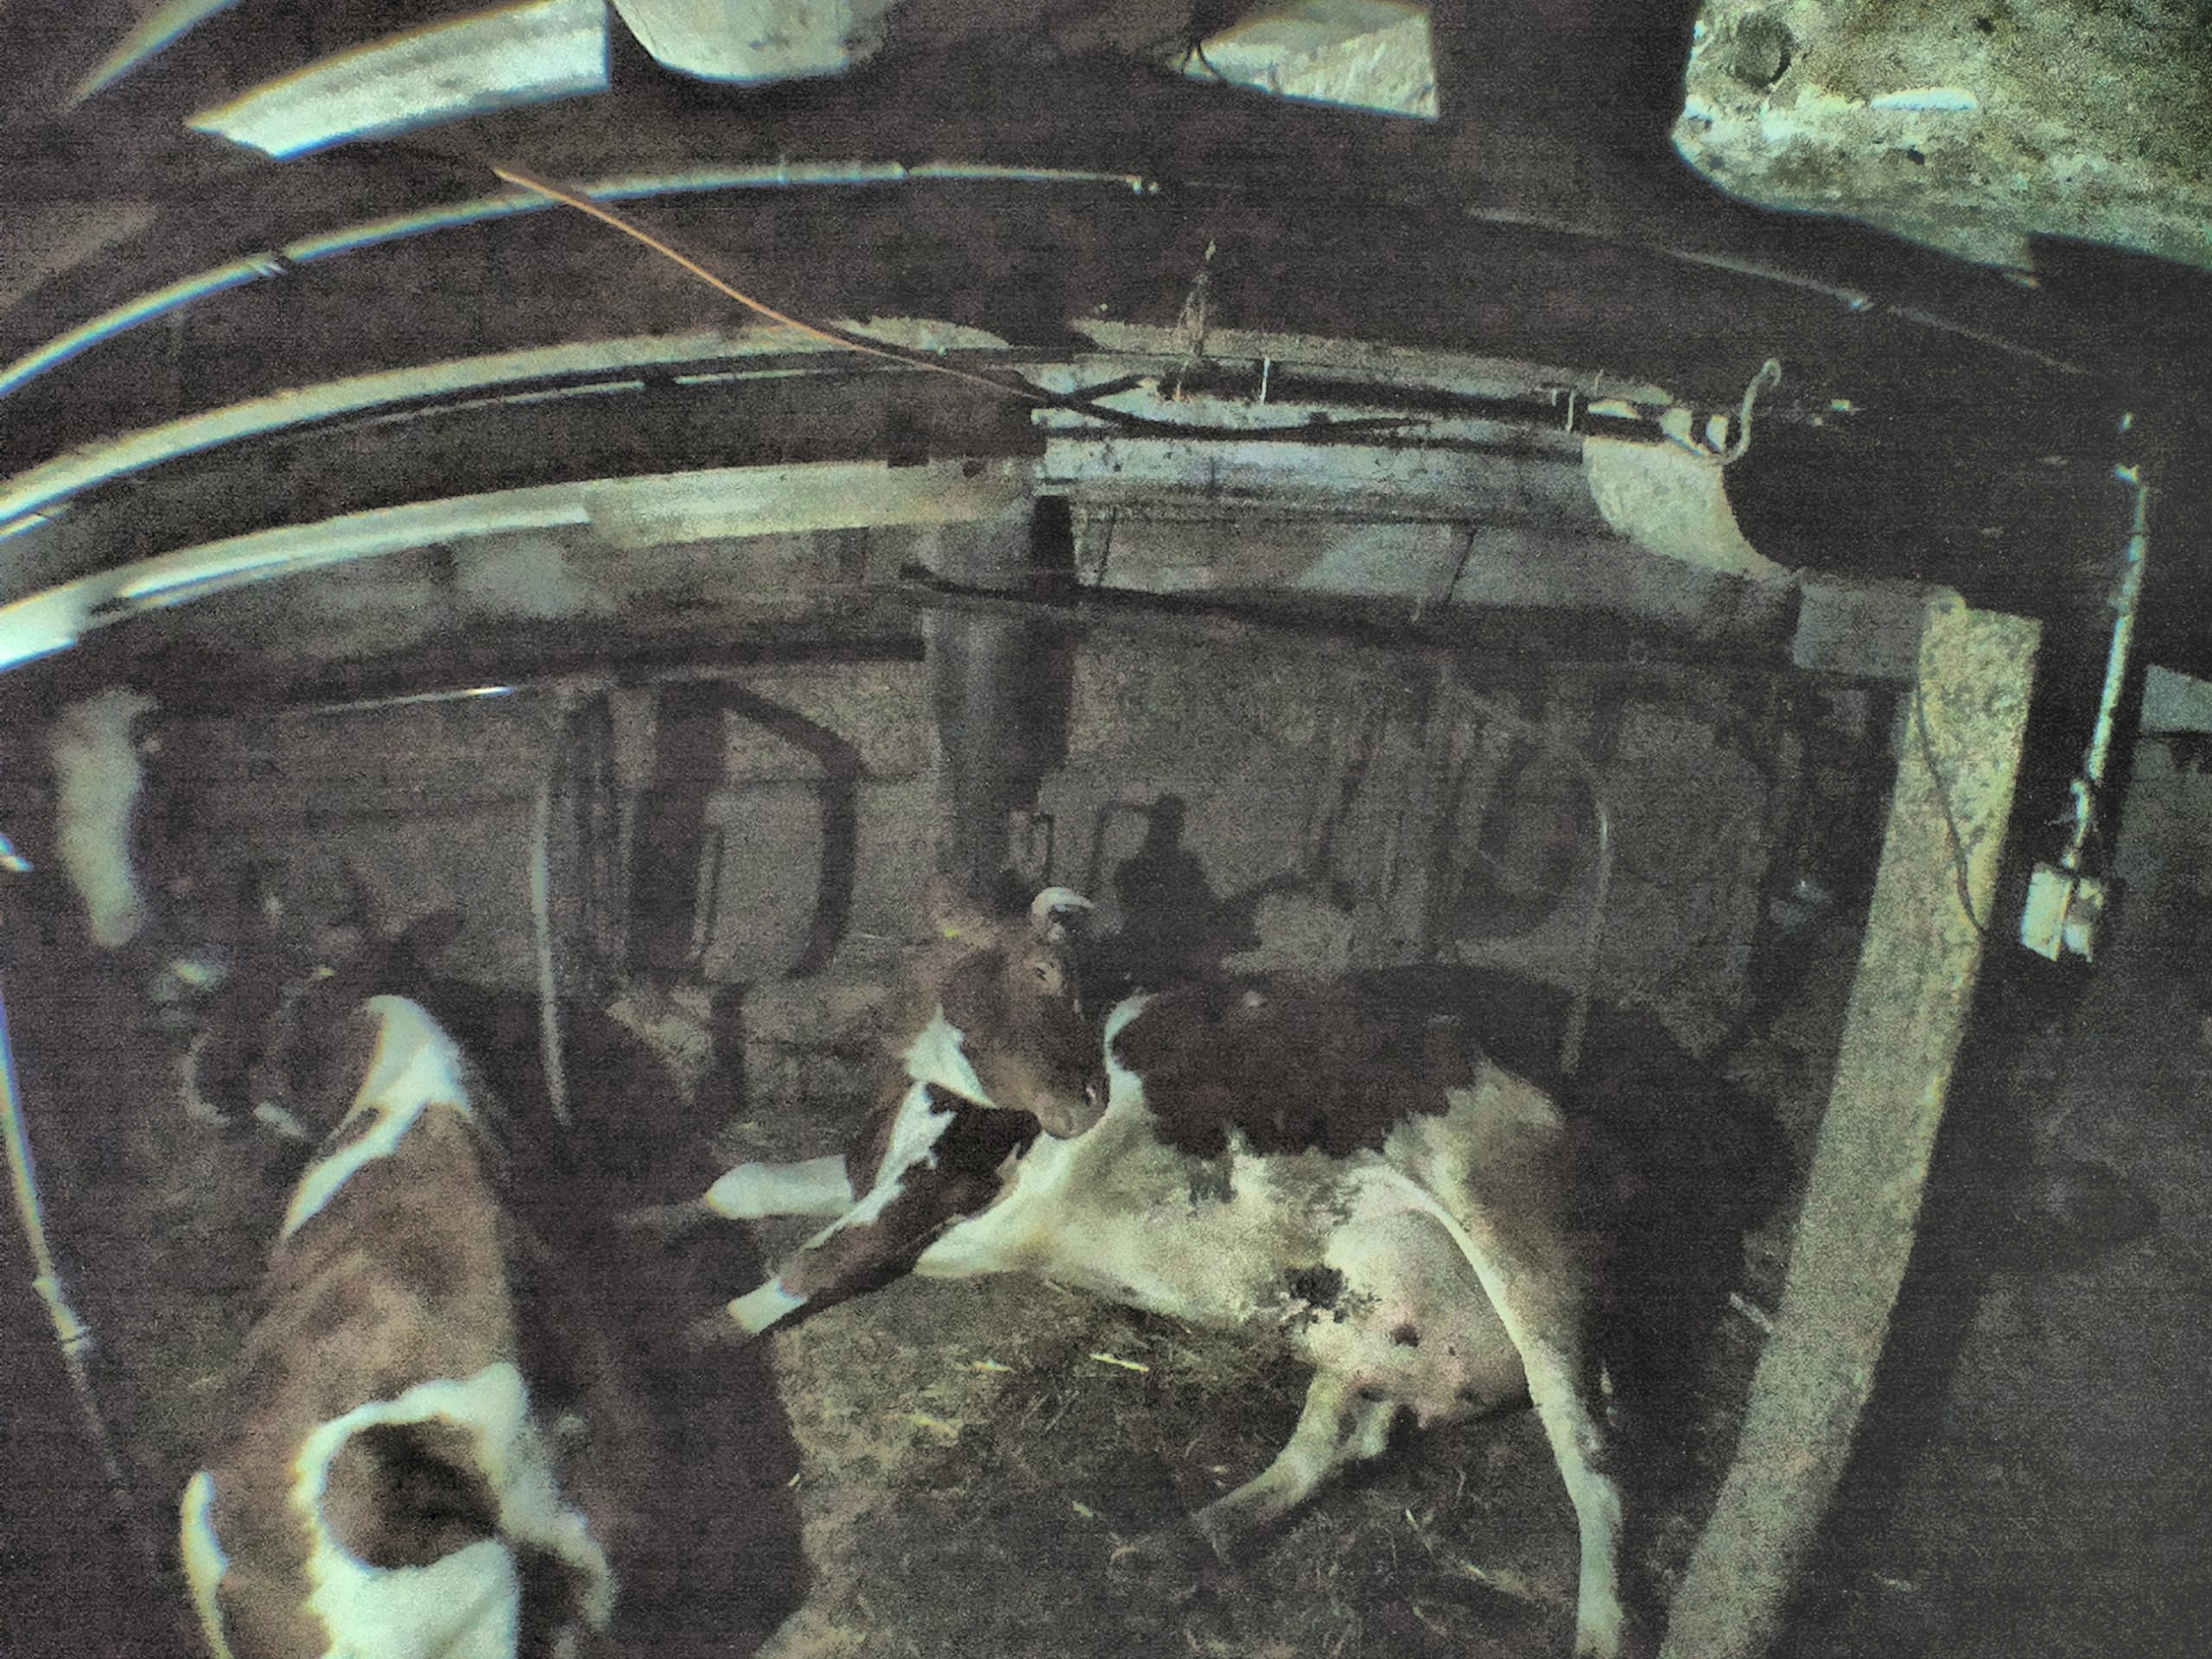
\includegraphics[scale=0.075]{Grafiken/seitlichesligen.jpg}
	\caption{Seitliches Liegen kurz vor der Geburt des Kalbes} 
	\label{fig: Seitliches Liegen kurz vor der Geburt des Kalbes}
\end{figure}


\begin{figure}[h]
	\center
	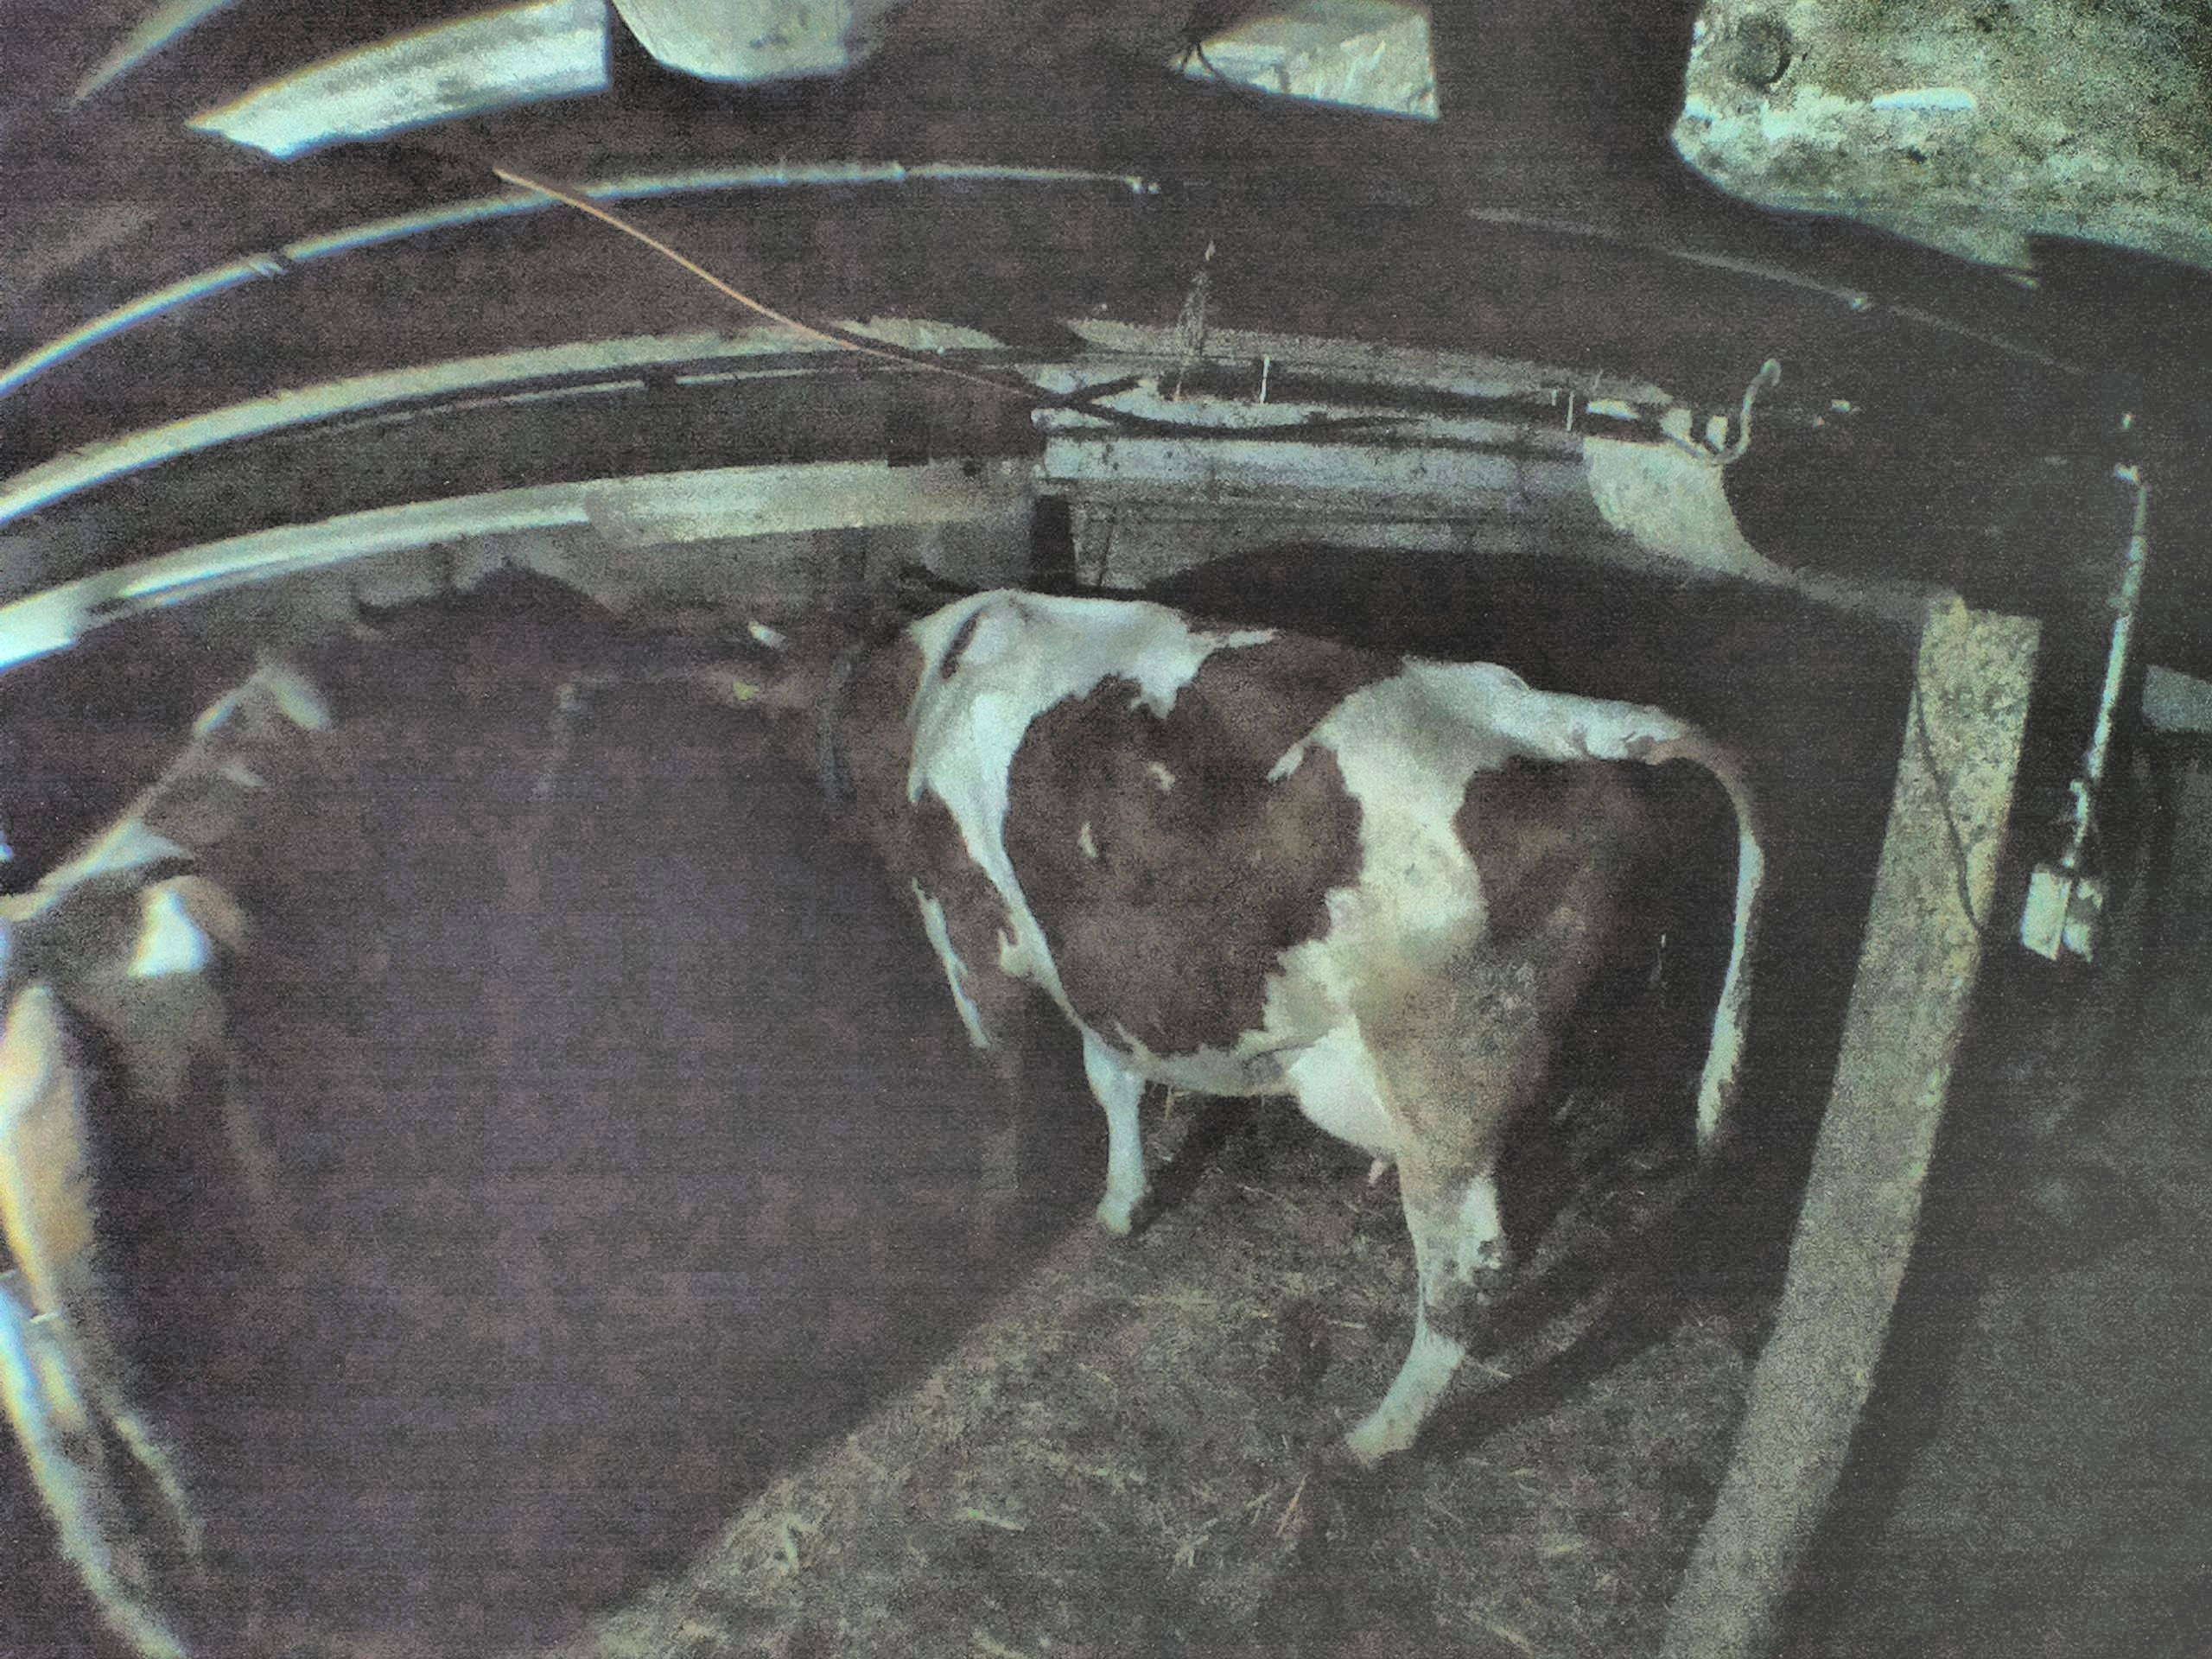
\includegraphics[scale=0.075]{Grafiken/schwanhebungkamerabild.jpg}
	\caption{Kamerabild bei Schwanzhebung} 
	\label{fig: Kamerabild bei Schwanzhebung}
\end{figure}

\begin{figure}[h]
	\center
	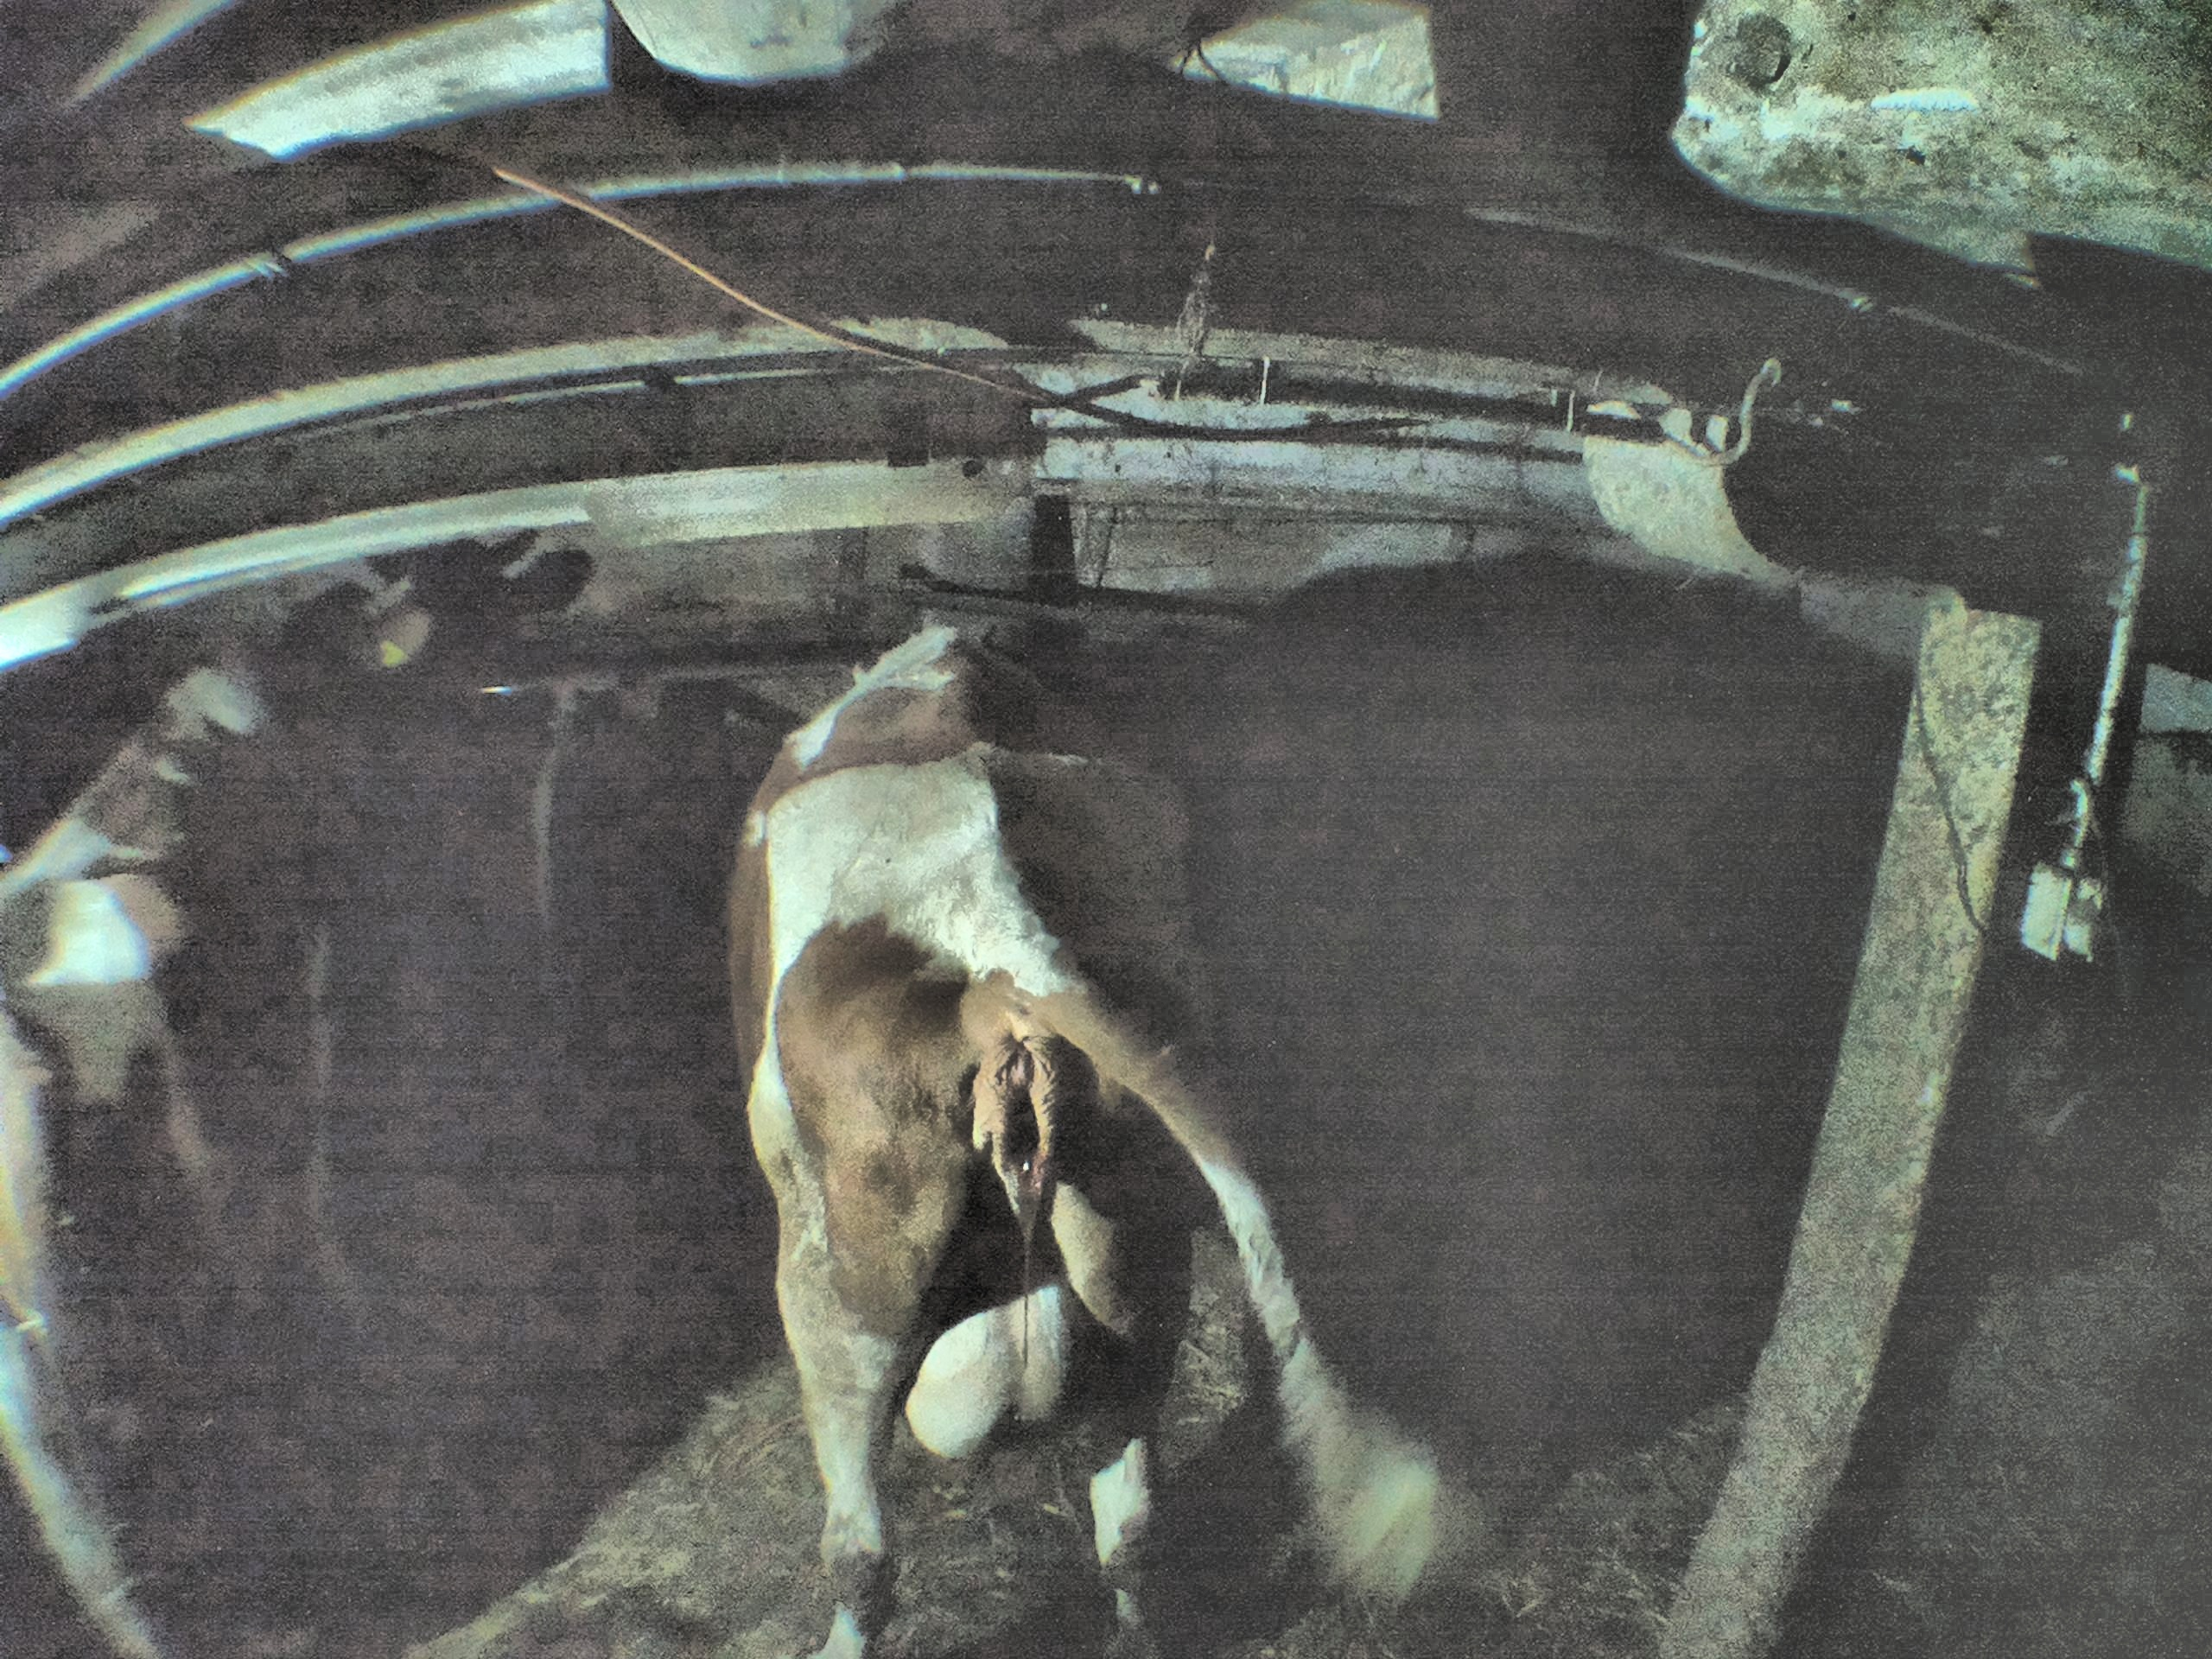
\includegraphics[scale=0.075]{Grafiken/schleimvagina.jpg}
	\caption{Schleim im Schambereich der Kuh kurz vor der Geburt} 
	\label{fig: Schleim im Schambereich der Kuh kurz vor der Geburt}
\end{figure}


\begin{figure}[h]
	\center
	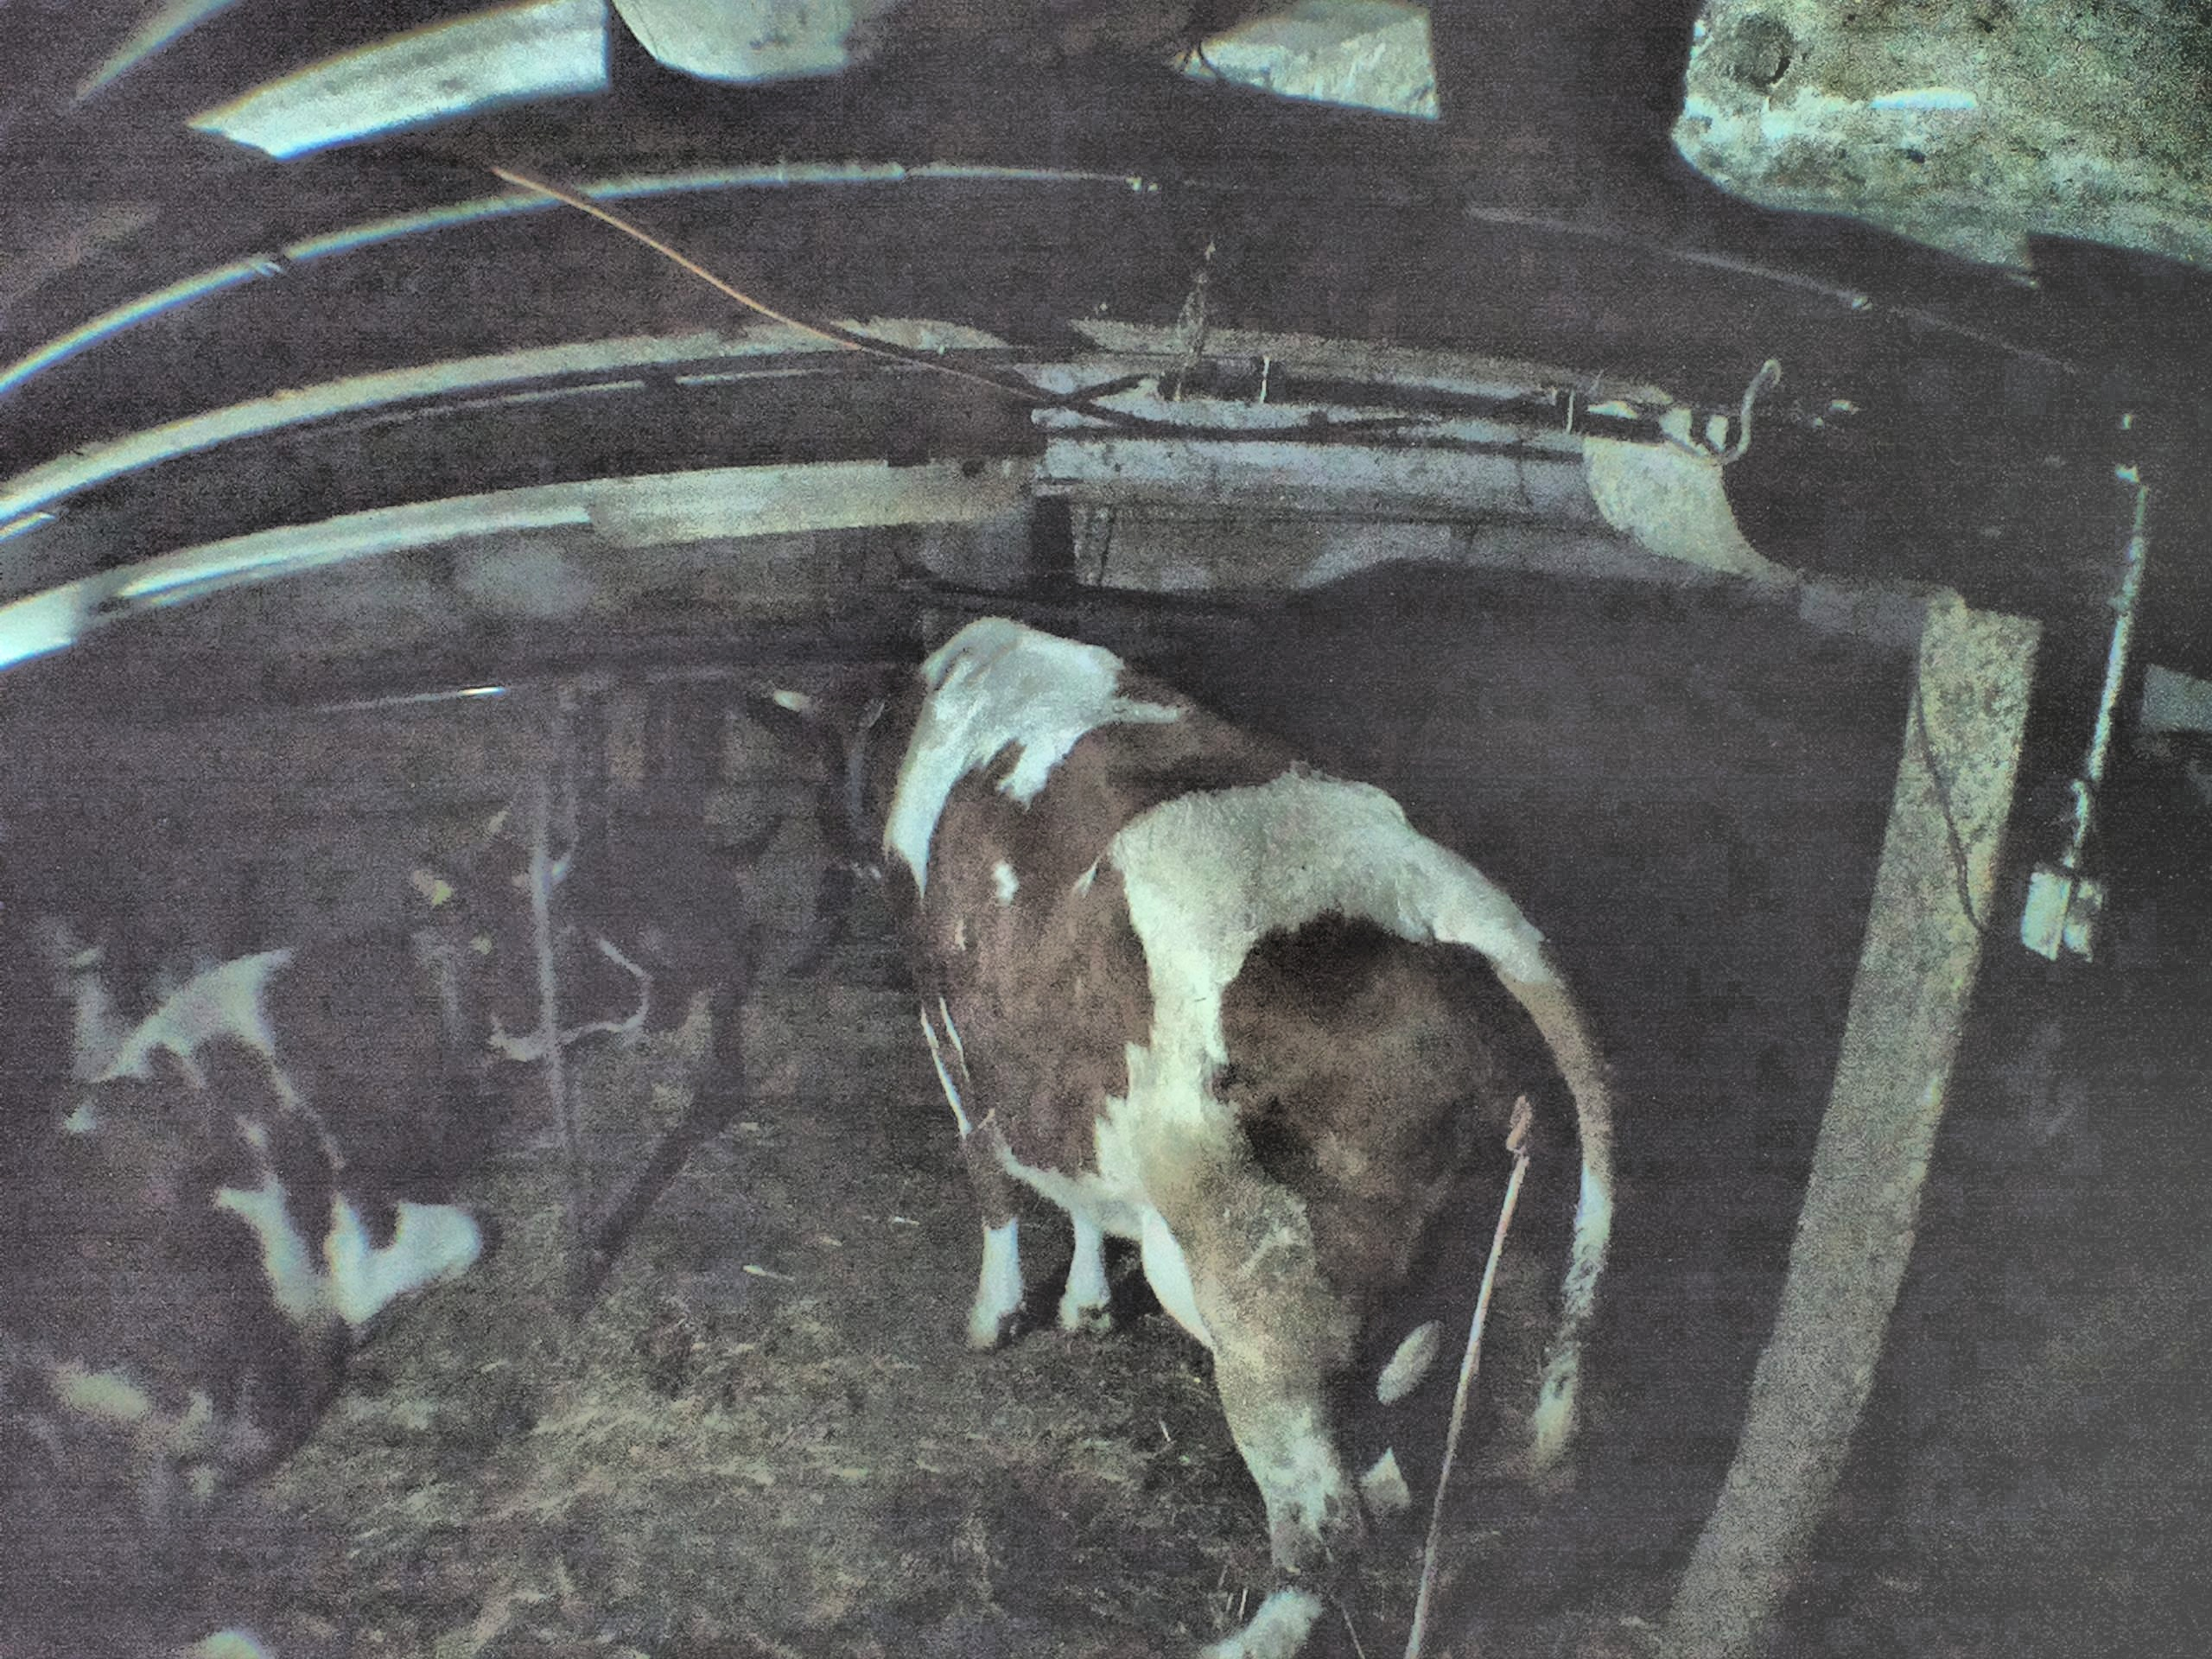
\includegraphics[scale=0.075]{Grafiken/schleim.jpg}
	\caption{Auslösung der Nachgeburt} 
	\label{fig: Auslösung der Nachgeburt}
\end{figure}  
	% ================================================================
% CHAPTER 3: Domänenanalyse: Domänenmodell
% ================================================================



\section{Domänenmodell}
\subsection{Legende zu den Diagrammen}
\begin{table}[H]
	\centering	
	\rowcolors{2}{maroon!10}{white!100}
	\arrayrulecolor{darkmaroon} 
	
	\begin{tabular}{ p{2cm}  p{12cm}  }
		
		\toprule[1pt]
		\rowcolor{maroon!30}	
		Farbe & Beschreibung \\
		
		\midrule
Grün \cellcolor[RGB]{204,235,197}&  Biologische Gegenstände im Domänenmodell und Value Objects in der Bibliothek, welche diese natürlichen Gegenstände beschreiben. \\
Lila \cellcolor[RGB]{253,218,236} & Zu optimierende Ressourcen und Faktoren und Value Objects in der Bibliothek,  welche diese zu optimierenden Gegenstände beschreiben.\\
Blau\cellcolor[RGB]{179,205,227} &  Objekte oder Resultate der Domäne \flqq{}Image Analysis\frqq{}. Zudem Value Objects in der Bibliothek, welche die Gegenstände dieser Domäne beschreiben. \\
Braun \cellcolor[RGB]{229,216,189}& Tatsächlicher Kern der Domäne \flqq{}Image Analysis\frqq{}. Dieser Kern implementiert das wichtigste Domänenwissen und zentrale Funktionen.\\			
Violett \cellcolor[RGB]{222,203,228} & Objekte, die zum Versenden von Benachrichtigungen benötigt werden und Value Objects in der Bibliothek, welche die Gegenstände dieser Domäne beschreiben.\\
Grau\cellcolor[RGB]{242,242,242} &  Paket für die Konfiguration der Benachrichtigungen und Value Objects in der Bibliothek, welche die Gegenstände dieser Domäne beschreiben.\\		
Gelb \cellcolor[RGB]{255,255,204}& Value Objects, welche direkt im Domänenmodell oder in der Lösungsdokumentation eingebettet sind. Zudem Value Objects die nicht kategorisiert werden können, da diese in mehreren Paketen eingesetzt werden. \\		
Orange \cellcolor[RGB]{254,217,166} &  Paket Housekeeping und Klassen vom Paket \flqq{}Image Analysis\frqq{}, welche dem Housekeeping dienen. \\
		
		\bottomrule
		
	\end{tabular}
	\caption{Legende fürs Domänenmodell und für die UML-Diagramme als Lösungsdokumentation}
	\label{tab: Legende fürs Domänenmodell und für die UML-Diagramme als Lösungsdokumentation}
\end{table}

\newgeometry{margin=2.5cm} % Ränder kleiner	
\begin{landscape}

\subsection{Domänenmodell Geburt}
\begin{figure}[H]
	\center
	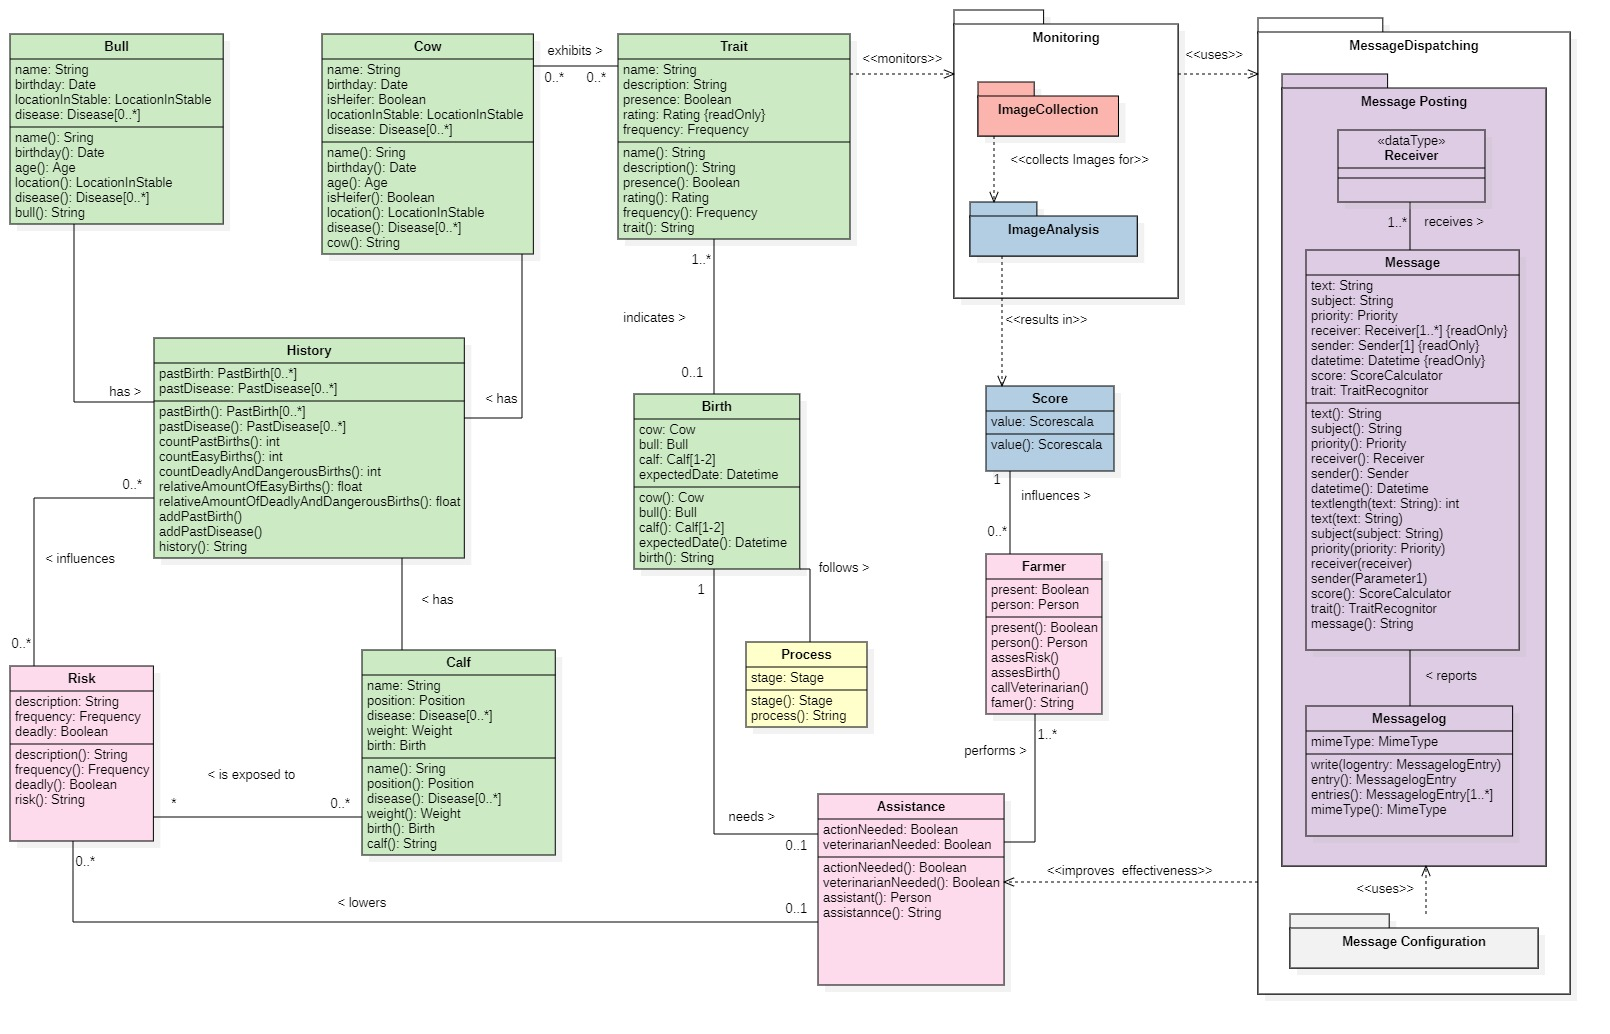
\includegraphics[scale=0.38]{Grafiken/modelle/domain-birth.jpg}
	\caption{Domänenmodell Kalbsgeburt} 
	\label{fig: Domänenmodell Kalbsgeburt}
\end{figure}


\subsection{Allgemeine Bibliothek an Value Objects }
\begin{figure}[H]
	\center
	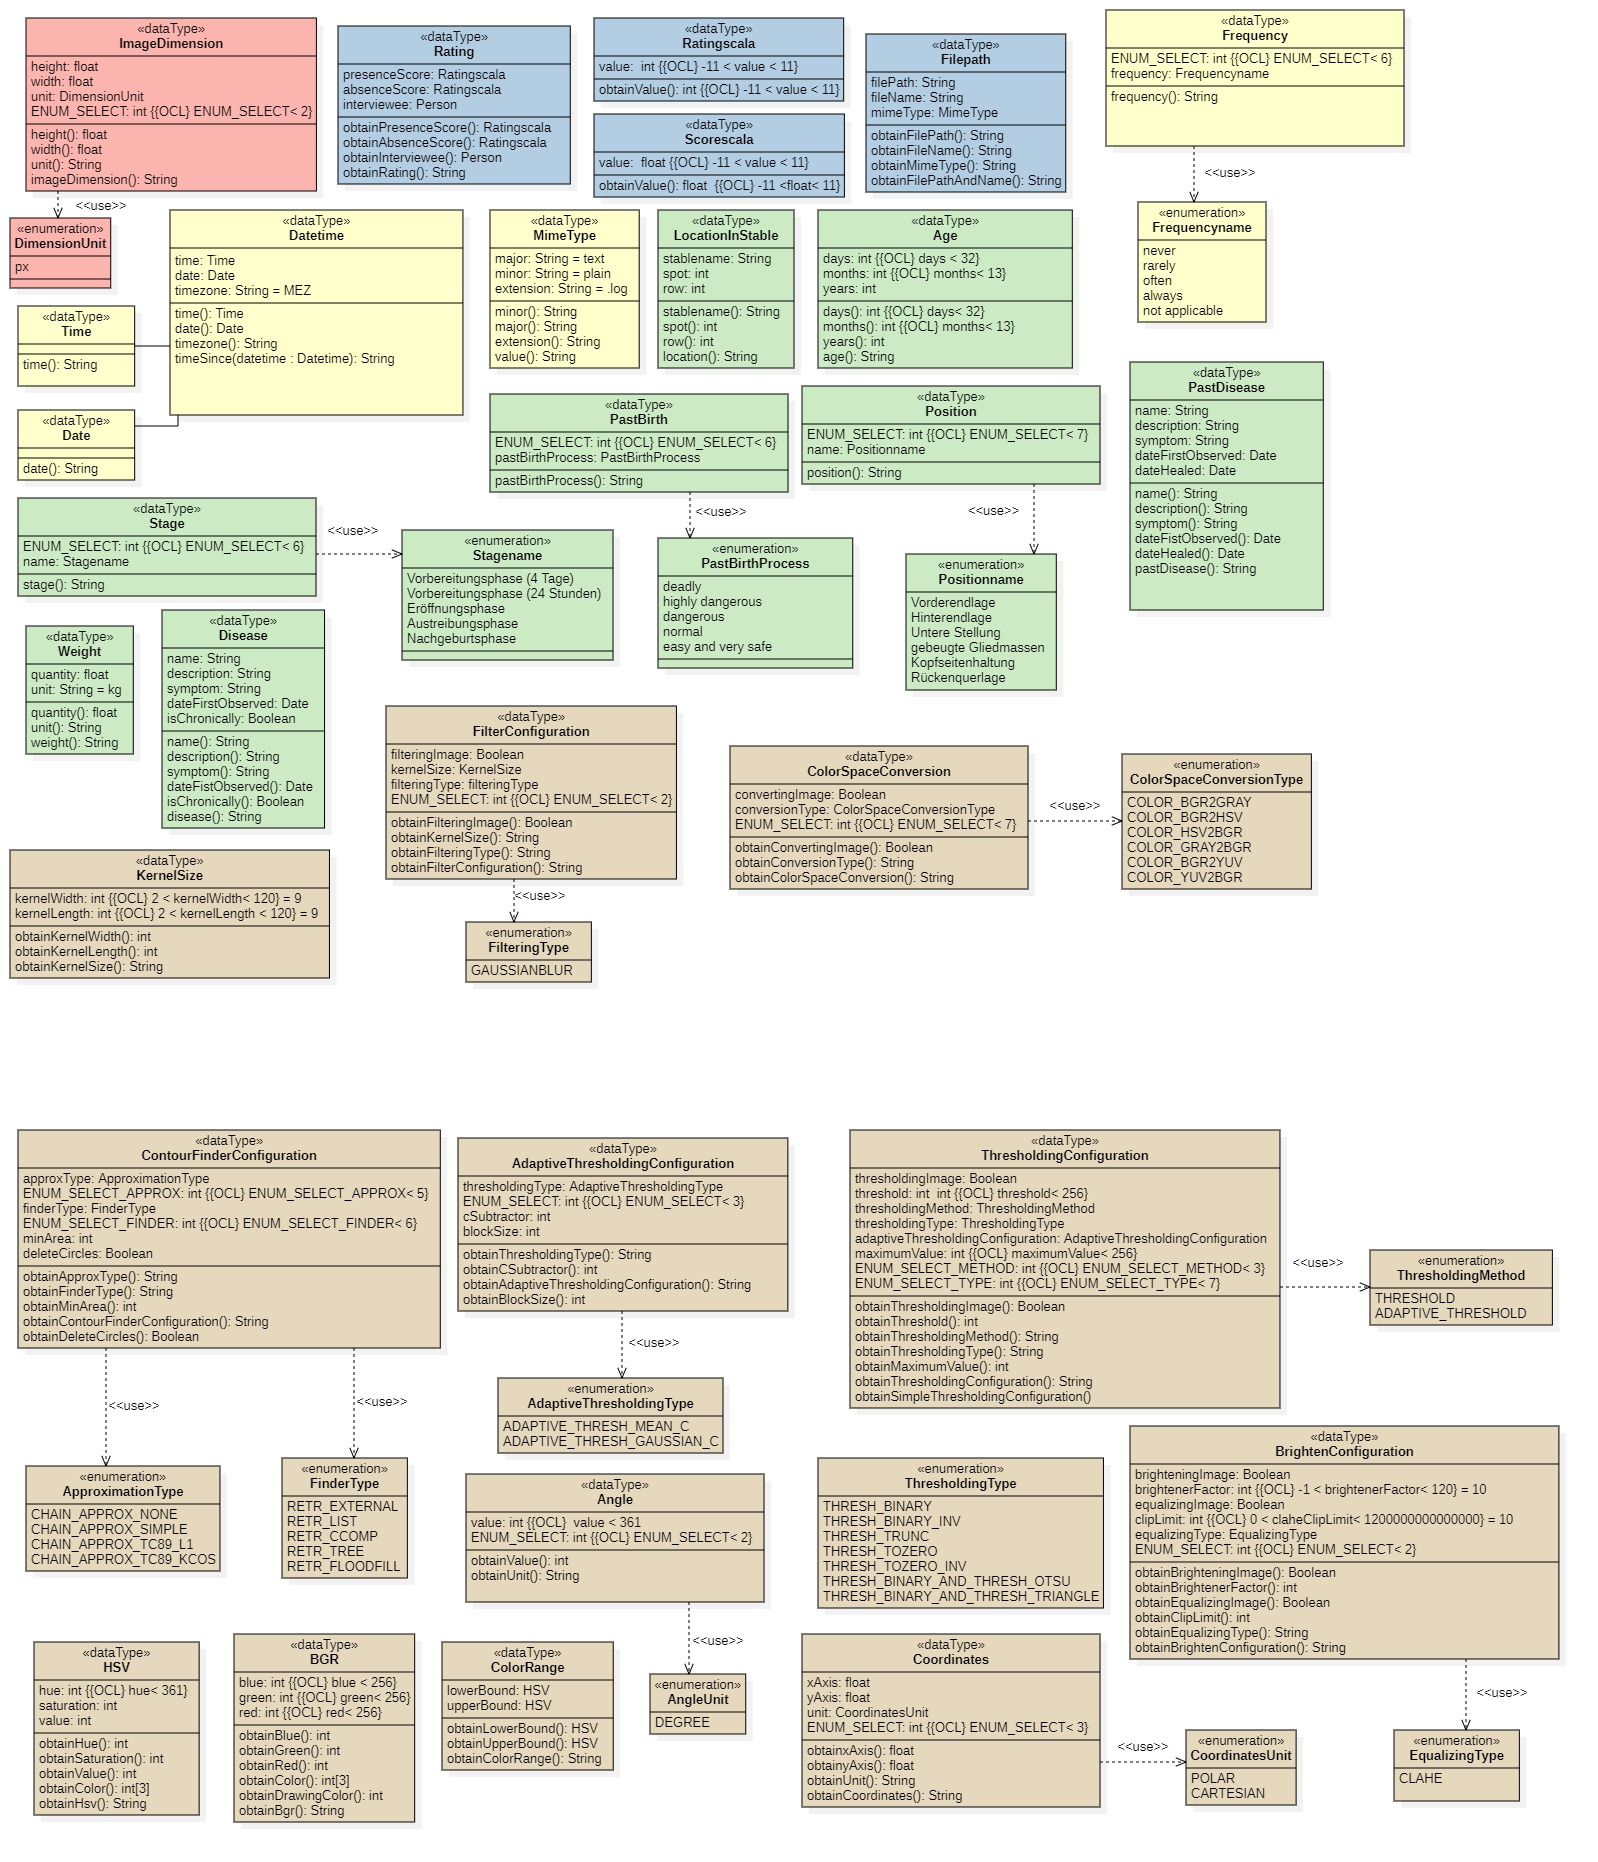
\includegraphics[scale=0.4]{Grafiken/modelle/vo-general.jpg}
	\caption{Allgemeine Bibliothek an Value Objects} 
	\label{fig: Allgemeine Bibliothek an Value Objects}
\end{figure}

\subsection{Bibliothek an Value Objects zur Konfiguration und zum Versand von Nachrichten}
\begin{figure}[H]
	\center
	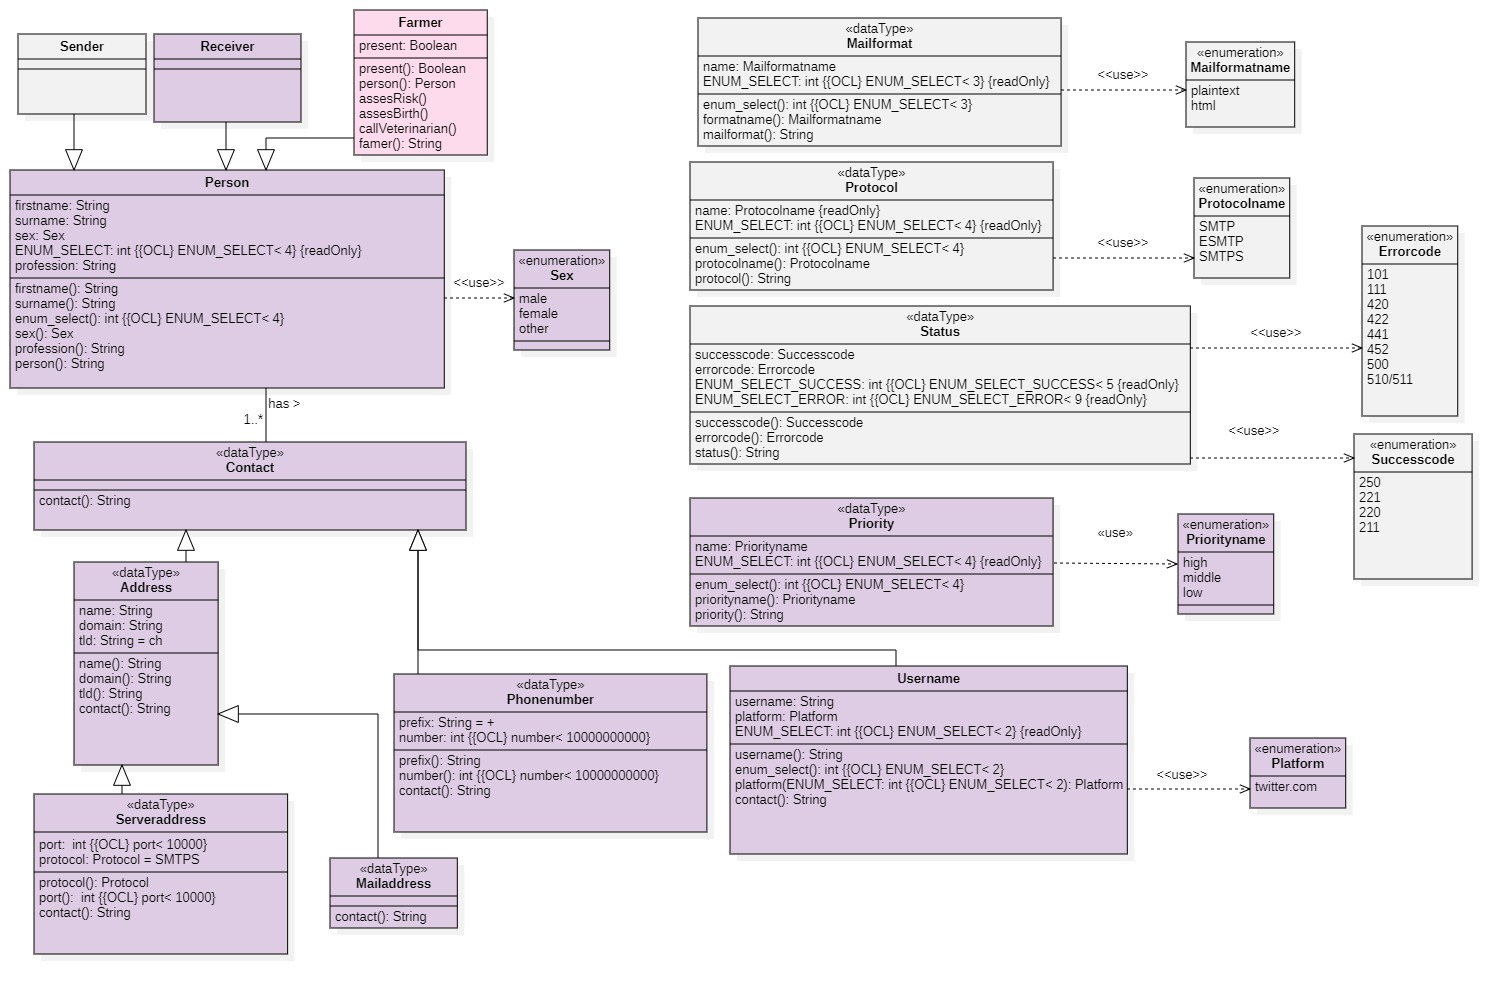
\includegraphics[scale=0.38]{Grafiken/modelle/vo-messaging.jpg}
	\caption{Bibliothek an Value Objects bezüglich Konfiguration und Versand von Nachrichten} 
	\label{fig: Bibliothek an Value Objects zur Konfiguration und zum Versand von Nachrichten}
\end{figure}


\end{landscape}
\restoregeometry % Wieder die alten Ränder                              
	% ================================================================
% CHAPTER 4: Lösung
% ================================================================

	
\chapter{Lösung}

\section{Codierung von Domänenwissen}

Die Tabellen \ref{tab: Bewertung der Anwesenheit und Abwesenheit von Merkmalen} bis \ref{tab: Zuordnung und Bewertung der Häufigkeiten von Merkmalen (Gaby Hirsbrunner)} und  codieren Domänenwissen von Tierärzten, welches für die Geburtsprognose von Bedeutung ist. Expertenwissen ist so codiert, dass jedes Geburtsmerkmal mit einer Gewichtung versehen ist. Somit hat das Merkmal an Stelle $i$ die Gewichtung $\lambda_{i}$ und $x_{i}$ markiert ihre Anwesenheit ($x_i = 1$) oder Abwesenheit ($x_i = 0$).



Wie in Formel \ref{Linerarkombination zur Geburtsprognose} abgebildet, werden bei Erkennung eines oder mehrerer Merkmale in einem Bild, die Gewichtungen dieser Merkmale addiert. Merkmale, welche als Geburtsanzeichen dienen, haben eine positive Gewichtung und erhöhen dadurch das Endergebnis. Merkmale, welche darauf hinweisen, dass zurzeit keine Entbindung stattfindet, haben eine negative Gewichtung und senken das Endergebnis.


Das Resultat dieser Berechnung bezeichnet der Autor als \flqq qualitative Situationsbewertung\frqq. Diese wird mit einem Schwellwert verglichen, um zu entscheiden, ob eine Benachrichtigung verschickt wird.

Dabei kann die qualitative Situationsbewertung anhand der folgenden Linearkombination ermittelt werden: 



\begin{equation}\label{Linerarkombination zur Geburtsprognose}
v = h(x) = \sum_{i=1}^n \lambda_{i}*x_{i}
\end{equation}

 
Wobei $\lambda_{i}$ sich aus der fachlichen Gewichtung $\kappa_{i}$ und der technischen Qualitätsbeurteilung $\beta_{i}$ zusammensetzt. Die Skala zur Bewertung reicht von -10 bis 10, daher ergibt sich $ \lambda, \kappa, \beta   \: \varepsilon \: m =\:   \{ \:  m \: | \:  m \:  \varepsilon \:  \mathbb{Z}, -10 \:  \leq \: m \: \leq \:  10\} $.

Die fachliche Gewichtung eines Merkmals entspricht der Bewertung  der Stärke des Hinweises in Bezug auf eine bevorstehende Geburt. Dementsprechend codiert $\kappa$ Domänenwissen von Tierärzten zur merkmalsbezogene Einschätzung und Prognose des Geburtsverlaufs.

Die technische Qualitätsbeurteilung basiert auf der Güte der technischen Mittel zwecks Analyse der An- oder Abwesenheit eines Merkmals $x_{i}$ in einem Bild. Dementsprechend wird $\beta$ benötigt, weil nicht sämtliche Merkmale mit derselben Qualität auf deren An- oder Abwesenheit überprüft werden können.

Zwischen den beiden Gewichtungen $\kappa$ und $\beta$ existiert eine schwache Beziehung. Dies wird dadurch begründet, dass technische Zuverlässigkeit die Anwesenheit eines Merkmals nicht überbewerten soll. Beispielsweise soll eine besonders hohe technische Qualitätsbeurteilung und eine tiefe fachliche Gewichtung nicht in einer hohen Gewichtung resultieren. Um diese zwei Gewichtungen schwach miteinander in Beziehung zu setzen, werden diese addiert und nicht multipliziert. Es gilt also: $\lambda_{i} = \kappa_{i} + \beta_{i}$

Die Variable  $x_{i}$ codiert die Anwesenheit ($x_{i}=1$) oder die Abwesenheit ($x_{i}=0$) eines spezifischen Merkmals auf einem Bild. Es gilt dementsprechend  $ x_{i} \:  \varepsilon \: \{0,1\}. $ 


Setzen wir diese Erkenntnisse zusammen, so ergibt sich

\begin{equation}\label{Vollständige Linerarkombination zur Geburtsprognose}
v = h(x) = \sum_{i=1}^n (\kappa_{i}+\beta_{i}) *x_{i}
\end{equation}

wobei:  $ x \:  \varepsilon \: \{0,1\} $ und $ \lambda, \kappa, \beta   \: \varepsilon \: m =\: \{ \:  m \: | \:  m \:  \varepsilon \:  \mathbb{Z}, -10 \:  \leq \: m \: \leq \:  10\} $.

Das Ergebnis dieser Rechenoperation ergibt wie bereits erwähnt die qualitative Situationsbewertung $v$, welche anhand der Indikatorfunktion $g$ mittels eines Schwellwertes ausgewertet wird» . Dies wird formal wie folgt ausgedrückt:

\begin{equation}\label{Vollständige Linerarkombination zur Geburtsprognose: Schwellwertanalyse}
y = g(v) =\begin{cases}
			1,\: wenn \: v > q\\
			0,\: wenn \: v \leq q
\end{cases}
\end{equation}

Dabei steht $q$ für den Schwellwert, welcher in der Domänenanalyse ermittelt wird. Das Ergebnis $y=1$ bedeutet, dass eine Benachrichtigung ausgelöst wird, während bei $y=0$ keine Benachrichtigung ausgelöst wird.

 






\newgeometry{margin=2.5cm} % Ränder kleiner	
\begin{landscape}

\section{Modellierung der Lösung}
Für die Dokumentation der Lösung verwendet der Autor die UML-Notation. Bei der Modellierung werden Empfehlungen aus dem Buch \flqq{}UML 2 glasklar\frqq{} \cite{Uml-modellierung2012} berücksichtigt. 

\subsection{Klassendiagramm des Pakets Image-Analysis }
\begin{figure}[H]
	\center
	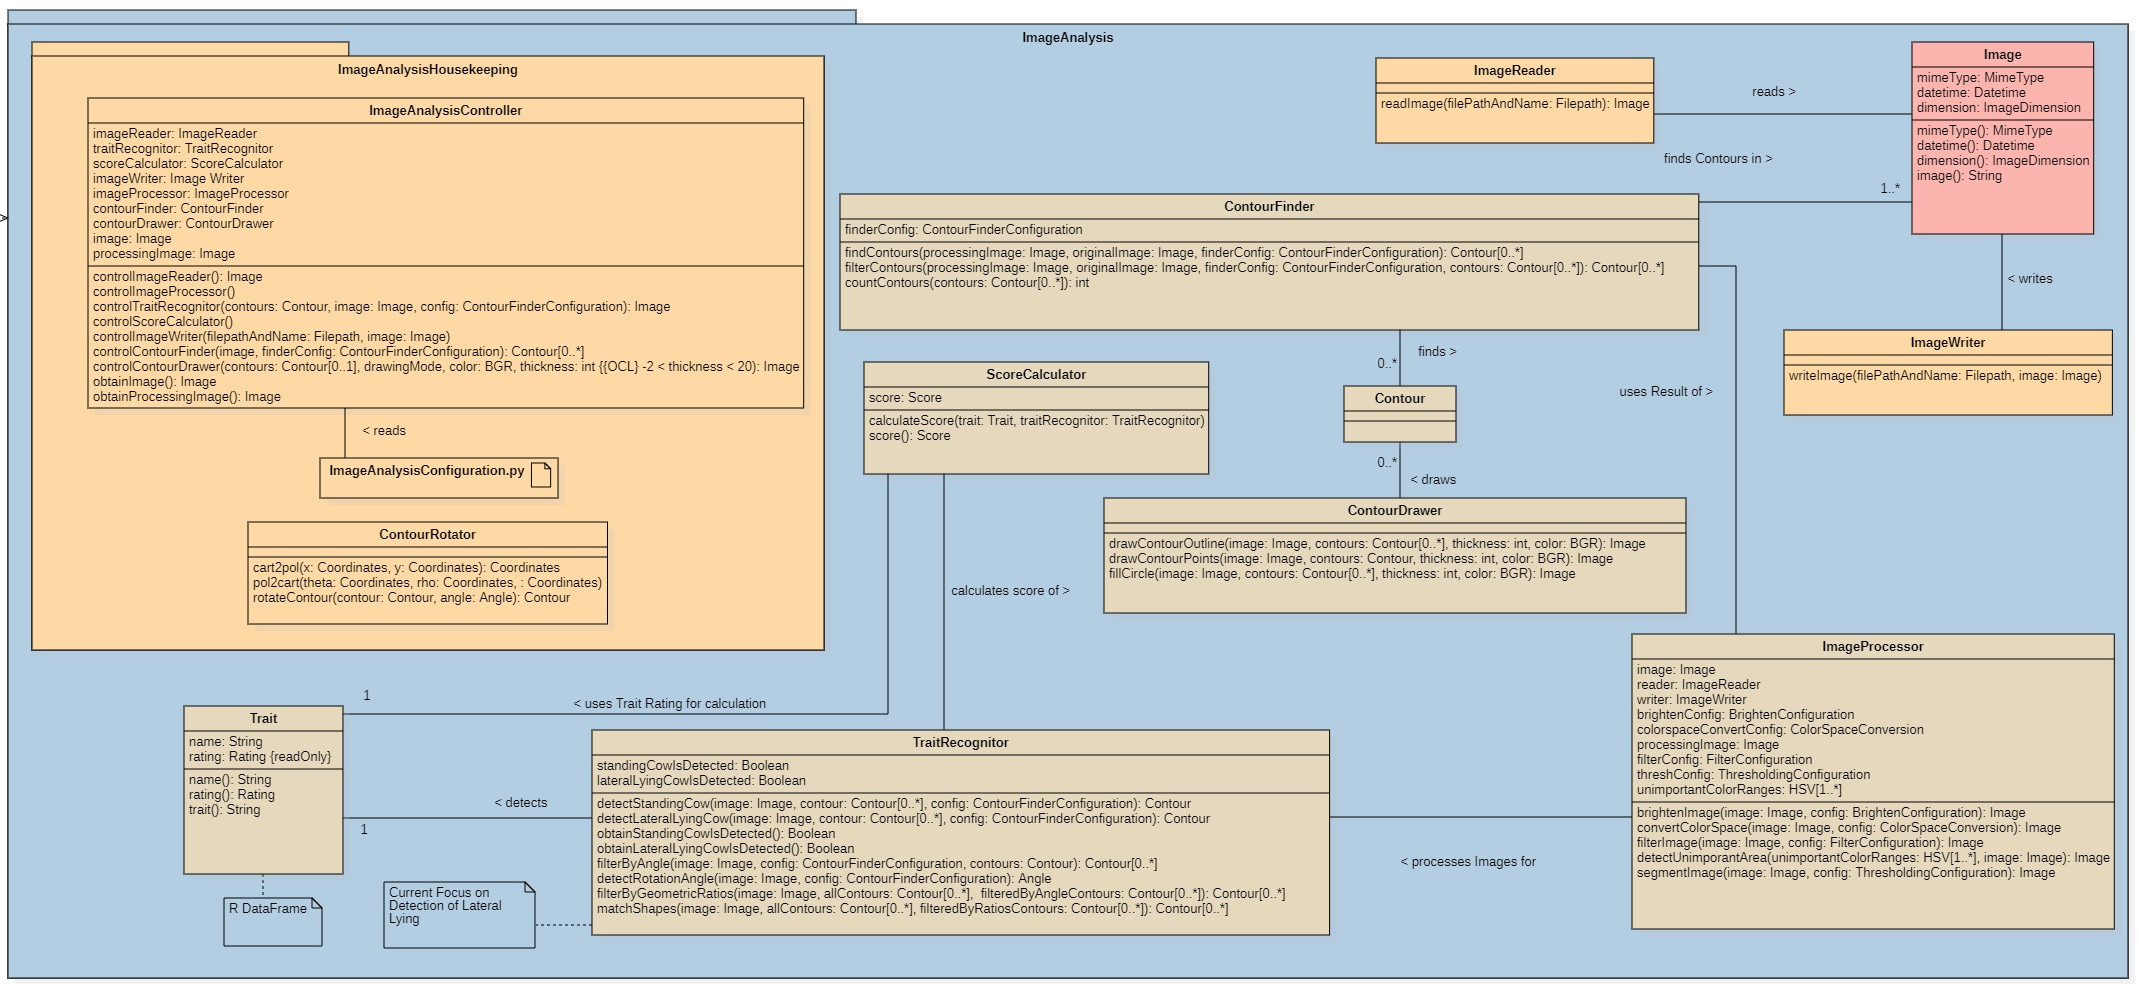
\includegraphics[scale=1.35]{Grafiken/modelle/solution-imageanalysis-1.jpg}
	\caption{Lösungsdokumentation des Pakets Image-Analysis zur Geburtsprognose und Geburtserkennung.} 
	\label{fig: Lösungsdokumentation des Pakets Image-Analysis zur Geburtsprognose und Geburtserkennung.}
\end{figure}

\subsection{Klassendiagramm der Pakete Message-Configuration und Message-Posting}
\begin{figure}[H]
	\center
	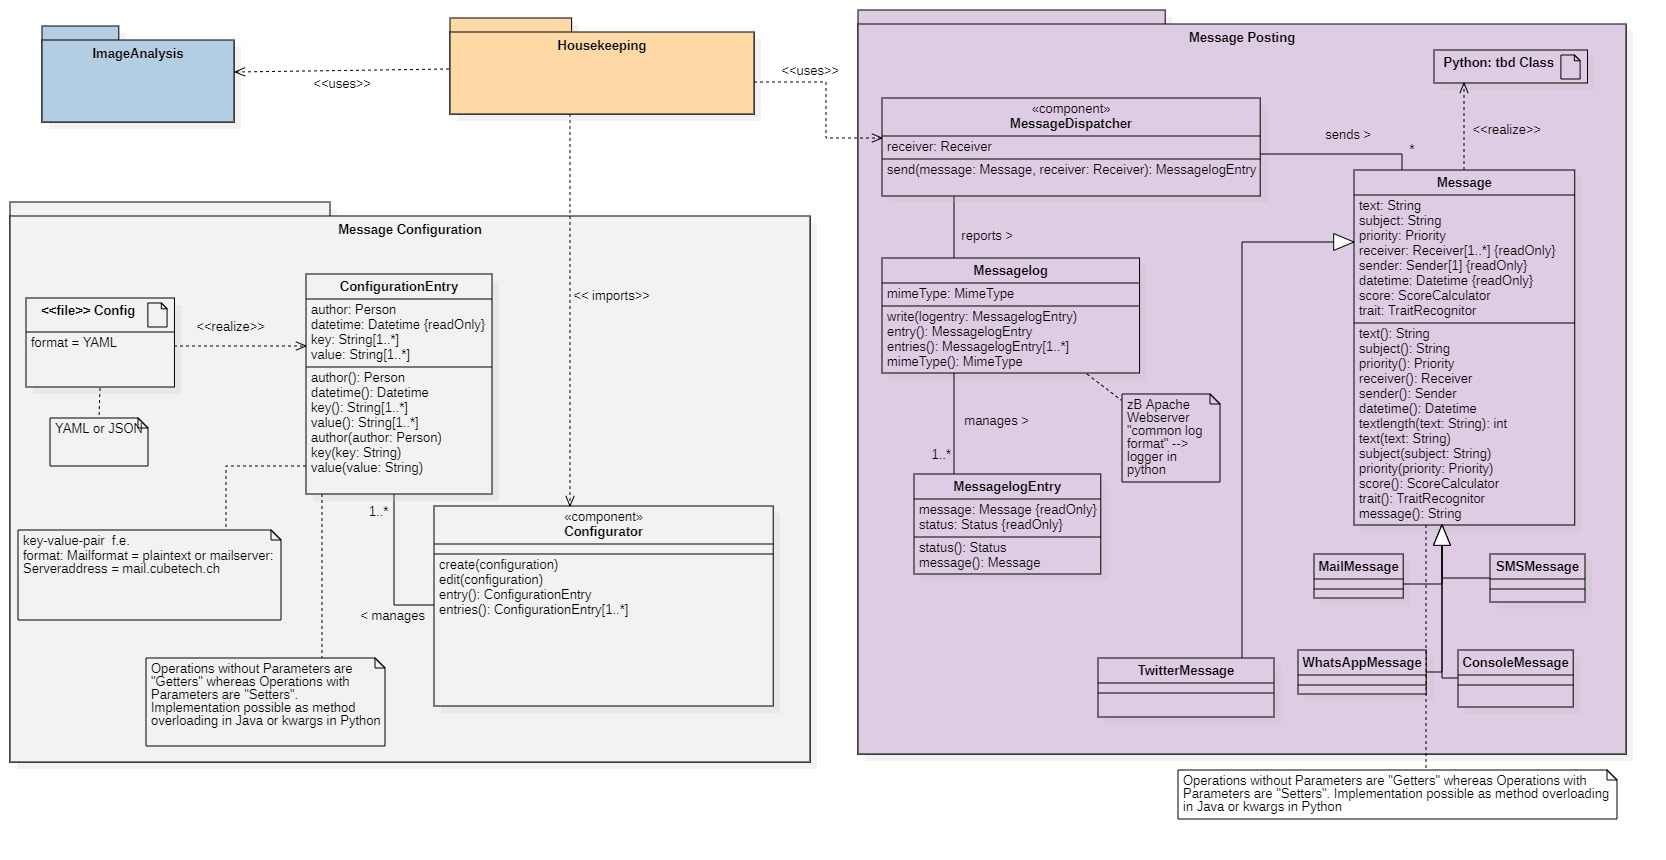
\includegraphics[scale=0.43]{Grafiken/modelle/solution-messaging.jpg}
	\caption{Lösungsdokumentation der Pakete Message-Configuration zur Konfiguration und Message Posting zum Versand von Benachrichtigungen.} 
	\label{fig: Lösungsdokumentation der Pakete Message-Configuration zur Konfiguration und Message Posting zum Versand von Benachrichtigungen.}
\end{figure}


\end{landscape}
\restoregeometry % Wieder die alten Ränder


\section{Umsetzung in Entwicklung}
Für Bildanalysen sind grundsätzlich Methoden des Machine Learning geeignet. Da für die vorliegende Arbeit jedoch nicht auf eine grosse Menge von klassifizierten Bildern zugegriffen werden kann, wird die Bildanalyse auf Basis von geometrischen Eigenschaften durchgeführt.
Um die schrittweise Entwicklung und entsprechende Teilergebnisse der Bildbearbeitung zu veranschaulichen, dient Abbildung \ref{fig: Ausgangslage für die Bildanalyse} als Ausgangsbild. Dieses Bild wurde vom System erstellt, welches im Rahmen der erwähnten Case-Arbeit entwickelt wurde. Anschliessend wurde das Bild mit der Funktion \texttt{add()} heller gemacht und unter Anwendung von \texttt{createCLAHE()} und \texttt{clahe.apply()} wurde das Histogramm des Bildes geglättet. 

\begin{figure}[H]
	\center
	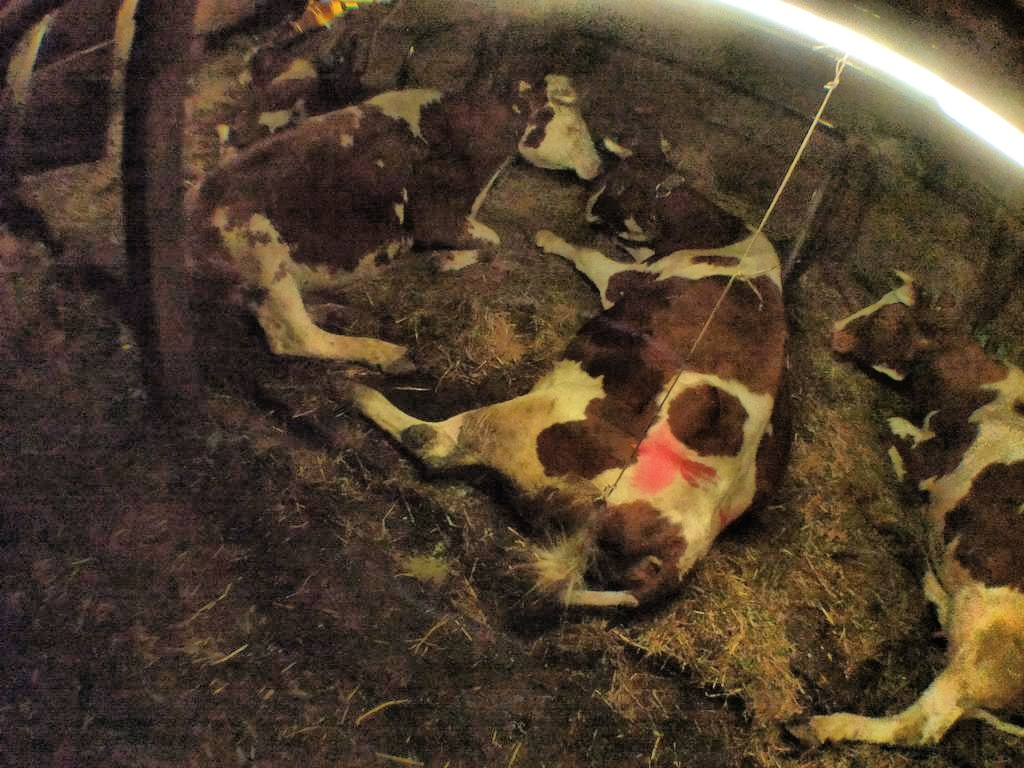
\includegraphics[scale=0.43]{Grafiken/entwicklung/1ausgangsbildBericht.jpg}
	\caption{Beispielbild als Ausgangslage zur Veranschaulichung des Vorgehens} 
	\label{fig: Ausgangslage für die Bildanalyse}
\end{figure}

Abbildung \ref{fig: Vergleich der Histogramme vor und nach Bildbearbeitung} zeigt auf der linken Seite das Histogramm des Originalbilds und auf der rechten Seite das Histrogramm des aufgehellten und geglätteten Bilds. Dabei fällt auf, dass aufgrund der Aufhellung des gesamten Bildes im Histogramm der Wertebereich nach rechts verschoben wird. Zudem sind als Folge der Glättung des Histogramms mittels CLAHE\footnote{Contrast Limited Adaptive Histogram Equalization} die Anzahl Pixel weniger stark auf einen Bereich konzentriert. CLAHE ist ein Verfahren, dass für die Glättung von Bildern und Verbesserung des Kontrasts eingesetzt wird. Ein Vorteil der Methode ist, dass aufgrund einer parametrisierbaren Begrenzung der Kontrastverstärkung die Überbetonung von Rausch in relativ homogenen Regionen des Bilds verhindert wird \citep[S. 313]{FernandezVillan2019}.

Das Bild \ref{fig: Ausgangslage für die Bildanalyse} wird nun unter Anwendung von diversen Methoden aus der Bildanalyse und der Software-Bibliothek OpenCV bearbeitet und analysiert, um daraus Informationen zum Geburtsverlauf eines Kalbes zu gewinnen. In der vorliegenden Arbeit liegt der Fokus in der Detektierung von seitlichem Liegen, da die Erkennung dieses Geburtsmerkmals einen hohen Mehrwert bringt. 

\begin{figure}[H]
	\center
	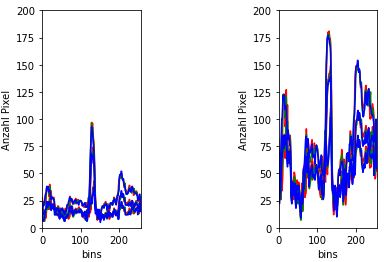
\includegraphics[scale=0.9]{Grafiken/entwicklung/2HistrogrammVergleich.jpg}
	\caption{Vergleich der Histogramme vor und nach Bildbearbeitung} 
	\label{fig: Vergleich der Histogramme vor und nach Bildbearbeitung}
\end{figure}

\subsection{Detektierung von unwichtigen Bereichen im Bild}
Um das Potential aus der Detektierung von unwichtigen Bereichen zu veranschaulichen, wird in einem ersten Schritt ein Binärbild des Originalbilds erstellt. Dazu wird die Funktion \texttt{threshold()} mit dem Verfahrentyp \texttt{THRESH_BINARY} und dem Wert \texttt{90} als Schwellwert eingesetzt. OpenCV ermöglicht mit der Funktion \texttt{threshold()}, die Segmentierung des Bilds. Dabei wird dieses in eine Repräsentation umgewandelt, welche sich für die Weiterverarbeitung besser eignet als die ursprüngliche. \cite[S.328-335]{FernandezVillan2019} In der vorliegenden Arbeit basiert die Extraktion von Objekten darauf, dass durch Schwellwertverfahren bestimmte Eigenschaften wie Farben und Ecken erkannt werden können und dadurch mittels Parition des Bildes zwischen Vorder- und Hintergrund unterschieden werden kann. Die Auswahl vom Wert \texttt{90} als Schwellwert hat zur Folge, dass Pixel mit einer Intensität kleiner gleich \texttt{90} im resultierenden Bild schwarz dargestellt werden und alle anderen Pixel weiss. Gleichung \ref{Schwellwertanalyse} verdeutlicht die Folge der Parametrisierung von \texttt{threshold()} in der vorliegenden Arbeit. 

\begin{equation}\label{Schwellwertanalyse}
dst(x,y) =\begin{cases}
255,\: if \: src(x,y) > 90\\
0\: otherwise
\end{cases}
\end{equation}

Als Bild zur Eingabe dient ein Graustufenbild. Grundsätzlich können mithilfe des Parameters \texttt{maxval} bei Erreichung des Schwellwerts auch Graustufen als Zielwert für Pixel zugewiesen werden. Da in der vorliegenden Arbeit das Schwellwertverfahren aber in erster Linie zur Vorbereitung für \texttt{findContours()} gemacht wird, bringt ein Bild in Graustufen keinen Mehrwert. Die Funktion \texttt{findContours()} weist sämtlichen Pixeln, die nicht den Wert \texttt{0} haben, den Wert \texttt{1} zu. Dementsprechend wird auch ein Bild mit Graustufen als Binärbild behandelt \cite[S. 366]{FernandezVillan2019}. 



Nebst der Funktion \texttt{threshold()} und dem Typ \texttt{THRESH_BINARY} bietet OpenCV weiteren Typen wie \texttt{THRESH_BINARY_INV} oder \texttt{THRESH_TRUNC} und das adaptive Schwellwertverfahren \texttt{adaptiveThreshold()} an. Adaptive Schwellwertverfahren ermöglichen den Einsatz von spezifischen Schwellwerten für einen Pixel im Zielbild. Dieser spezifische Schwellwert wird auf Basis einer Gruppe von benachbarten Pixeln  ermittelt \cite[S.342 f]{FernandezVillan2019}. Die im Rahmen der Bachlor-Arbeit entwickelte Lösung unterstützt die Parametrisierung dieser Funktionen mittels Enumerations. Diese haben für die vorliegende Bildanalyse jedoch keine zentrale Bedeutung und werden deshalb nicht weiter erläutert.

\begin{figure}[H]
	\center
	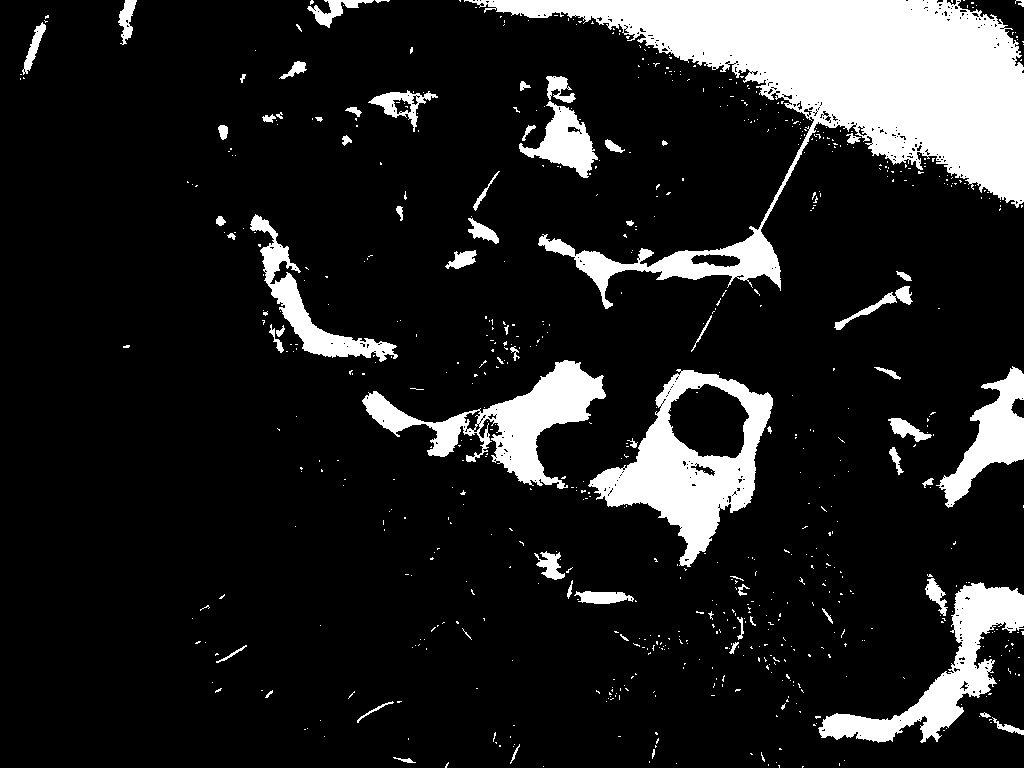
\includegraphics[scale=0.43]{Grafiken/entwicklung/8thresholdedMask.jpg}
	\caption{Binärbild als Resultat vom Schwellwertverfahren} 
		\label{fig: Binärbild als Resultat vom Schwellwertverfahren}
\end{figure}
		
Im Binärbild aus Abbildung \ref{fig: Binärbild als Resultat vom Schwellwertverfahren} werden anschliessend mit den Funktionen \texttt{findContours()} und \texttt{drawContours()} Konturen gesucht und im Originalbild eingezeichnet. Die Funktion \texttt{findContours()} wird verwendet, um Konturen in einem Binärbild zu erkennen. Der Algorithmus unterstützt unterschiedliche Modi wie \texttt{RETR_EXTERNAL} für die Beschränkung auf äussere Konturen, \texttt{RETR_LIST} für die Ausgabe sämtlicher Konturen ohne Hierarchie oder \texttt{RETR_TREE} für die zusätzliche Ausgabe von Informationen zur Hierarchie der Konturen \cite[S.366]{FernandezVillan2019}. In der vorliegenden Arbeit wurde in erster Linie der Verfahrenstyp \texttt{RETR_EXTERNAL} verwendet. Abweichungen werden entsprechend erwähnt.

\begin{figure}[H]
	\center
	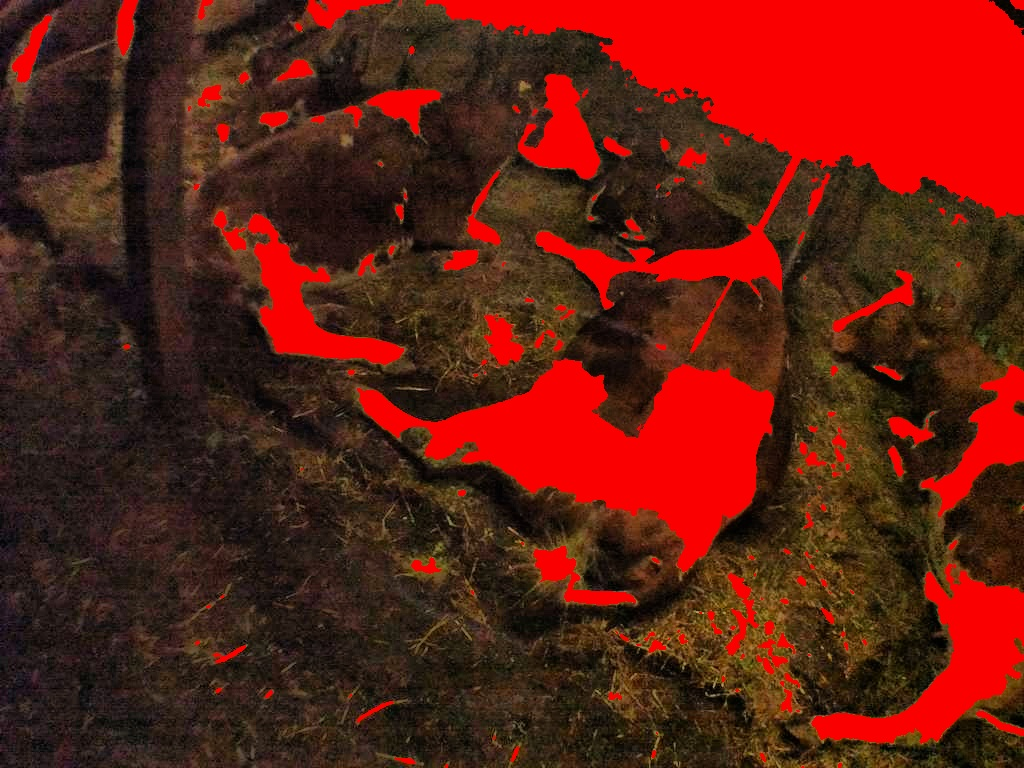
\includegraphics[scale=0.43]{Grafiken/entwicklung/8thresholdedImageAllContours.jpg}
	\caption{Originalbild mit sämtlichen Konturen rot eingefärbt} 
	\label{fig:Originalbild mit sämtlichen Konturen rot eingefärbt } 
\end{figure}

Die Anwendung der Funktion \texttt{findContours()} ohne Einschränkung der zu analysierenden Bereiche in Abbildung \ref{fig:Originalbild mit sämtlichen Konturen rot eingefärbt} verdeutlicht, dass viele Konturen eingezeichnet werden, die sich von den Konturen der Kuh stark unterscheiden. Im vorliegenden Bild betrifft dies in erster Linie die Lampe und Strohhaufen. Der Autor setzt sich daher zum Ziel, unwichtige Bereiche im Bild zu identifizieren. Dies umfasst Bereiche, welche mit hoher Wahrscheinlichkeit nicht Teile einer Kuh oder eines Kalbs zeigen. Die Farbwerte dieser Teile im Bild
unterscheiden sich stark von den meisten Farben im Kuhfell. 

Die Strohhaufen und Schatten unterhalb des Schwanzes oder unterhalb der Beine der Kuh werden ganz einfach gefiltert, indem nur Konturen mit einer Fläche von mehr als 1250 Pixel berücksichtigt werden. Daraus entsteht Abbildung \ref{fig:Originalbild mit rot eingefärbten Konturen, falls Fläche über 1250 Pixel}.

\begin{figure}[H]
	\center
	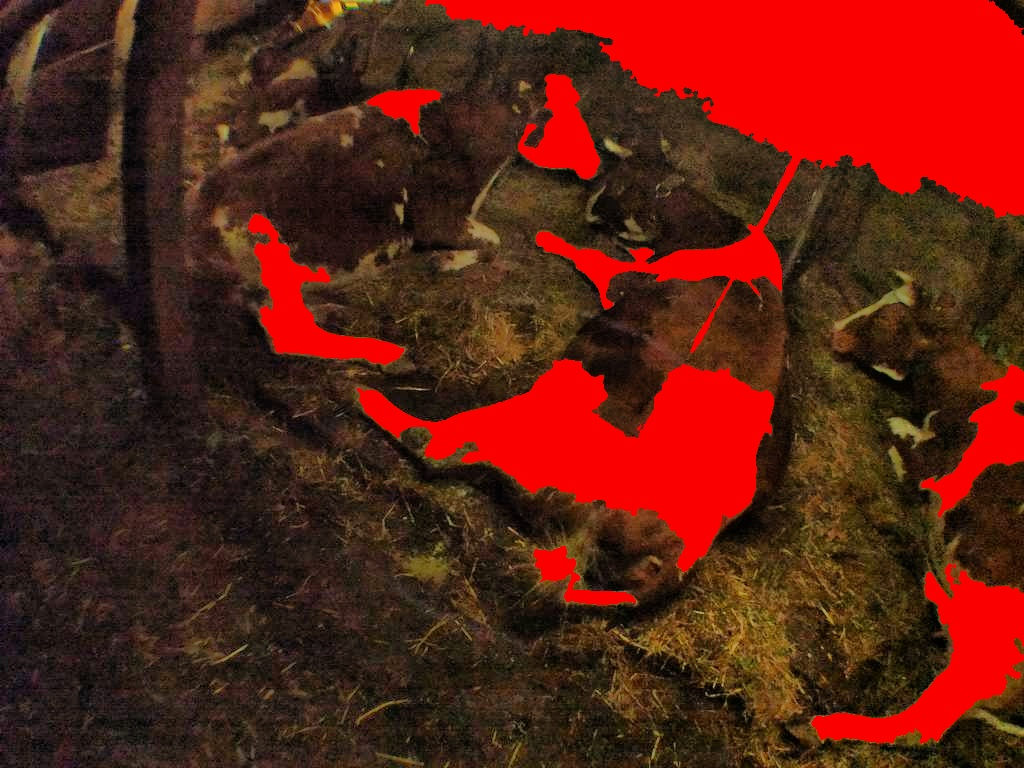
\includegraphics[scale=0.43]{Grafiken/entwicklung/9thresholdedImage.jpg}
	\caption{Originalbild mit rot eingefärbten Konturen mit Fläche über 1250 Pixel} 
	\label{fig:Originalbild mit rot eingefärbten Konturen, falls Fläche über 1250 Pixel} 
\end{figure}

Um weitere, unwichtige Konturen wie die Lampe zu erkennen, wird ein Verfahren zur Analyse von Farbwerten durchgeführt.
Dabei wird in einem ersten Schritt ein Farbbereich für die Lampe definiert. Um einen Richtwert für diesen Farbwert zu erhalten, wird mithilfe des Grafikprogramms GIMP (Version 2.10, \url{www.gimp.org}) ein Farbwert im Bereich der Lampe ausgelesen. Auf Basis dieses Richtwerts wird anschliessend ein Wertebereich für die Farbwerte der zu identifizierenden Lampe festgelegt. Diese Schwellwerte werden der Funktion \texttt{inRange()} von OpenCV zwecks Erstellung eines Binärbilds übergeben. Sämtliche Bereiche mit Farbwerten, die sich zwischen den definierten Schwellwerten befinden, werden im resultierenden Bild weiss dargestellt. Diese entsprechen unwichtigen Bereichen im Bild. Alle anderen Bereiche sind im erstellen Binärbild schwarz dargestellt. Abbildung \ref{fig: Binärbild stellt den Bereich der Lampe weiss dar} zeigt das Binärbild, welches aus diesem Verfahren entsteht. Es ist klar zu erkennen, dass die Bereiche der Lampe weiss und übrige Bereiche schwarz sind. Der Ansatz der Schnur, mit welcher der Schwanz der Kuh an der Decke befestigt wird, ist ebenfalls erkennbar. 




\begin{figure}[H]
	\center
	
\includegraphics[scale=0.25]{Grafiken/entwicklung/3binBildLampe.jpg}
	\caption{Binärbild stellt den Bereich der Lampe weiss dar} 
	\label{fig: Binärbild stellt den Bereich der Lampe weiss dar}
\end{figure}

Dasselbe Vorgehen wird angewendet, um den Bereich des Stallbodens und Holzträgers zu identifizieren. Das erstellte Binärbild identifiziert auch einige dunkle Regionen im Deckenbereich als unwichtig. Das Ergebnis ist in Abbildung \ref{fig: Binärbild zeigt den Bereich des Stallbodens und Holzträgers} abgebildet.
\begin{figure}[H]
	\center
	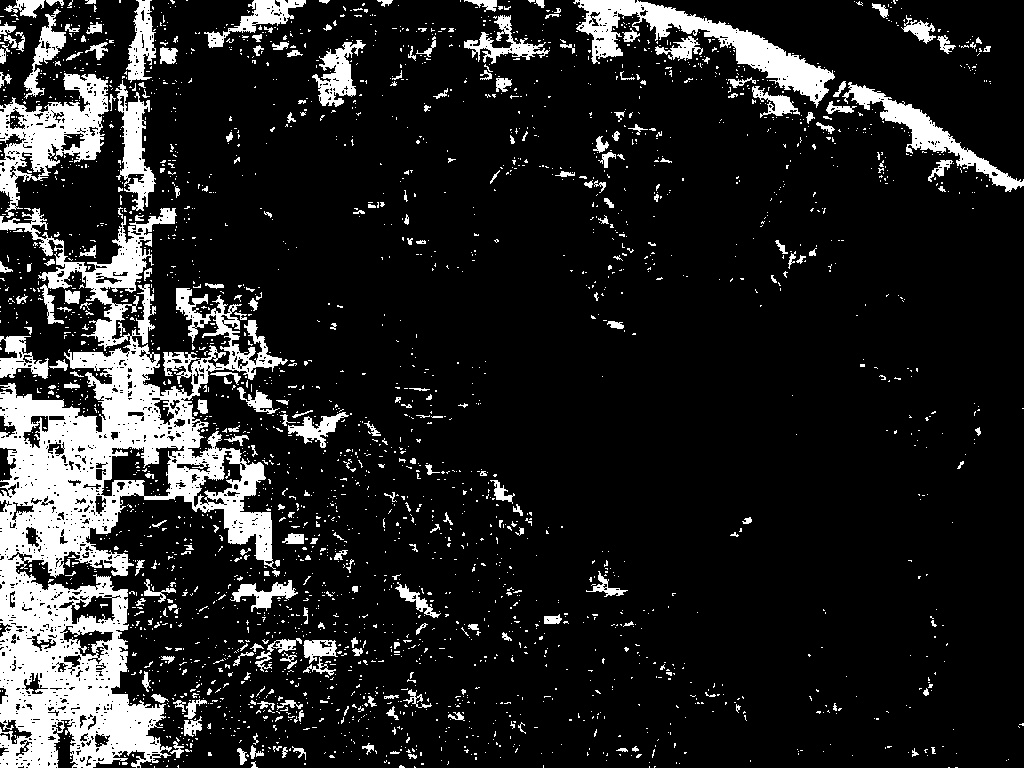
\includegraphics[scale=0.25]{Grafiken/entwicklung/4binBildHolz.jpg}
	\caption{Binärbild zeigt den Bereich des Stallbodens und Holzträgers} 
	\label{fig: Binärbild zeigt den Bereich des Stallbodens und Holzträgers}
\end{figure}

Diese zwei Binärbilder werden nun mit dem Ziel weiterverarbeitet, ein Binärbild zu erstellen, welches möglichst viele unwichtige Regionen weiss darstellt. Durch die Funktion \texttt{bitwise_or} werden die Bilder so verknüpft, dass im resultierenden Bild sämtliche Bereiche weiss sind, die in einem der beiden oder in beiden Eingangsbildern weiss sind.
\begin{figure}[H]
	\center
	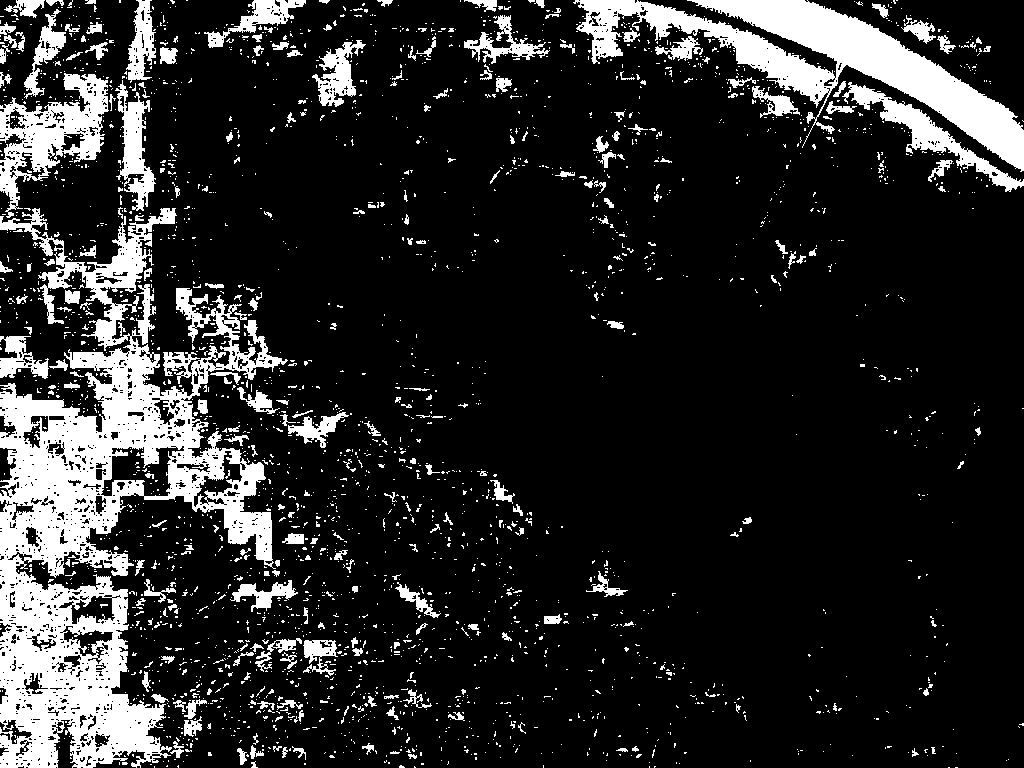
\includegraphics[scale=0.25]{Grafiken/entwicklung/5binLampeUndHolz.jpg}
	\caption{Binärbild zeigt die als unwichtig identifizierten Bereiche} 
	\label{fig: Binärbild zeigt sämtliche als unwichtig identifizierten Bereiche}
\end{figure}

Ausgehend von Abbildung \ref{fig: Binärbild zeigt sämtliche als unwichtig identifizierten Bereiche} können die als unwichtig identifizierten Bereiche als Konturen erkannt und im Originalbild eingezeichnet werden. Um dies zu erreichen, werden die Funktionen \texttt{findContours()} und \texttt{drawContours()} wie bereits erwähnt angewendet. Das Resultat ist in Abbildung \ref{fig: Unwichtige Bereiche als Konturen} veranschaulicht. 
\begin{figure}[H]
	\center
	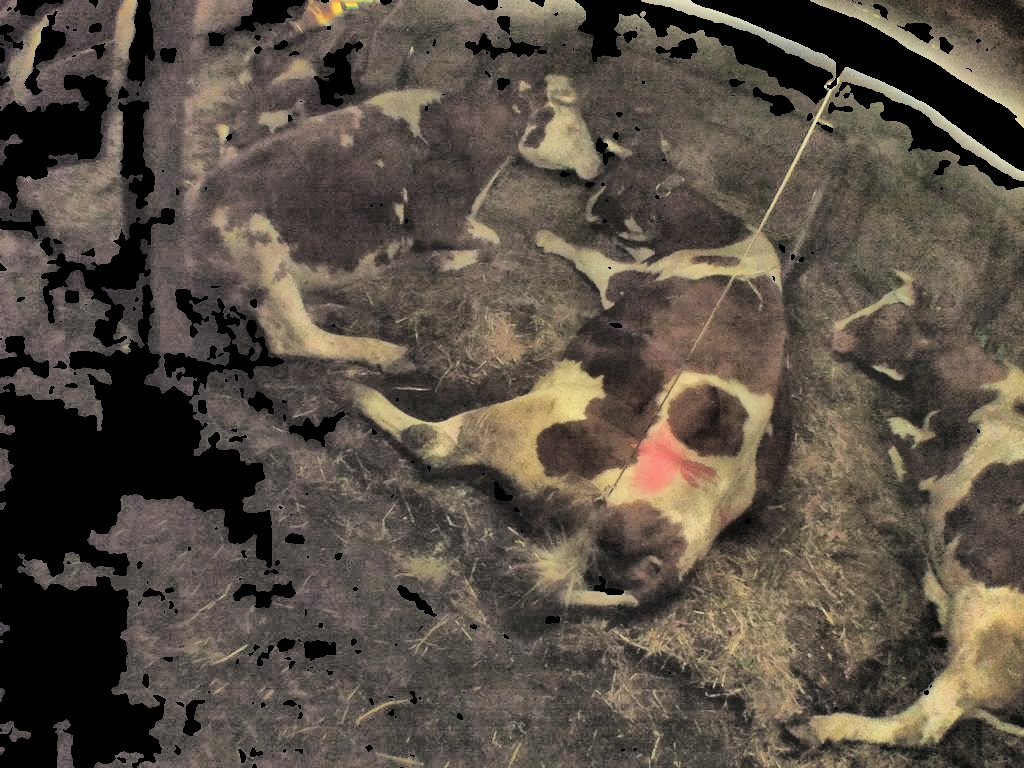
\includegraphics[scale=0.43]{Grafiken/entwicklung/6unwichtigeBereicheEingezeichnet.jpg}
	\caption{Unwichtige Bereiche  als Konturen} 
	\label{fig: Unwichtige Bereiche als Konturen}
\end{figure}

Nun gilt es, auf Basis der als unwichtig identifizierten Konturen möglichst grosse Flächen aus dem Originalbild zu entfernen, respektive möglichst grosse Flächen mit schwarzer Farbe zu füllen. Um dies zu erreichen, werden mehrere Verfahren getestet. Die Abbildungen  \ref{fig: Unwichtige Bereiche als Polygone} bis \ref{fig: Unwichtige Bereiche als Rechtecke} veranschaulichen die entsprechenden Resultate unter Verwendung von OpenCV. 

In Abbildung \ref{fig: Unwichtige Bereiche als Polygone} wurde \texttt{approxPolyDP()} verwendet, um basierend auf den Konturen ein Vieleck zu approximieren. Die Funktion arbeitet nach dem Douglas-Peucker-Algorithmus, welcher aus einer gegebenen Kontur eine dezimierte Kontur mit weniger Punkten erstellt. Dabei kann der Funktion die maximale Distanz der originalen Kontur und ihrer Approximation als Argument mitgegeben werden \citep[S. 383]{FernandezVillan2019}.  

\begin{figure}[H]
	\center
	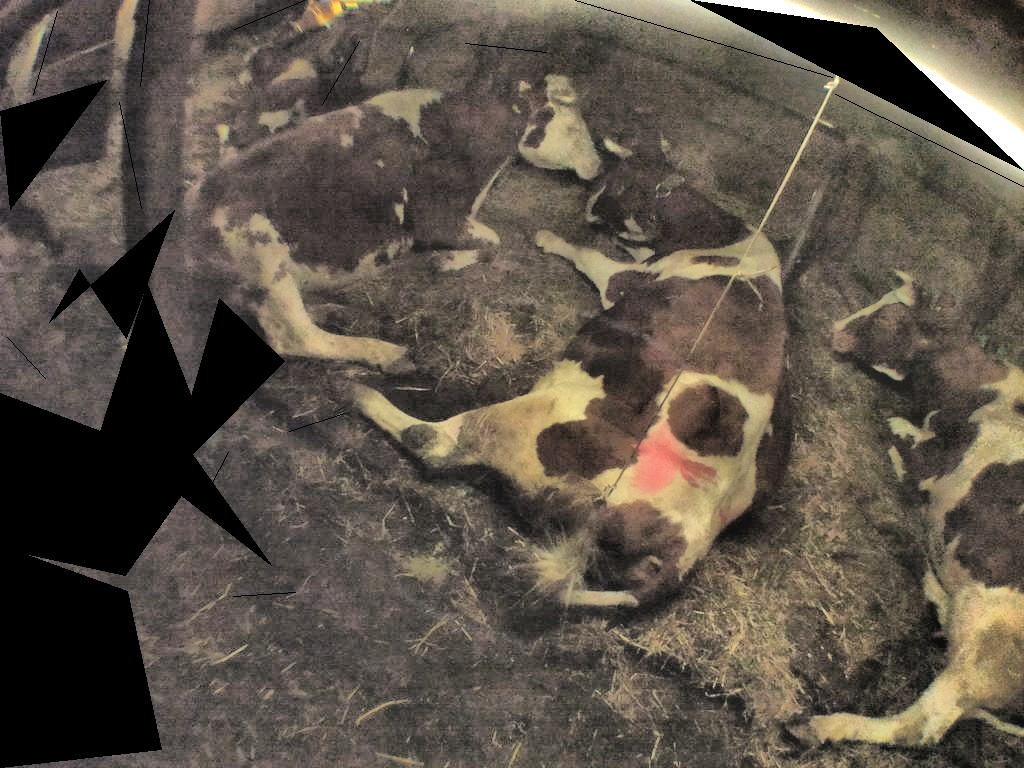
\includegraphics[scale=0.43]{Grafiken/entwicklung/7unwichtigePolygone.jpg}
	\caption{Unwichtige Bereiche als Polygone } 
	\label{fig: Unwichtige Bereiche als Polygone}
\end{figure}

Weiter wurde versucht, die unwichtige Fläche im Originalbild durch konvexe Hüllen zu maximieren. Das Bild \ref{fig: Unwichtige Bereiche als konvexe Hülle} zeigt konvexe Hüllen der Konturen,  die als Ergebnisse der Funktion \texttt{convexHull()} entstehen.

\begin{figure}[H]
	\center
	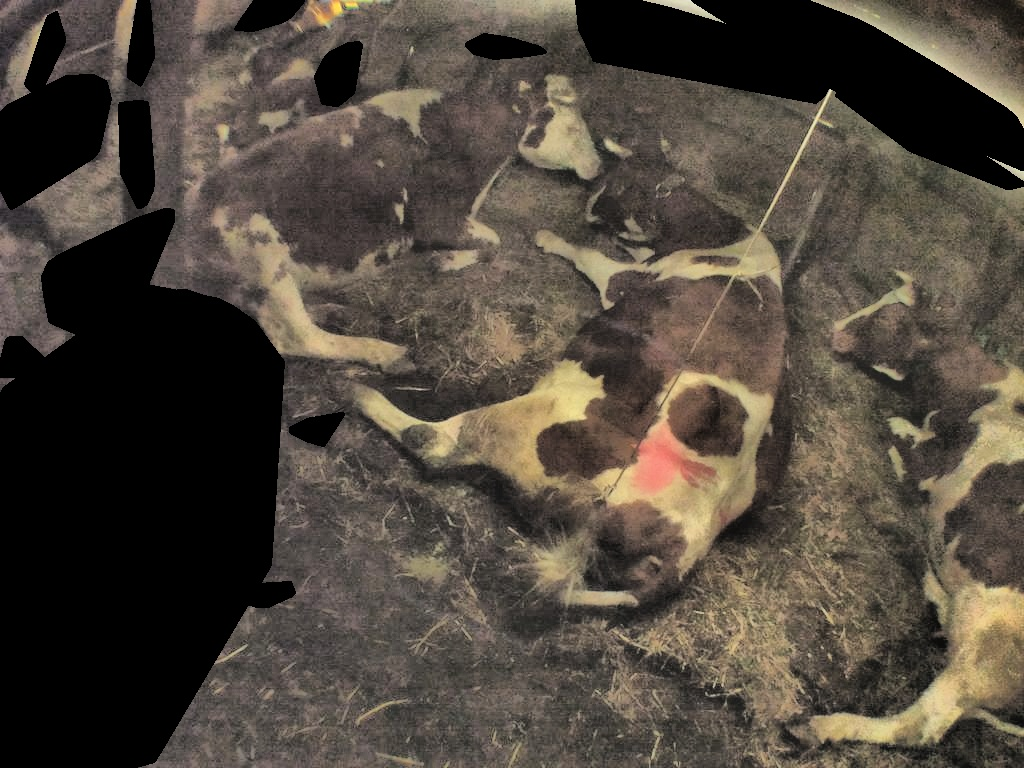
\includegraphics[scale=0.43]{Grafiken/entwicklung/7unwichtigeKonvexe.jpg}
	\caption{Unwichtige Bereiche als konvexe Hülle} 
	\label{fig: Unwichtige Bereiche als konvexe Hülle}
\end{figure}

 Als weiterer Lösungsansatz wurde die Funktion \texttt{minEnclosingCircle()} verwendet, um Kreise zu finden, welche Konturen mit möglichst geringer Fläche umschliessen (Abbildung \ref{fig: Unwichtige Bereiche als Kreise}).
 
\begin{figure}[H]
	\center
	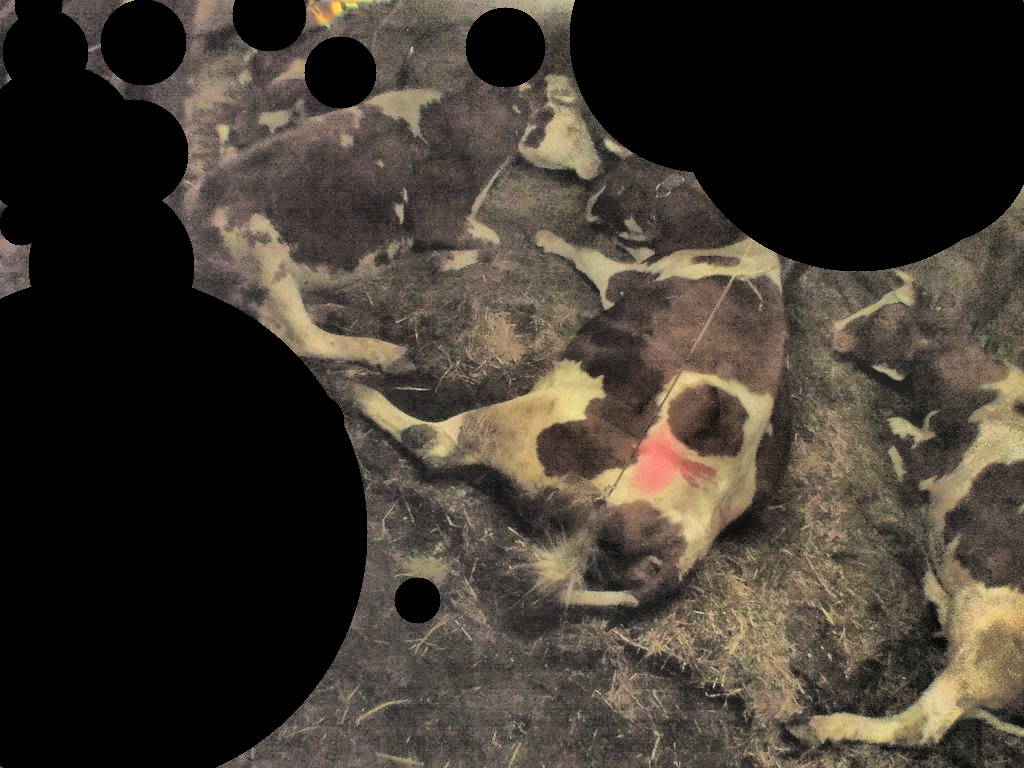
\includegraphics[scale=0.43]{Grafiken/entwicklung/7unwichtigeKreise.jpg}
	\caption{Unwichtige Bereiche als Kreise } 
	\label{fig: Unwichtige Bereiche als Kreise}
\end{figure}
Abschliessend wurden für die Abbildung \ref{fig: Unwichtige Bereiche als Rechtecke} mit der Funktion \texttt{boundingRect()} Rechtecke gebildet, welche die Konturen umschliessen.
\begin{figure}[H]
	\center
	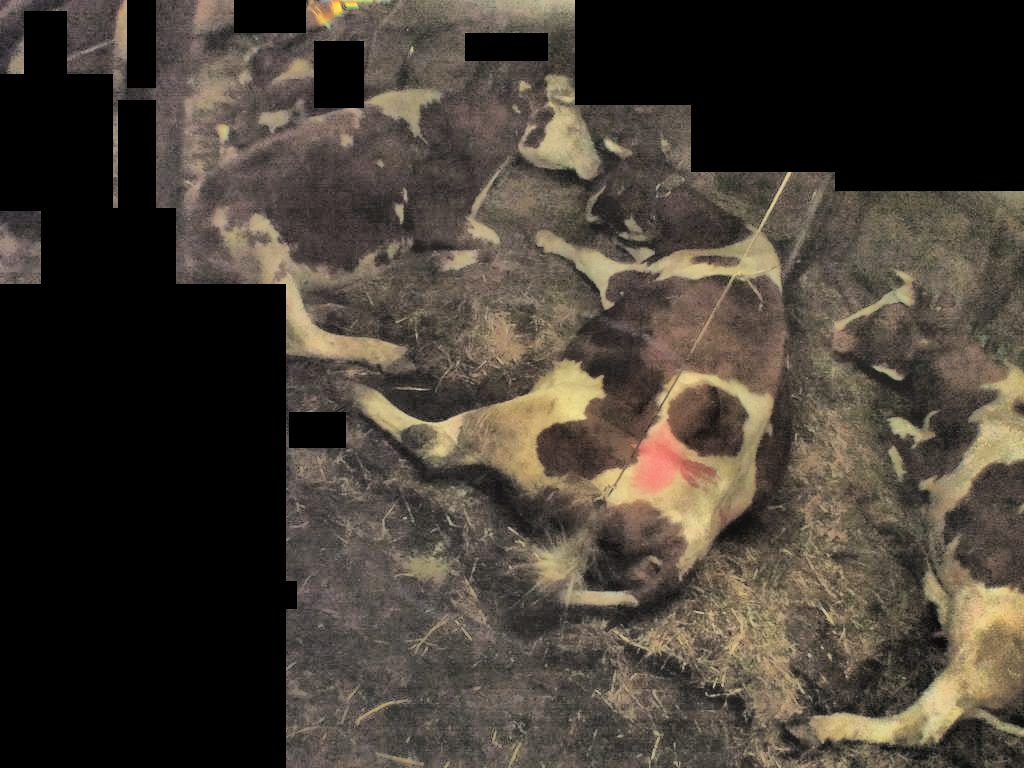
\includegraphics[scale=0.43]{Grafiken/entwicklung/7unwichtigeRechtecke.jpg}
	\caption{Unwichtige Bereiche als Rechtecke} 
	\label{fig: Unwichtige Bereiche als Rechtecke}
\end{figure}


Die Verfahren, welche mittels \texttt{minEnclosingCircle()} und \texttt{boundingRect()} angewendet werden, ergeben im vorliegenden Kontext die besten Ergebnisse. Einerseits werden die als unwichtig identifizierten Flächen  maximiert. Andererseits werden nur sehr kleine Bereiche der Kuh fälschlicherweise als unwichtig eingestuft. Da perfekte Kreise in nach der Ermittlung der Konturen mihilfe von \texttt{findContours()} bei den Kühen nicht vorkommen, entscheidet sich der Autor dafür, unwichtige Bereiche als schwarze Kreise einzuzeichnen. Zudem können diese Kreise in der weiteren Bildbearbeitung problemlos als solche erkannt werden.
Dementsprechend wird das in Abbildung \ref{fig: Unwichtige Bereiche als Kreise} dargestellte Bild zur weiteren Analyse verwendet.
An dieser Stelle ist jedoch auch Kritik an dieser Methode zur Bestimmung von unwichtigen Bereichen angebracht. Die Funktion \texttt{inRange()} benötigt einen Wertebereich für Farben, um die unwichtigen Bereiche zu finden. Dieser Wertebereich ist stark von den Lichtverhältnissen im untersuchten Bild abhängig. Bei Tests mit verschiedenen Bildern, die ebenfalls mit dem Rasperry Pi aufgenommen wurden, hat die falsche Detektierung von unwichtigen Bereichen das Gesamtergebnis verschlechtert. Aus diesem Grund wird mittels Konfiguration \texttt{AdvancedUnimportantColorRange=False} die Möglichkeit geboten, nur die Farbbereiche der Lampe zu nutzen. Diese wird in allen durchgeführten Tests zuverlässig detektiert.  
\subsection{Detektierung von wichtigen Bereichen im Bild}



In einem ersten Schritt wird die geglättete und aufgehellte Version von Bild \ref{fig: Unwichtige Bereiche als Kreise} mit dem adaptiven Schwellwertverfahren bearbeitet. Um dies zu erreichen, wird die Funktion \texttt{adaptiveThreshold()} mit den Argumenten \texttt{THRESH_BINARY_INV} und \texttt{ADAPTIVE_THRESH_MEAN_C} aufgerufen. Das Ergebnis dieses Versuchs, wichtige Bereiche des Bilds zu detektieren, ist in Abbildung \ref{fig: Detektierung von wichtigen Bereichen mittels adaptivem Schwellwertverfahren} ersichtlich. Die angestrebte Partitionierung des Bildes in Bereiche der Kuh und in alle anderen Bereiche funktioniert nicht. Deshalb wird der Versuch mit denselben Einstellungen aber mit einem nicht geglätteten Bild wiederholt.

\begin{figure}[H]
	\center
	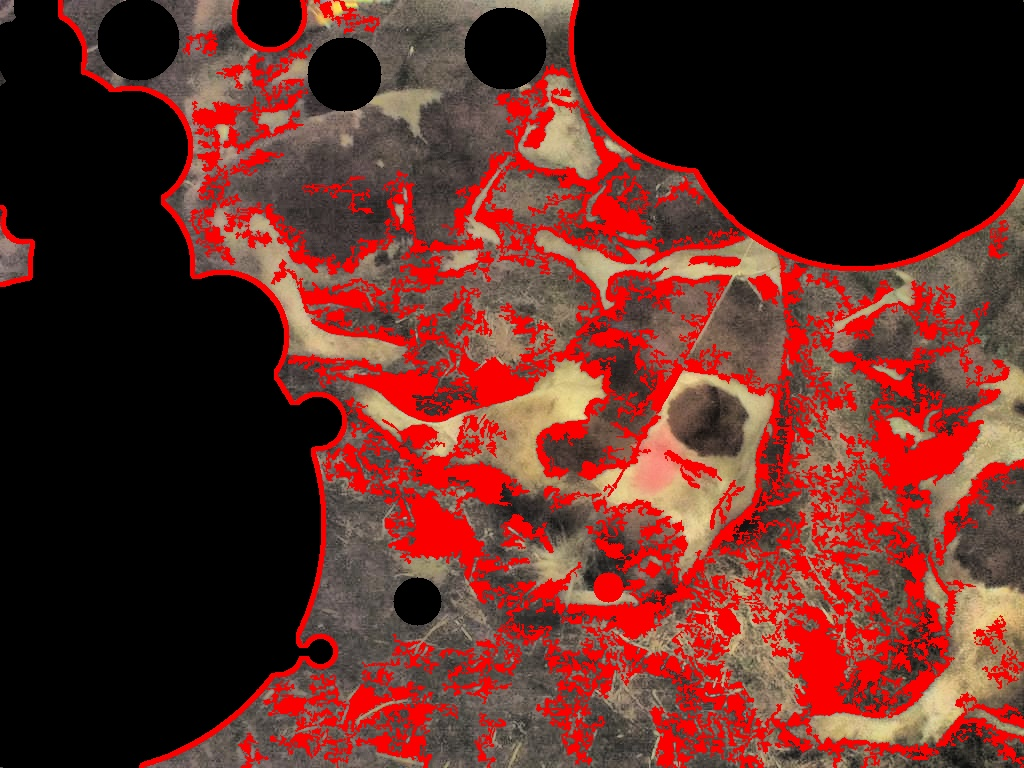
\includegraphics[scale=0.43]{Grafiken/entwicklung/10thresholdedEqualizedBirghtened.jpg}
	\caption{Detektierung von wichtigen Bereichen mittels adaptivem Schwellwertverfahren} 
	\label{fig: Detektierung von wichtigen Bereichen mittels adaptivem Schwellwertverfahren} 
\end{figure}

Das Ergebnis ist in Abbildung \ref{fig: Versuch, aus nicht geglättetem Bild wichtige Bereiche zu detektieren} dargestellt und stellt ein besseres Zwischenergebnis dar. Als entsprechende Erkenntnis leitet der Autor ab, dass die Glättung von Histogrammen zwar die Bildqualität und Interpretationsfähigkeit für den Menschen steigert, aber im vorliegenden Kontext auch negativen Einfluss auf das Schwellwertverfahren hat.

\begin{figure}[H]
	\center
	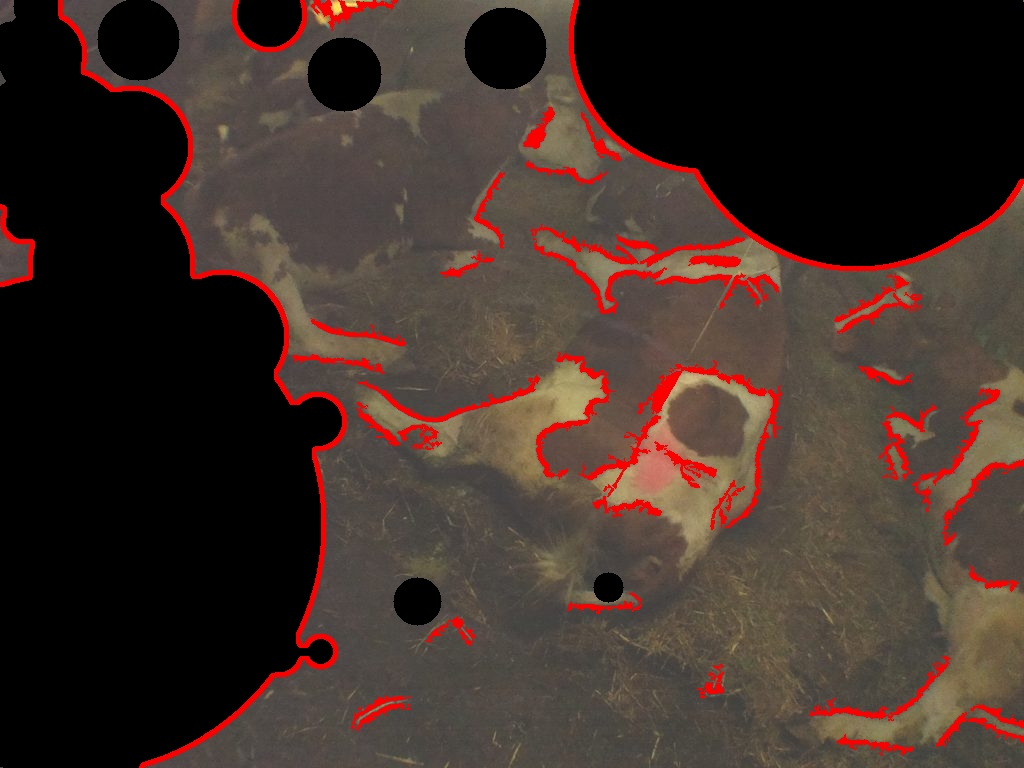
\includegraphics[scale=0.43]{Grafiken/entwicklung/11thresholdedNotEqualized.jpg}
	\caption{Versuch, aus nicht geglättetem Bild wichtige Bereiche zu detektieren} 
	\label{fig: Versuch, aus nicht geglättetem Bild wichtige Bereiche zu detektieren} 
\end{figure}

Abbildung \ref{fig: Versuch, aus nicht geglättetem Bild wichtige Bereiche zu detektieren} zeigt das Resultat einer vielversprechenden Analyse. Das Ergebnis ist aber insofern kritisch zu beurteilen, da die rote Farbe die gesamte Kontur ausfüllt, die detektiert wurde. Dementsprechend werden die Beine beispielsweise nicht als Kontur erkannt, sondern lediglich die Umrisse davon.
Dies dient als Motivation, die Konfiguration des Schwellwertverfahren anzupassen. Demzufolge wurde mit der Funktion \texttt{threshold()} und den Argumenten \texttt{THRESH_BINARY} als Verfahrenstyp, und dem Wert \texttt{90} als Schwellwert angewendet. Das Ergebnis daraus ist in Abbildung \ref{fig: Ergebnisse nach angepasster Konfiguration des Schwellwertverfahrens} dargestellt. Die als unwichtig identifizierten Bereiche werden nicht mehr berücksichtigt.
\begin{figure}[H]
	\center
	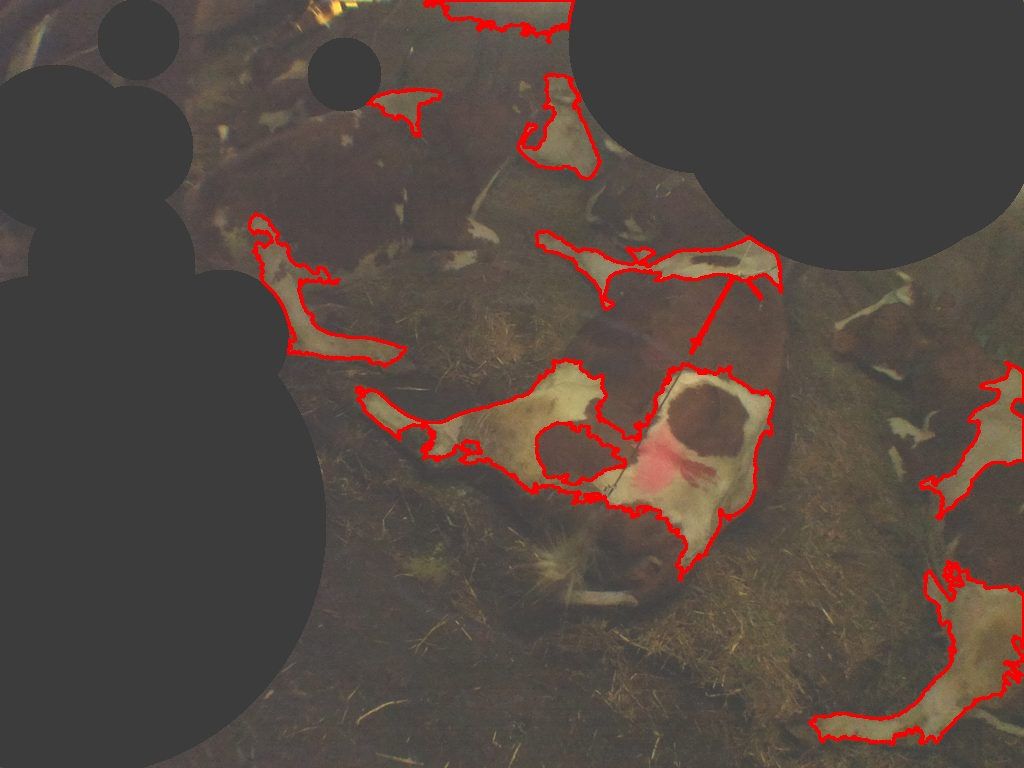
\includegraphics[scale=0.43]{Grafiken/entwicklung/12SimpleThresholdingConoturOutlineCCOMP.jpg}
	\caption{Ergebnisse nach angepasster Konfiguration des Schwellwertverfahrens} 
	\label{fig: Ergebnisse nach angepasster Konfiguration des Schwellwertverfahrens} 
\end{figure}
Es fällt nun auf, dass Flecken innerhalb der Kontur der Kuh erkannt werden. Da \texttt{findContours()} mit dem Argument \texttt{RETR_CCOMP} aufgerufen wird, werden auch Konturen innerhalb von den äusseren Konturen zurückgegeben und in eine  Hierarchie eingeteilt. Die äusseren Konturen entsprechen in den meisten Fällen den Umrissen der Kuh oder der Flecken. Zum aktuellen Zeitpunkt reicht es aus, nur diese Umrisse zu erkennen und dementsprechend wird \texttt{findContours()} mit dem Argument \texttt{RETR_EXTERNAL} aufgerufen. Das Ergebnis ist in Abbildung  \ref{fig: Ergebnisse nach angepasster Konfiguration des Contour Finders} sichtbar.
\begin{figure}[H]
	\center
	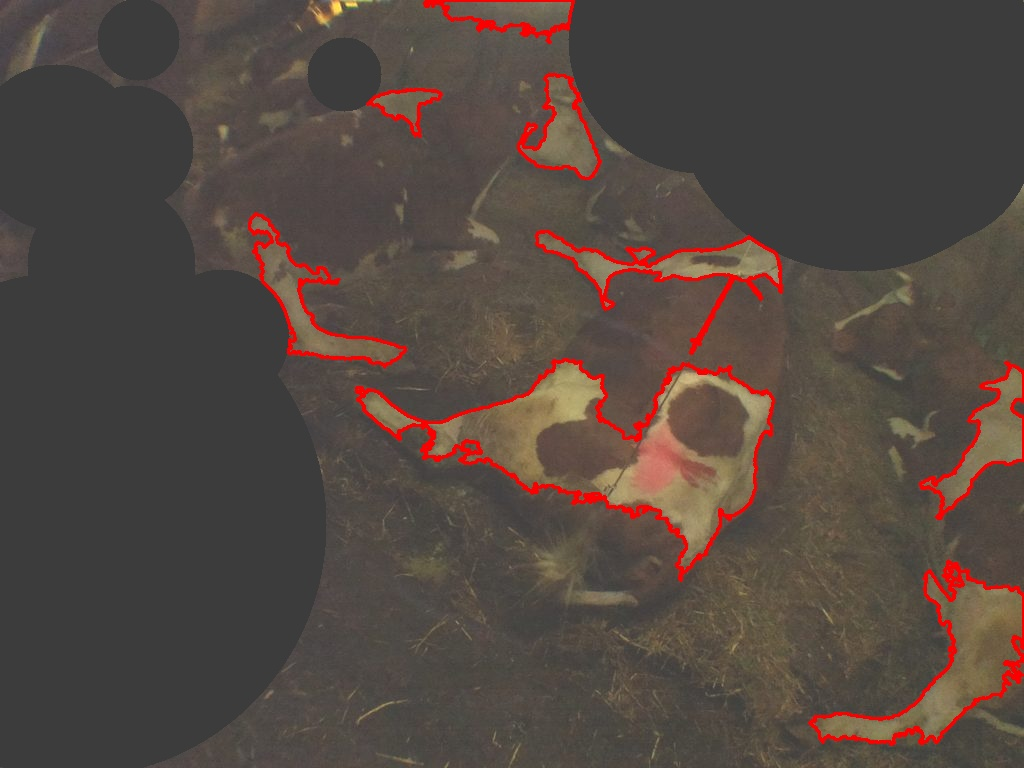
\includegraphics[scale=0.43]{Grafiken/entwicklung/13SimpleThresholdingConoturOutlineLIST.jpg}
	\caption{Ergebnisse nach angepasster Konfiguration des Contour Finders} 
	\label{fig: Ergebnisse nach angepasster Konfiguration des Contour Finders} 
\end{figure}

Dabei unterscheiden sich die Ergebnisse bei der Anwendung von \texttt{findContours()} mit unterschiedlichen Approximationsverfahren wie \texttt{CHAIN_APPROX_SIMPLE}, \texttt{CHAIN_APPROX_TC89_L1}, \texttt{CHAIN_APPROX_TC89_KCOS} von der Deaktivierung der Approximation  nicht wesentlich.

Da nun lediglich äussere Konturen detektiert werden, dürfen diese Konturen mit Farbe gefüllt werden, ohne relevante Informationen über Hierarchien zu vernichten (Abbildung \ref{fig: Konturen mit Farbe gefüllt}).

\begin{figure}[H]
	\center
	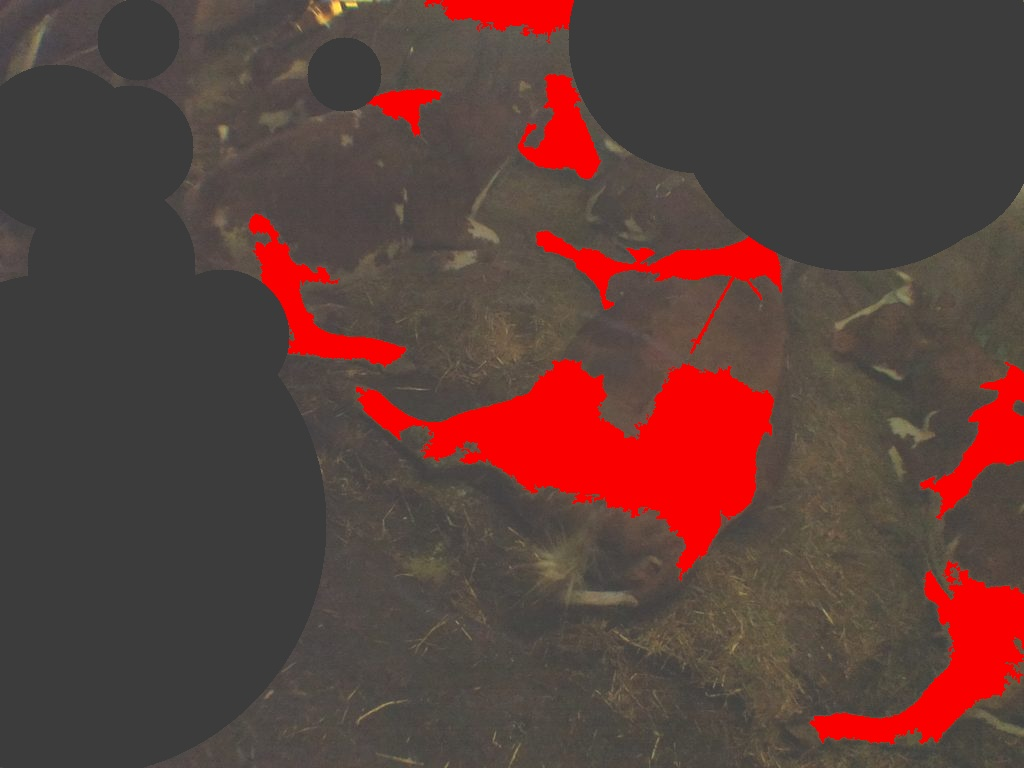
\includegraphics[scale=0.43]{Grafiken/entwicklung/14AfterThresholdingContourFilled.jpg}
	\caption{Konturen mit Farbe gefüllt} 
	\label{fig: Konturen mit Farbe gefüllt} 
\end{figure}


\subsection{Erkennung von seitlich liegender Kuh}
Aus der Domänenanalyse und Experteninterviews hat sicher ergeben, dass seitliches Liegen ein starkes Geburtsanzeichen ist und entsprechend detektiert werden muss. Die Seitenlage charakterisiert sich unter anderem mit gestreckten Beinen. Um diese zu erkennen, werden die geometrischen Eigenschaften der detektierten Konturen nachfolgend mit unterschiedlichen Verfahren analysiert. Diese Analyse soll die Filterung der unwichtigen Konturen erlauben. 

 Da nun keine weiteren Konturen mehr gesucht werden (kein Aufruf von \texttt{findContours()}), sind nachfolgend sämtliche dargestellten Bilder bearbeitet, um deren Helligkeit und Kontrast zu erhöhen. Dies wurde unter Anwendung der Funktionen \texttt{add()} und \texttt{createCLAHE()} gemacht. Zudem wurden die schwarze Kreise, welche unwichtige Bereiche des Bildes verdecken entfernt. Dies erhöht die Lesbarkeit des Berichts. Zudem wurden Rechtecke gezeichnet, welche die Konturen jeweils umschliessen. Diese Erhöhen das Verständnis von den geometrischen Eigenschaften und Filterungen. Dabei werden Konturen rot eingefärbt, die als Resultat der Analyse als wichtig befunden werden. Diese werden schrittweise gefiltert. Konturen, welche in einem Zwischenschritt als unwichtig erkannt werden, werden mit grüner Farbe gefüllt. 

\begin{figure}[H]
	\center
	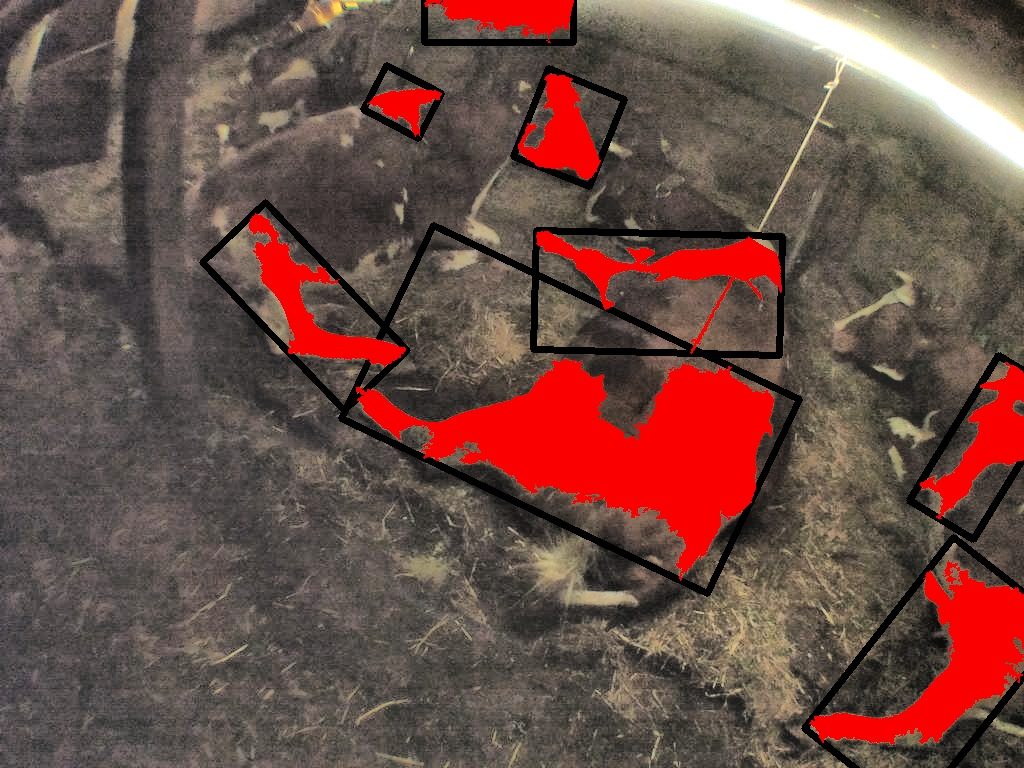
\includegraphics[scale=.43]{Grafiken/entwicklung/20StartImage.jpg}
	\caption{Ausgangslage vor der Analyse und Filterung der Konturen} 
	\label{fig: Ausgangslage vor der Analyse und Filterung der Konturen} 
\end{figure}

\subsubsection{Filterung der Konturen nach Winkel}
Typischerweise strecken Kühe in Seitenlage die Beine ungefähr rechtwinklig vom Körper weg. Die Infrastruktur vom Bauernhof des Arbeitgebers im Schwellibach ist auf Anbindehaltung ausgelegt. Wenn der Stall voll ist, also in jeder Box eine Kuh ist, liegen die Kühe beim Kalbern gerade in der Box \citep{Muller2020b}. Dementsprechend können Konturen als unwichtig betrachtet werden, wenn deren Ausrichtung stark von 90$^{\circ}$  abweicht. Als Referenzobjekt für die Messung des Winkels dient die Lampe, welche in Realität rechtwinklig zur Box der Kuh und waagrecht montiert ist. Da die Lampe in Bildern nicht waagrecht abgebildet ist, werden die Winkel sämtlicher Konturen um diese Abweichung bereinigt (Formel \ref{Bereinigung der Winkel}). Für die Messung der Winkel wurde die Funktion \texttt{fitEllipse()} verwendet, welche den Winkel der entsprechenden Ellipse zurückgibt.

\begin{equation}\label{Bereinigung der Winkel}
\delta_{i} = (\alpha_{i} - \beta + \gamma) \bmod 360
\end{equation}

wobei $ \delta_{i} $ dem bereinigten Winkel von Kontur ${i}$,  $ \alpha_{i} $ dem gemessenen Winkel von Kontur ${i}$, $\beta$ dem tatsächlichen Winkel der Lampe und $\gamma$ dem erwarteten Winkel der Lampe entspricht.


Das Vorgehen gleicht grundsätzlich dem Prinzip, das Bild solange zu drehen, bis die Lampe waagrecht im Bild ist und erst dann die Winkel zu messen. Abbildung \ref{fig: Veranschaulichung zur Analyse der Winkel} veranschaulicht die Überlegung. 


\begin{figure}[H]
	\center
	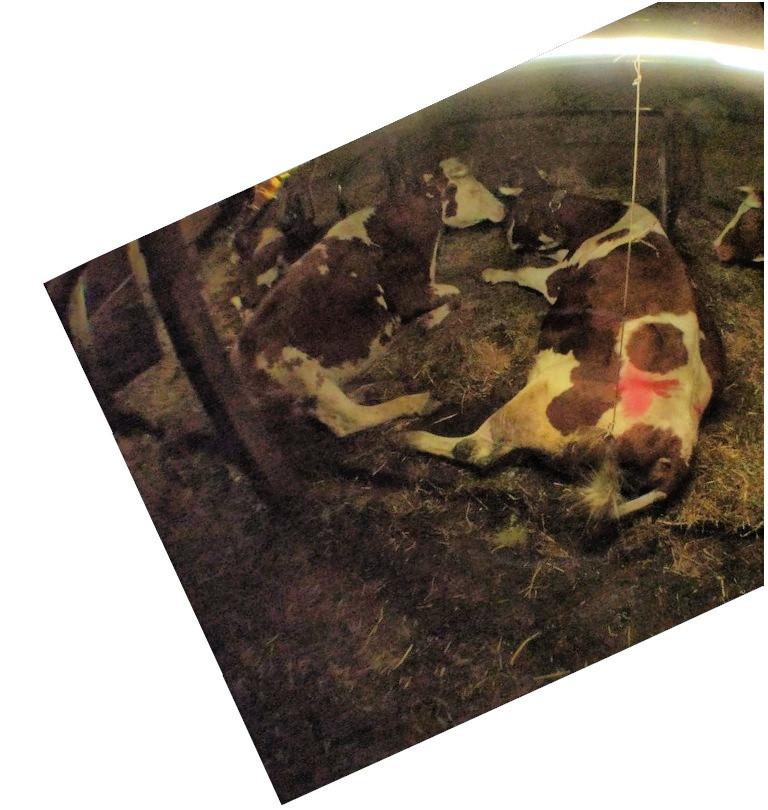
\includegraphics[scale=1.3]{Grafiken/entwicklung/21AngleCorrecturDemonstration.jpg}
	\caption{Veranschaulichung zur Analyse der Winkel} 
	\label{fig: Veranschaulichung zur Analyse der Winkel} 
\end{figure}


Die Abbildung \ref{fig: Ergebnisse nach Filterung der Konturen nach Winkel} zeigt in roter Farbe die Konturen, welche weiterhin als Beine von seitlich liegenden Kühen vermutet werden und entsprechend weiter analysiert werden. Die bereinigten Winkel der grün eingefärbten Konturen liegen nicht im Wertebereich zwischen \texttt{70-}\texttt{110}$^{\circ}$. Dabei sind die maximalen und minimalen Werte der betrachteten Winkel in der entwickelten Lösung mittels \texttt{MIN_LEG_ANGLE_EXPECTION} und \texttt{MAX_LEG_ANGLE_EXPECTION} konfigurierbar. 
\begin{figure}[H]
	\center
	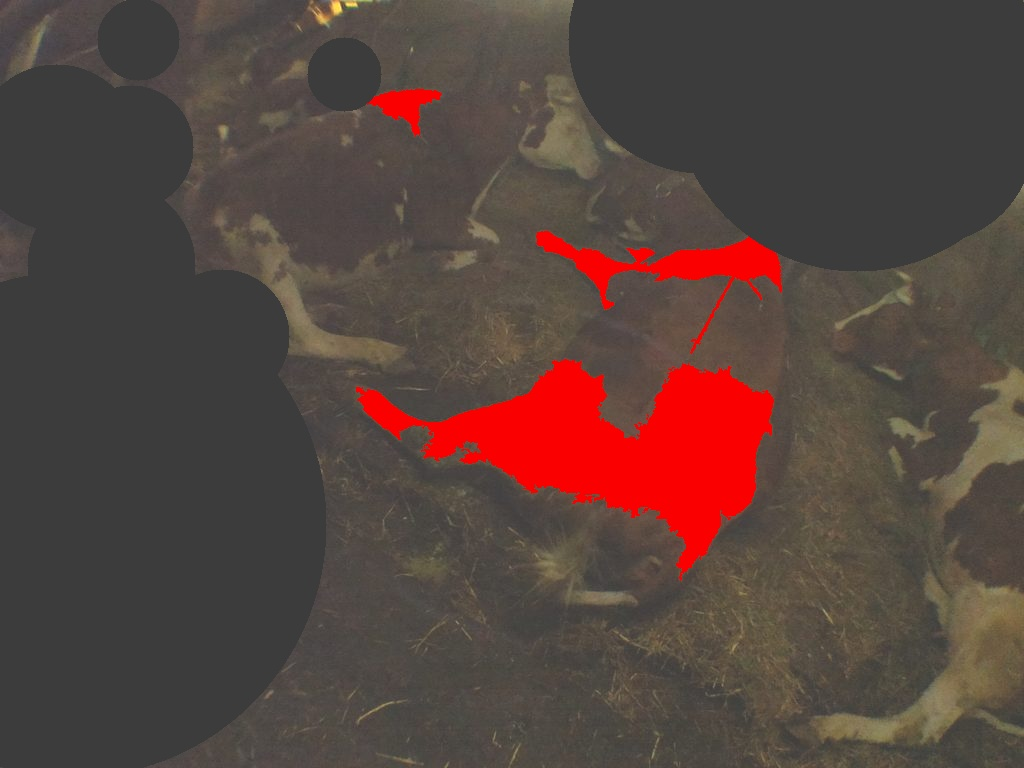
\includegraphics[scale=0.43]{Grafiken/entwicklung/22AngleCorrectur.jpg}
	\caption{Ergebnisse nach Filterung der Konturen nach Winkel} 
	\label{fig: Ergebnisse nach Filterung der Konturen nach Winkel} 
\end{figure}

Eine Ausnahme stellt ein nicht voller Stall dar. Leere Boxen ermöglichen der kalbernden Kuh, quer in die Box zu liegen \citep{Muller2020b}. Für Kühe, welche neben einer leeren Box liegen, ist also die Filterung der Konturen nach Winkel nicht sinnvoll. Um dieser Situation gerecht zu werden, kann im entwickelten System mittels Konfiguration \texttt{filterbyAngle=False} die Filterung nach Winkel deaktiviert werden. 


\subsubsection{Filterung der Konturen nach Extent}
Um diese Ergebnisse weiter zu analysieren, wurde mittels \texttt{minAreaRect()} für jede Kontur das Rechteck ermittelt, welches mit der kleinsten Fläche sämtliche Punkte der Kontur einschliesst. Die Rechtecke wurden schwarz ins Originalbild eingezeichnet. 
Dies dient als Grundlage des \flqq Extent\frqq. Dabei handelt es sich um das Verhältnis zwischen der Fläche der Kontur und der Fläche des Rechtecks, das die Kontur einschliesst (Formel \ref{Extent}).

\begin{equation}\label{Extent}
Extent =  \frac{Fl\ddot{a}che\ der\ Kontur}{Fl\ddot{a}che\  umschliessendes\  Rechteck}  
\end{equation}

Der Autor erwartet, dass die Fläche der Kontur der Beine gegenüber dem darum gebildeten Rechteck klein ist. Entsprechend wird für als Extent bei Beinen ein tiefer Wert angenommen im Vergleich zum Wert des Extent bei anderen Figuren. Dementsprechend ermöglicht die entwickelte Lösung die Konstante \texttt{EXTENT_MAX} die Konfiguration eines Schwellwerts, nach welchem Konturen gefiltert werden. 

Nun wird als Schwellwert für Extent \texttt{0.5} angenommen und entsprechend werden nur noch Konturen berücksichtigt, welche unterhalb dieses Werts liegen. In Abbildung \ref{fig: Ergebnis der Filterung der Konturen nach Extent} sind alle Konturen mit ${Extent < 0.5}$ rot und alle anderen Konturen grün eingefärbt. Das Ergebnis ist positiv, zwei unerwünschte Konturen können als solche erkannt werden.
\begin{figure}[H]
	\center
	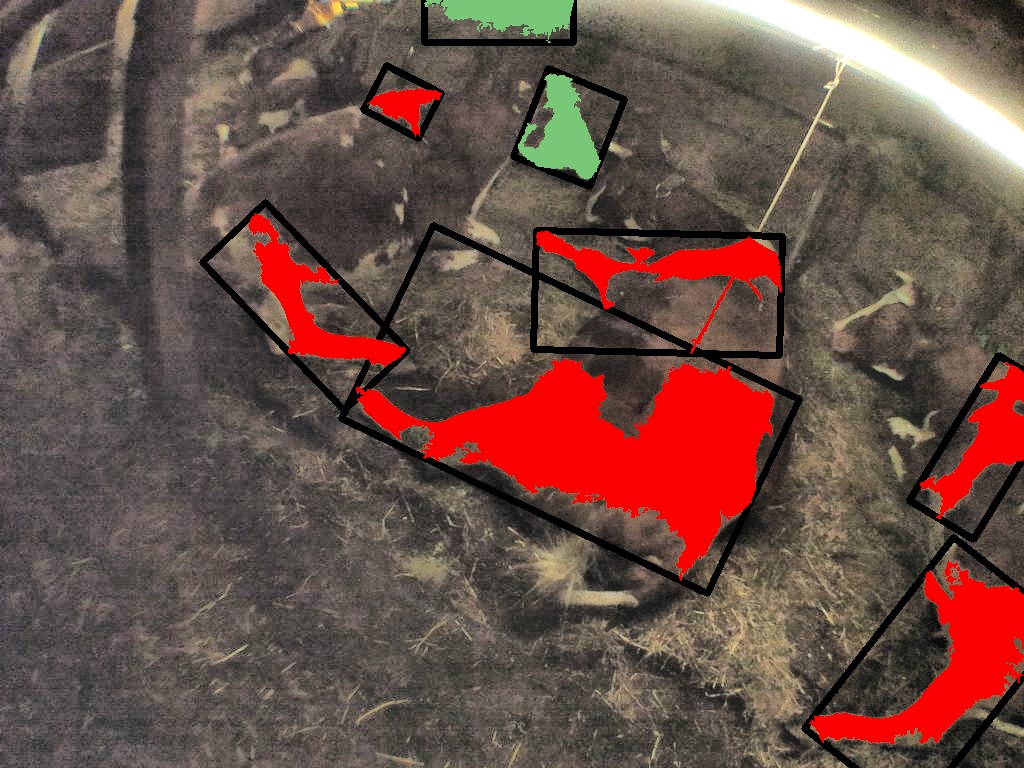
\includegraphics[scale=0.43]{Grafiken/entwicklung/23FilteringExtent.jpg}
	\caption{Ergebnis der Filterung der Konturen nach Extent } 
	\label{fig: Ergebnis der Filterung der Konturen nach Extent} 
\end{figure}

Abbildung \ref{fig: Ergebnis der Filterung der Konturen nach Winkel und Extent } veranschaulicht die Kombination der Filterung nach Winkel und Extent. Es können erfolgreich unwichtige Konturen gefiltert werden. Um die Ergebnisse der Analyse zu verbessern, sind jedoch zusätzlich Filterungen nötig.
\begin{figure}[H]
	\center
	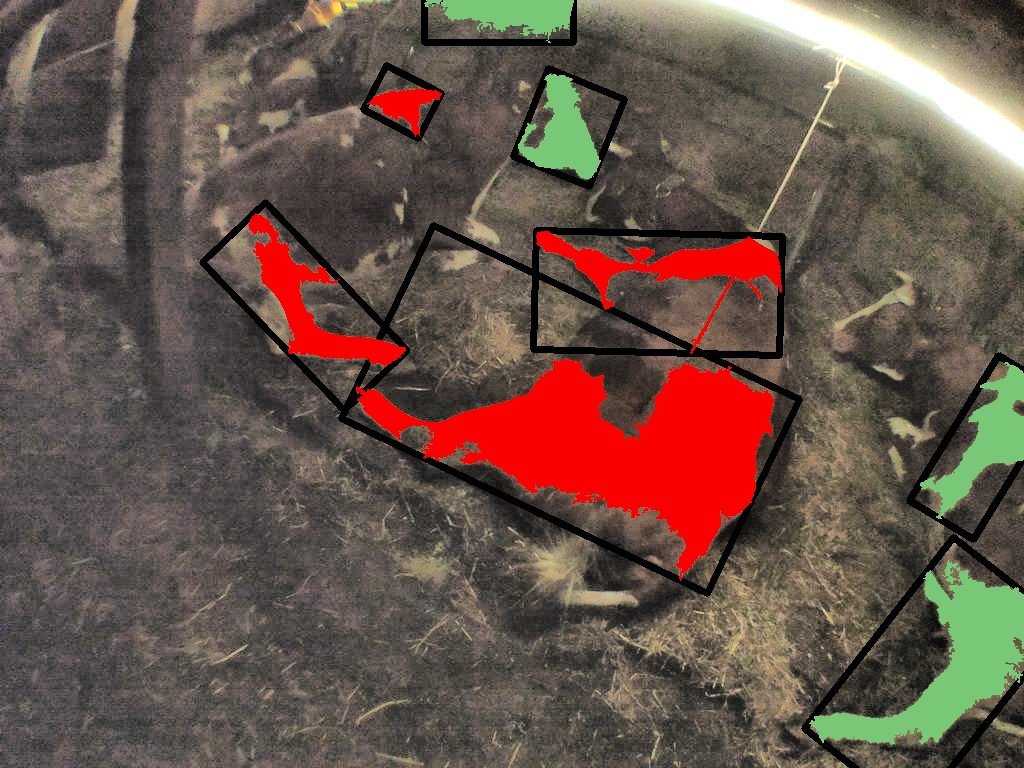
\includegraphics[scale=0.43]{Grafiken/entwicklung/24FilteringExtentAngle.jpg}
	\caption{Ergebnis der Filterung der Konturen nach Winkel und Extent  } 
	\label{fig: Ergebnis der Filterung der Konturen nach Winkel und Extent } 
\end{figure}

\subsubsection{Filterung der Konturen nach Aspect Ratio}

Rechtecke, welche die Beine der Kuh einschliessen, sind langgezogen. Der Autor überprüft nun die Vermutung, dass diese Eigenschaft dabei hilf, Beine von unwichtigen Konturen zu unterscheiden. Das Verhältnis zwischen Breite und Höhe von Rechtecken (nachfolgend Aspect Ratio genannt) liefert Informationen darüber, wie langgezogen ein Rechteck ist.	
	
\begin{equation}\label{Aspect Ratio}
Aspect\ Ratio =  \frac{Breite}{H\ddot{}he}  
\end{equation}
Da für den Autor grundsätzlich nicht das Verhältnis zwischen Breite und Höhe sondern das Verhältnis zwischen der langen und der kurzen Seite des Rechtecks entscheidend ist, wird die Formel \ref{Aspect Ratio} angepasst. Formel \ref{Angepasste Aspect Ratio} beschreibt, was in der technischen Implementierung realisiert wird.
\begin{equation}\label{Angepasste Aspect Ratio}
Aspect\ Ratio =  \frac{lange \ Seite}{kurze \ Seite}  
\end{equation}

Das Ergebnis der Filterung von Konturen mit dem Schwellwert \texttt{1.5} ist in Abbildung \ref{fig: Ergebnis der Filterung von Konturen nach Aspect Ratio} abgebildet. Die Filterung der Konturen kann dadurch verbessert werden.
\begin{figure}[H]
	\center
	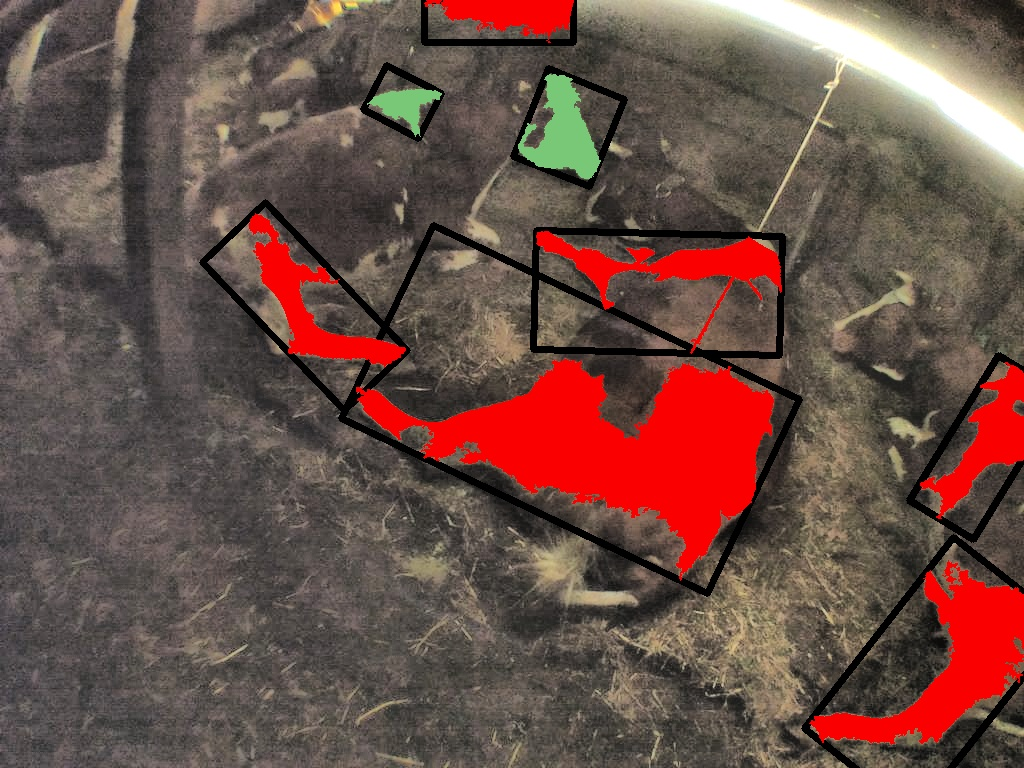
\includegraphics[scale=0.43]{Grafiken/entwicklung/27AspectRatio.jpg}
	\caption{Ergebnis der Filterung von Konturen nach Aspect Ratio } 
	\label{fig: Ergebnis der Filterung von Konturen nach Aspect Ratio} 
\end{figure}
\subsubsection{Kombination der Filter nach Winkel, Extent und Aspect Ratio }
Durch Kombination der Filterung nach Winkel, Extent und Aspect Ratio, erreicht man das Resultat gemäss Abbildung \ref{fig: Ergebnis der Filterung der Konturen nach Winkel, Extent und Aspect Ratio}. Dabei werden Konturen mit einem bereinigten Winkel zwischen \texttt{70} und \texttt{110}$^{\circ}$, Extent unter 0.5 und Aspect Ratio über 1.5 berücksichtigt.



\begin{figure}[H]
	\center
	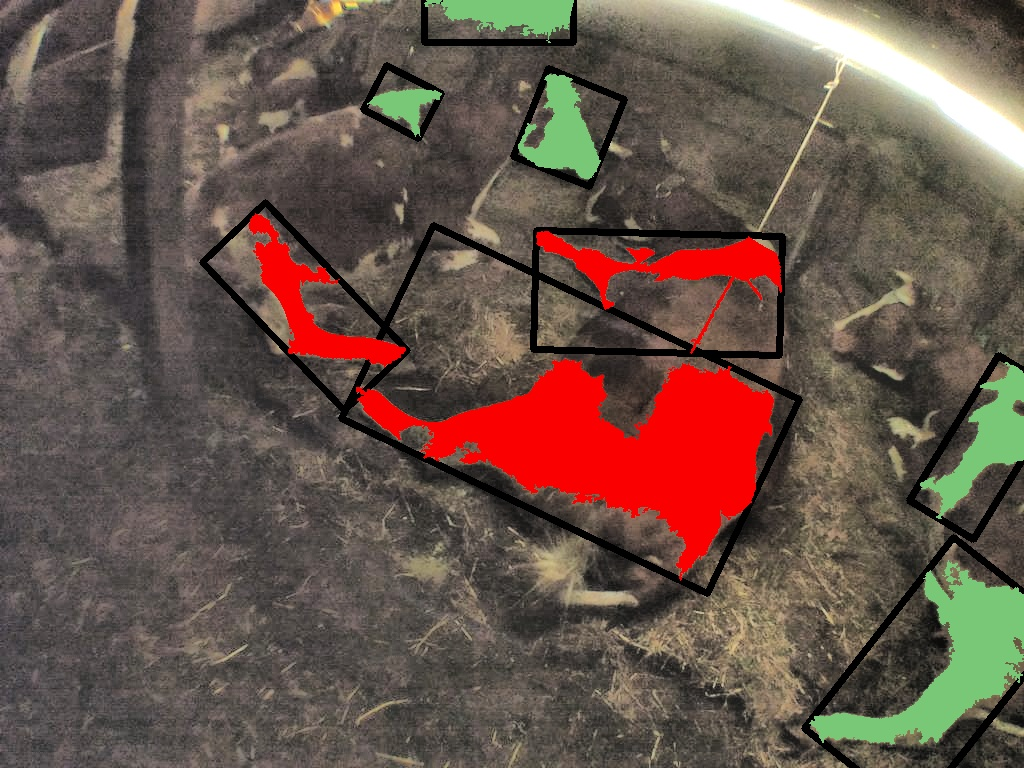
\includegraphics[scale=0.43]{Grafiken/entwicklung/30FilteredByExtentAspectAngle.jpg}
	\caption{Ergebnis der Filterung der Konturen nach Winkel, Extent und Aspect Ratio} 
	\label{fig: Ergebnis der Filterung der Konturen nach Winkel, Extent und Aspect Ratio} 
\end{figure}

\subsubsection{Filterung mittels Shape Matching }
Nun werden vier Konturen als potentielle Konturen von Beinen bei seitlichem Liegen erkannt. Wünschenswert wäre nun, diese Auswahl weiter einzugrenzen. Um dies zu erreichen, sind Unterschiede der Konturen von den Beinen der mittleren Kuh und der Kontur des Hinterbeins der linken Kuh zu ermitteln. In erster Linie hat der Autor versucht, die Orientierung der Beine zu erkennen. Beim seitlichen Liegen der Kuh zeigen zwei Beine in dieselbe Richtung und deren Abstand liegt innerhalb eines bestimmten Bereichs. Anhand der Ausrichtung der Beine kann mit den bereits angewendeten Funktionen \texttt{minAreaRect()} und \texttt{fitEllipse()} keine weitere Filterung etabliert werden. Der Grund dafür ist, dass sämtliche Winkel in einem sehr ähnlichen Wertebereich sind. Auch die Messung des Abstands zwischen den Beinen ist mit den bereits angewendeten Mitteln nicht möglich. Der Autor ist der Meinung, dass sich im betrachteten Bild in erster Linie der Holzträger als Referenzobjekt für die Messung von Distanzen eignet. Dieser ist jedoch nicht in voller Länge im Bild, was die Messung ungenau macht. Darüber hinaus ist dieser Holzträger nicht in jedem Bild an derselben Stelle und auch nicht in jedem Bild sichtbar. Die Konturen der Beine sind keine geeigneten Referenzobjekte, da diese gestreckt oder gebeugt sein können. Der Autor ist der Ansicht, dass ein Referenzobjekt im Bild platziert werden müsste, um gute Resultate zu erreichen. Dieses Referenzobjekt sollte durch Methoden der Bildanalyse eindeutig zu erkennen sein.

An dieser Stelle verfolgt der Autor einen anderen Lösungsansatz. Die Funktion \texttt{matchShapes()} vergleicht sämtliche verbleibende Konturen und gibt eine Metrik zurück, welche die Ähnlichkeit der Konturen repräsentiert. Die Funktion unterstützt die drei Modi \texttt{CONTOURS_MATCH_I1}, \texttt{CONTOURS_MATCH_I2} und \texttt{CONTOURS_MATCH_I3} \citep[S. 392]{FernandezVillan2019}. Sämtliche Modi ergeben im vorliegenden Kontext keinen Beitrag zur weiteren Filterung der Konturen. Bild \ref{fig: Ergebnis der Shape Matching} zeigt die Anwendung von \texttt{matchShapes()} mit dem Modus \texttt{CONTOURS_MATCH_I1} und dem Schwellwert \texttt{5}. Die Konturen der Hinterbeine der zwei Kühe werden als ähnlicher betrachtet als die Konturen der Beine derselben Kuh. 

\begin{figure}[H]
	\center
	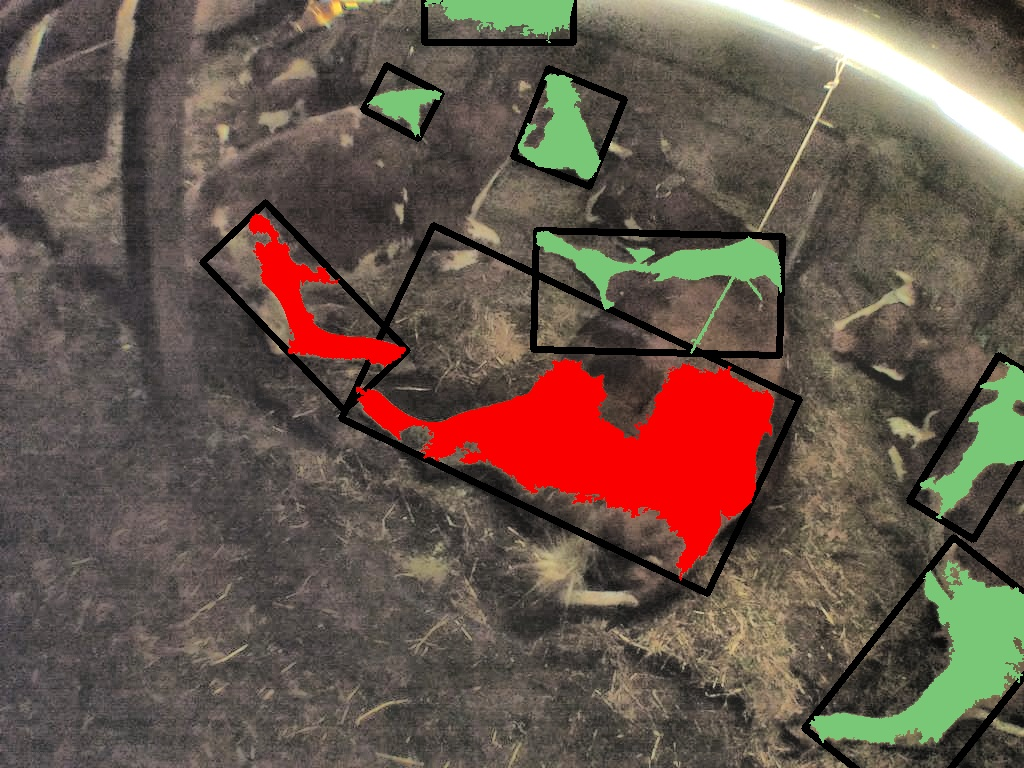
\includegraphics[scale=0.43]{Grafiken/entwicklung/31FilteredBySimilarity.jpg}
	\caption{Ergebnis der Shape Matching} 
	\label{fig: Ergebnis der Shape Matching} 
\end{figure}
Im angewandten Verfahren der Bildanalyse wurden die Winkel der Konturen bereits berücksichtigt. Um sicherzustellen, dass das Resultat von \texttt{matchShapes()} nicht auf die Winkel der Konturen zurückzuführen ist, werden sämtliche verbleibende Konturen auf einen zufällig ausgewählten Winkel von 60$^{\circ}$ verschoben. Anschliessend werden die Konturen wieder mit \texttt{matchShapes()} verglichen. Das Ergebnis ist dasselbe, die Klassifikation kann zu diesem Zeitpunkt nicht weiter verbessert werden. Abbildung \ref{fig: Ergebnis der Shape Matching und Korrektur der Winkel} zeigt die das Ergebnis der verschobenen Konturen mit einem weissen Hintergrund.
\begin{figure}[H]
	\center
	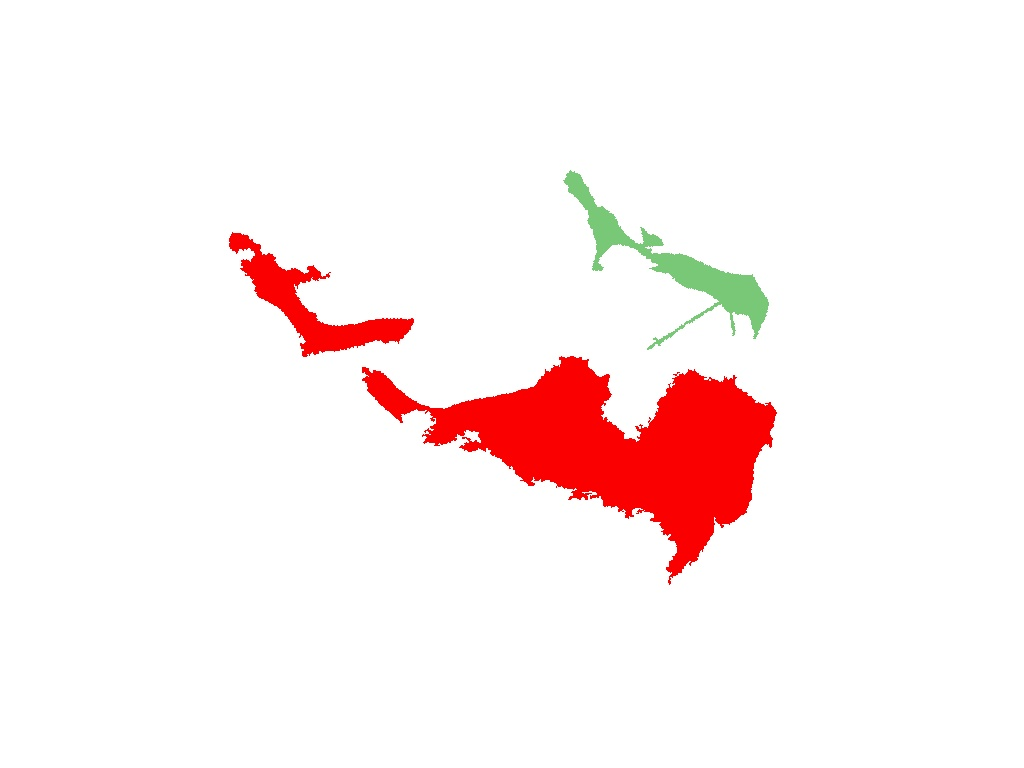
\includegraphics[scale=0.43]{Grafiken/entwicklung/32BlankFilteredBySimilarity.jpg}
	\caption{Ergebnis der Shape Matching und Korrektur der Winkel} 
	\label{fig: Ergebnis der Shape Matching und Korrektur der Winkel} 
\end{figure}


Die Abbildung \ref{fig: Ergebnis der Filterung der Konturen nach Winkel, Extent und Aspect Ratio} zeigt das beste Resultat. Sämtliche rot eingefärbten Konturen entsprechen dabei Konturen, welche korrekterweise seitwärts gestreckten Beinen entsprechen. Sowohl die Voder- als auch die Hinterbeine der betrachteten Kuh werden erkannt und entsprechend gekennzeichnet.

	% ================================================================
% CHAPTER 5: Resultate
% ================================================================


\chapter{Resultate}


Im Rahmen der vorliegenden Arbeit wurde eine Domänenanalyse zur automatischen Analyse von Kamerabildern bei der Geburt von Kälbern gemacht. Dabei wurde ein umfassendes System modelliert, welches sowohl die automatische Analyse von Kamerabildern als auch die Benachrichtigung der Stakeholder ermöglicht. Zudem erlaubt das modellierte System die Erfassung der medizinischen Daten von Kuh und Kalb. Dies ermöglicht dem Landwirten oder Tierarzt beispielsweise Zugriff auf die Krankheitsgeschichte oder den Verlauf der letzten Geburten einer Kuh. Dies unterstützt eine Beurteilung der Situation durch Fachpersonen. 

Dabei ist der Kern der Domänenanalyse die Identifikation von Geburtsmerkmalen. Im Wesentlichen hat sich ergeben, dass das System bei Erkennung von seitlichem Liegen und Anwesenheit der Wasser- oder Schleimblase eine Benachrichtigung an die Stakeholder auslösen muss. 

Der Kern des modellierten Systems wurde in Code umgesetzt. Es wurde ein flexibles und konfigurierbares System entwickelt, welches die automatische Analyse von Kamerabildern ermöglicht.

In den folgenden Abbildungen bedeuten grün eingefärbte Flächen, dass das System Konturen erkannt hat, diese aber nicht als Merkmal für eine Kuh in Seitenlage betrachtet. Rote Flächen bedeuten, dass das System diese Kontur als Merkmal für Seitenlage interpretiert.

In den Abbildungen \ref{fig: Korrektes Ergebnis von Analyse der stehenden Kuh} und \ref{fig: Weiteres korrektes Ergebnis von Analyse der stehenden Kuh} erkennt das System korrekterweise, dass keine Kuh in Seitenlage im Bild steht.

\begin{figure}[H]
	\center
	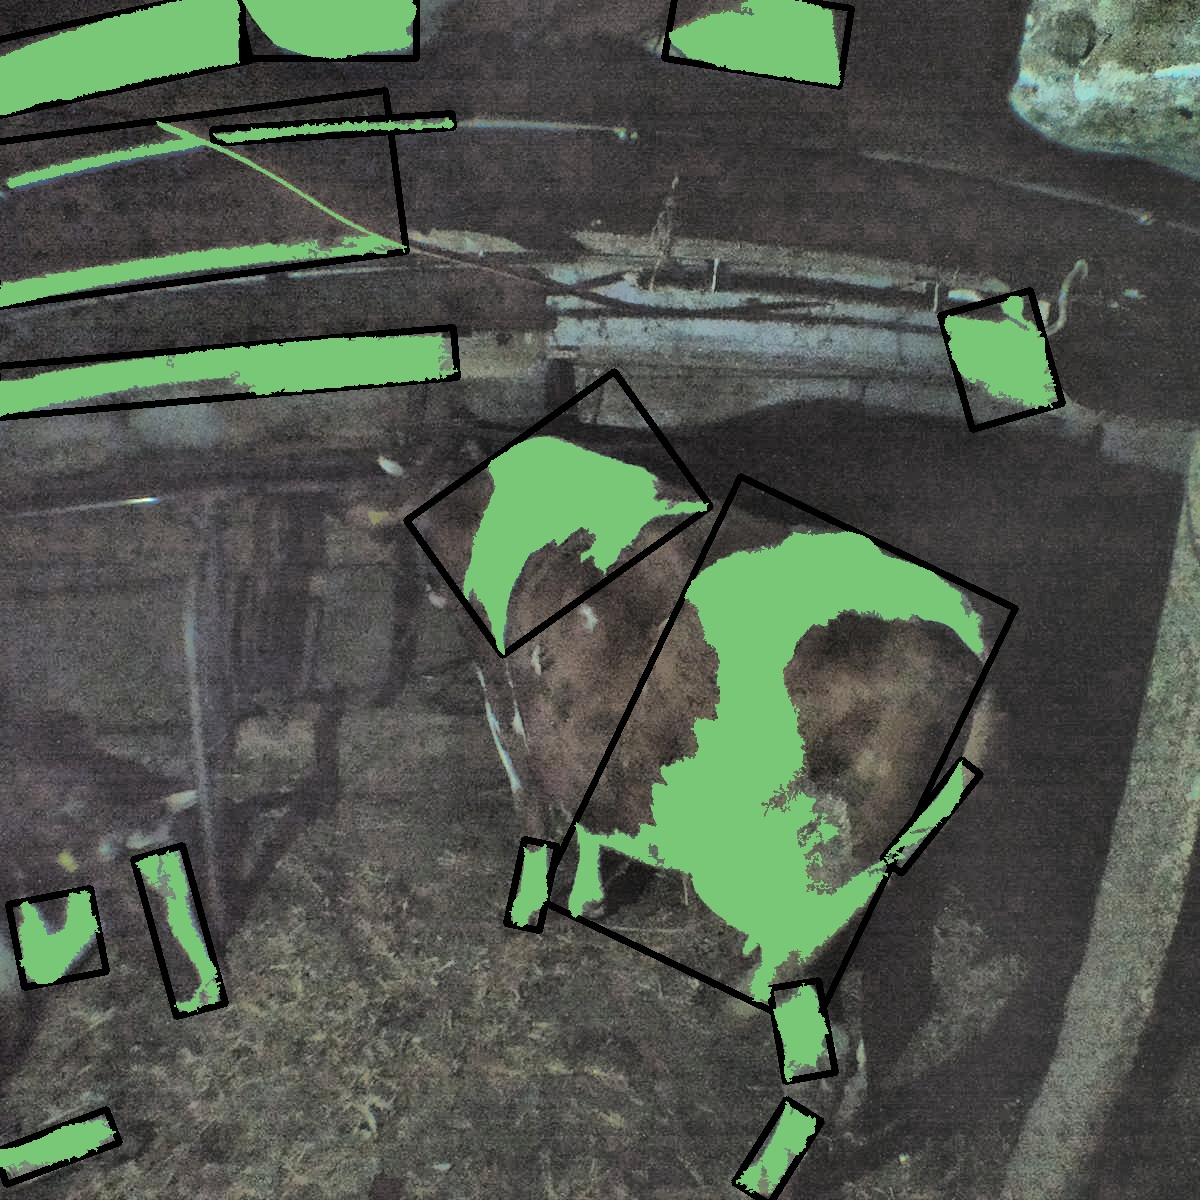
\includegraphics[scale=0.3]{Grafiken/resultate/resultatStanding2.jpg}
	\caption{Korrektes Ergebnis von Analyse der stehenden Kuh} 
	\label{fig: Korrektes Ergebnis von Analyse der stehenden Kuh} 
\end{figure}



\begin{figure}[H]
	\center
	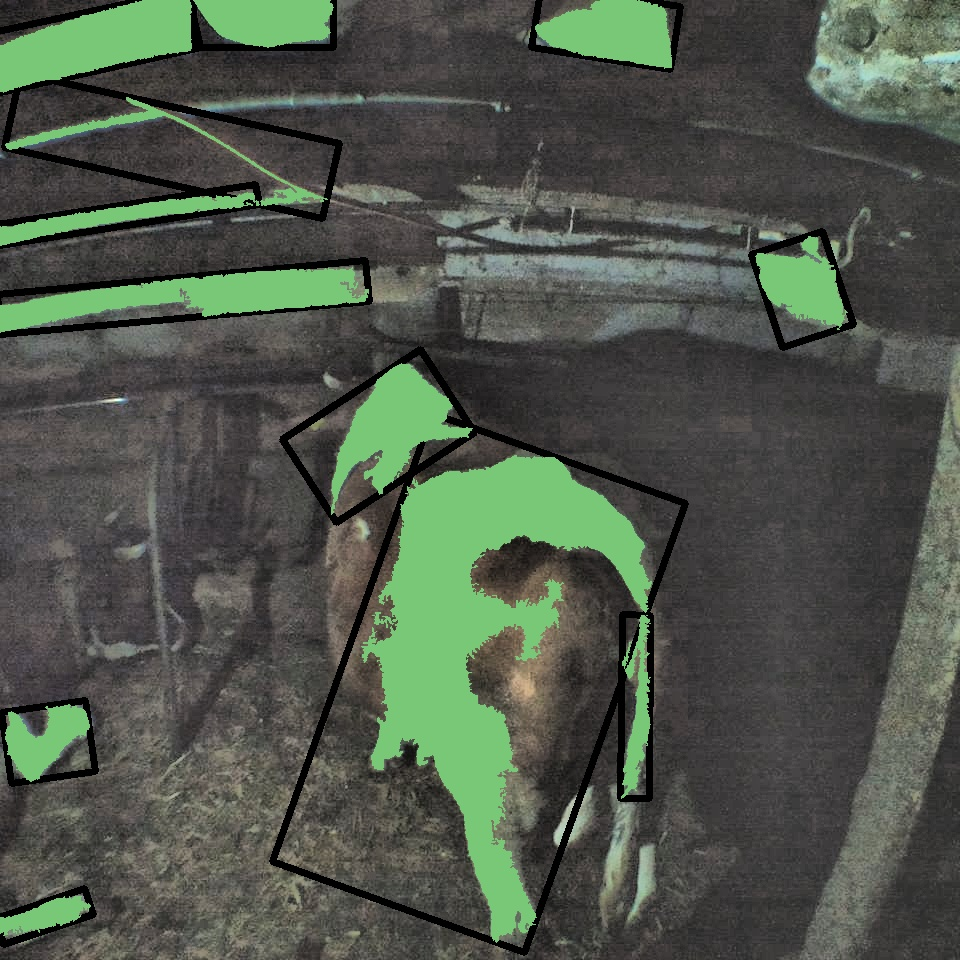
\includegraphics[scale=0.3]{Grafiken/resultate/resultatStanding1.jpg}
	\caption{Weiteres korrektes Ergebnis von Analyse der stehenden Kuh} 
	\label{fig: Weiteres korrektes Ergebnis von Analyse der stehenden Kuh} 
\end{figure}

In den Abbildungen \ref{fig: Korrektes Ergebnis von Analyse der Kuh in Seitenlage} und \ref{fig: Weiteres korrektes Ergebnis von Analyse der Kuh in Seitenlage} erkennt das System korrekterweise, dass sich die abgebildete Kuh in Seitenlage befindet. 

\begin{figure}[H]
	\center
	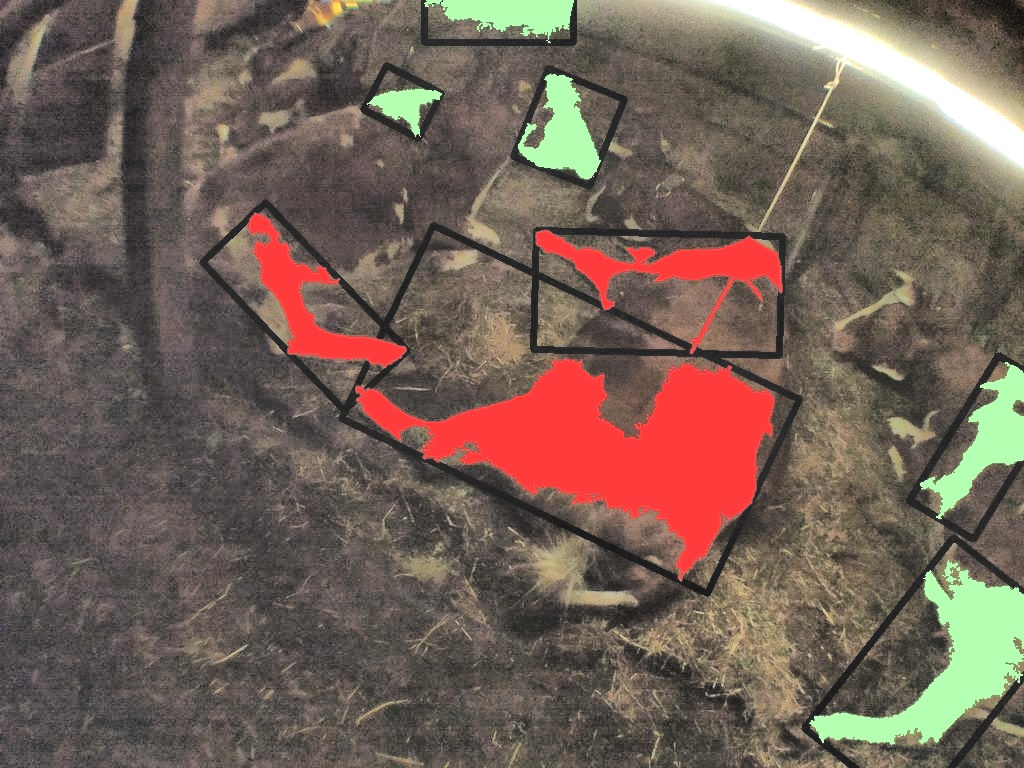
\includegraphics[scale=0.43]{Grafiken/resultate/resultatLying1.jpg}
	\caption{Korrektes Ergebnis von Analyse der Kuh in Seitenlage} 
	\label{fig: Korrektes Ergebnis von Analyse der Kuh in Seitenlage} 
\end{figure}


\begin{figure}[H]
	\center
	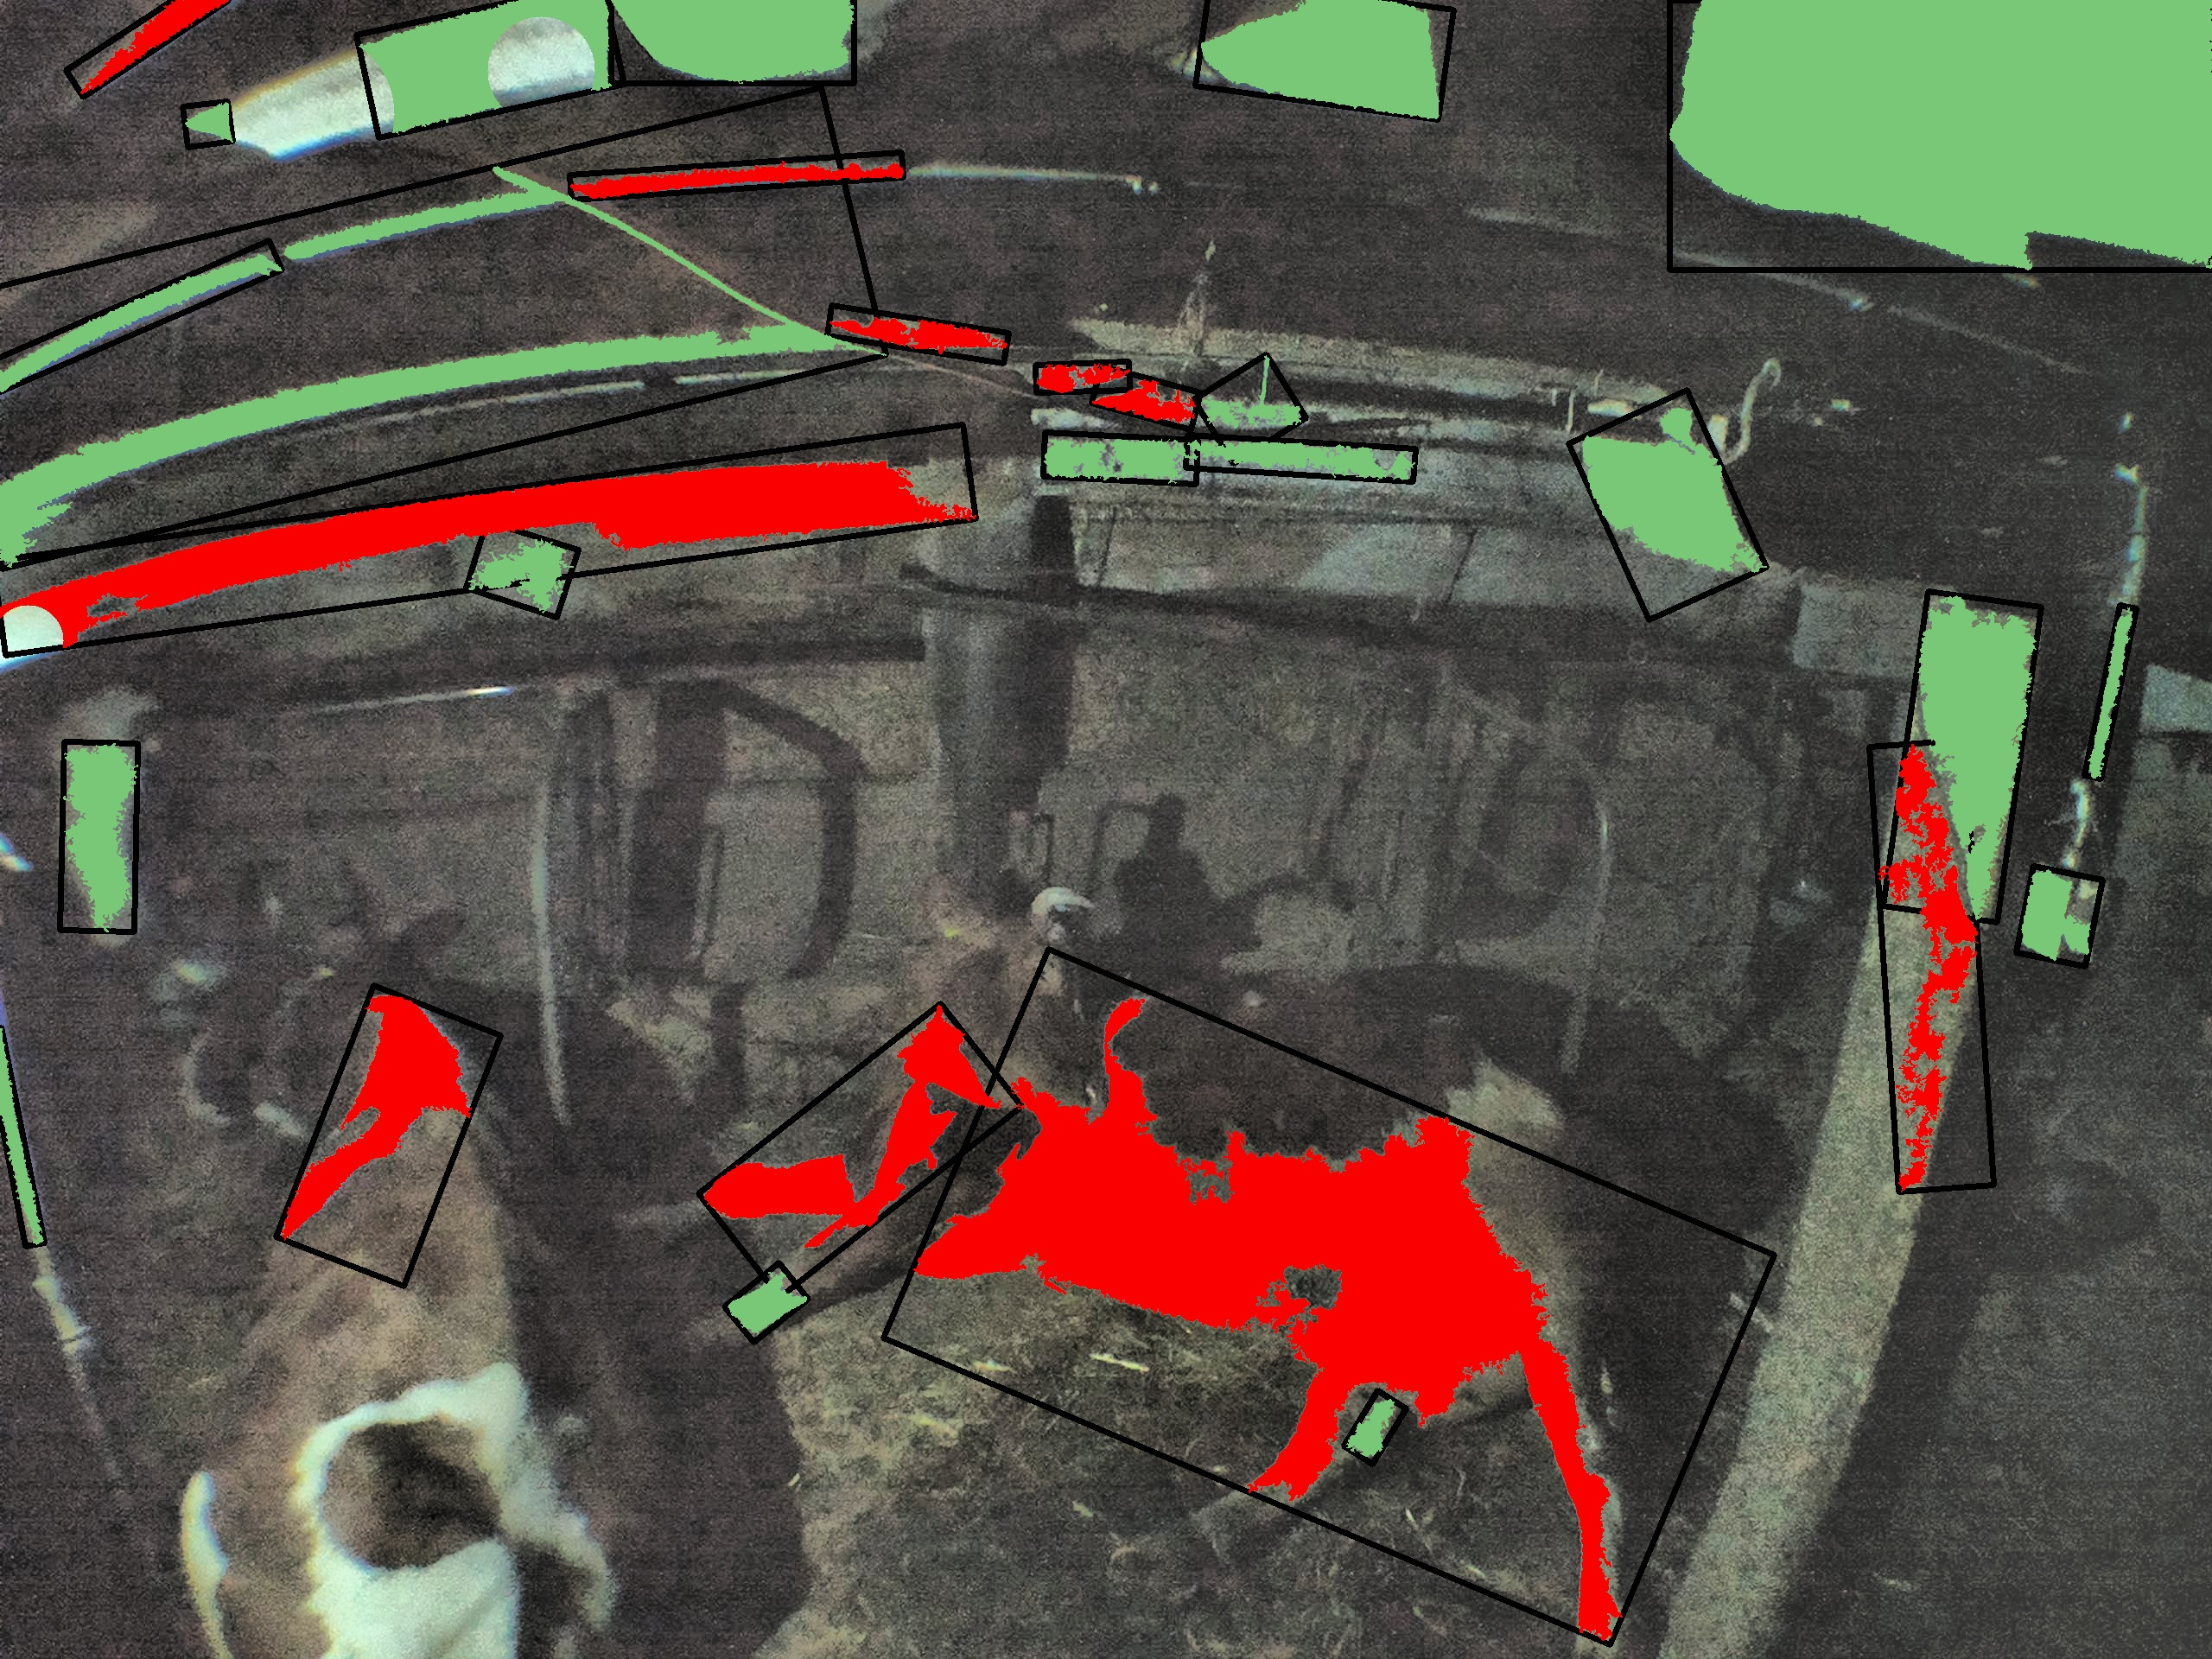
\includegraphics[scale=1.5]{Grafiken/resultate/resultatLying2.jpg}
	\caption{Weiteres korrektes Ergebnis von Analyse der Kuh in Seitenlage} 
	\label{fig: Weiteres korrektes Ergebnis von Analyse der Kuh in Seitenlage} 
\end{figure}

Um die bestmöglichen Ergebnisse zu erzielen, ist jedoch jeweils eine angepasste Konfiguration notwendig.
Einerseits muss jeweils eingestellt werden, ob nur die Farbwerte der Lampe als unwichtige Farbewerte zu interpretieren sind oder noch weitere Farben einen unwichtigen Bereich darstellen. Um zusätzliche Farbwerte als unwichtig zu deklarieren, kann diese Option mittels \texttt{ADVANCED_UNIMPORTANT_COLOR_RANGE=True} aktiviert werden. Anschliessend können beliebig viele Farbbereiche der Liste \texttt{additionalUnimportantColorRanges} hinzugefügt werden. Das System verarbeitet diese Liste an Farbbereichen und maximiert die als unwichtig identifizierbaren Bereiche.

Andererseits muss eingestellt werden, ob die Konturen nach Winkel gefiltert werden. Das System filtert die Konturen standardmässig nach Winkel, ermöglicht aber eine Deaktivierung dieser Funktionalität mittels \texttt{FILTER_BY_ANGLE=False}. Die fachliche Begründung dafür ist, dass nicht immer alle Boxen im Stall besetzt sind. Wenn eine Kuh neben einer leeren Box kalbert, kann sie sich quer über zwei Boxen legen. In dieser Situation ist eine Filterung der Konturen nach Winkel fachlich nicht sinnvoll.

Das System bietet zahlreiche weitere Konfigurationsmöglichkeiten. Die zwei genannten Optionen bilden fachlich  erheblichen Mehrwert. Experten können ohne Wissen über die technische Implementierung das System so konfigurieren, dass die Ergebnisse weiter verbessert werden. 

Als Beispiel dient das Ergebnis, welches in Abbildung \ref{fig: Fehlerhaftes Ergebnis von Analyse der Kuh in Seitenlage} sichtbar ist. Dieses Resultat wurde mit \texttt{FILTER_BY_ANGLE=False} und und \texttt{ADVANCED_UNIMPORTANT_COLOR_RANGE = False} erzielt. 
\begin{figure}[H]
	\center
	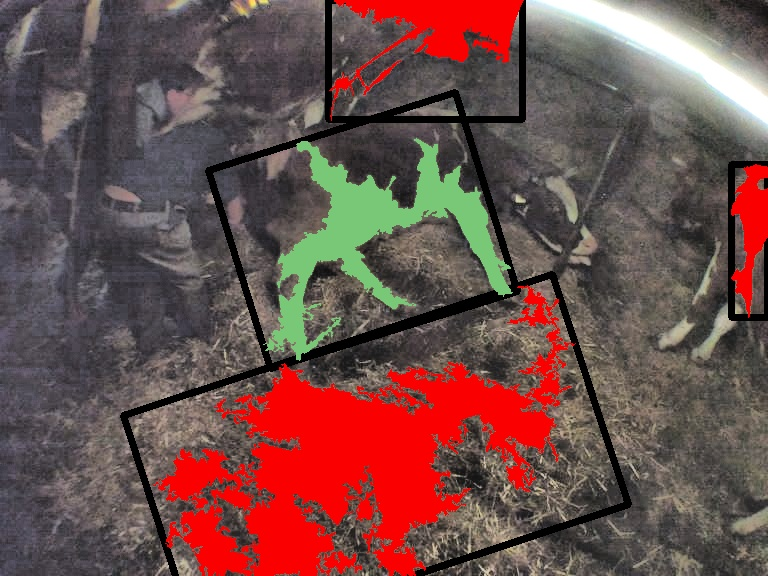
\includegraphics[scale=0.5]{Grafiken/resultate/resultatFehlerhaft.jpg}
	\caption{Fehlerhaftes Ergebnis von Analyse der Kuh in Seitenlage} 
	\label{fig: Fehlerhaftes Ergebnis von Analyse der Kuh in Seitenlage} 
\end{figure}

Durch die Konfiguration von \texttt{ADVANCED_UNIMPORTANT_COLOR_RANGE=True} und der Ergänzung zur Detektierung von unwichtigen Farbwerten im Bereich des Strohs und sehr hellen Bereichen im oberen Bildbereich kann das Ergebnis verbessert werden. In Abbildung \ref{fig: Verbessertes Ergebnis von Analyse der Kuh in Seitenlage} wird das Stroh nicht mehr fälschlicherweise als Kontur der Kuh interpretiert. Das Gesamtergebnis der Analyse ist trotzdem falsch, die Seitenlage wird nicht erkannt, weil das umschliessende Rechteck den Schwellwert für die minimale Aspect Ratio nicht erreicht. Dennoch veranschaulicht dieses Beispiel den erheblichen Mehrwert des konfigurierbaren Systems.

\begin{figure}[H]
	\center
	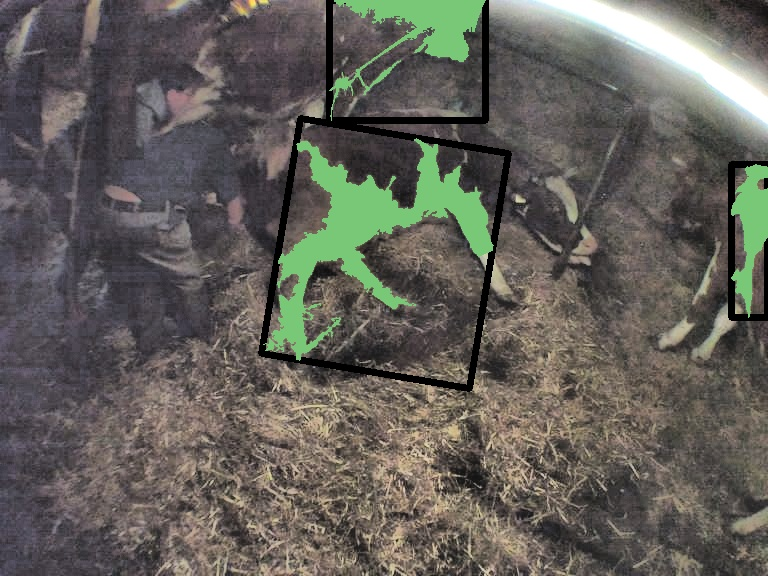
\includegraphics[scale=0.5]{Grafiken/resultate/verbessertesResultat.jpg}
	\caption{Verbessertes Ergebnis von Analyse der Kuh in Seitenlage} 
	\label{fig: Verbessertes Ergebnis von Analyse der Kuh in Seitenlage} 
\end{figure}


Die im Rahmen der Bachelor-Arbeit erarbeiteten Lieferergebnisse werden per E-Mail an Prof. Dr. Patrizio Collovà und Dr. Klaus-Georg Deck geschickt. Dies umfasst nebst dem Bericht ein Archiv mit dem Quellcode des entwickelten Systems, den erstellen Modellen und dem Code zur Analyse der Daten aus den Interviews. 

Zudem ist der gesamte Quellcode des entwickelten Systems auf GitHub verfügbar\footnote{\url{https://github.com/dominiquemueller/birth-detector}}. 
	% ================================================================
% CHAPTER 6: Ausblick
% ================================================================


\chapter{Ausblick}
Das entwickelte System kann mit dem Einsatz von unterschiedlichen Sensoren ergänzt werden. Diese Sensoren können unterschiedliche medizinische Parameter wie Körpertemperatur, Herzschlag,  pH-Werte oder Hormonprofile messen. Der Körper des Tiers wird so zum Generator von Daten. Diese Daten werden mittels strukturierten Verfahren für Analysen, Auswertungen, Prognosen von medizinischen Parametern und datengestützte Profilerstellungen genutzt. Die Erstellung einer digitalen Identität eines Tieres erlaubt die Effizenzsteigerung von automatischen Fütterungssystemen, Melkanlagen oder Wiege-, Verlade- und Sortiereinrichtungen. Hyperkonnektivität und Prognosen stellen durch die Schaffung eines digitalisierten Bauernhofs neue Chancen in der Landwirtschaft dar \citep[S. 308 ff.]{Kasprowicz2019}. Darüber hinaus stellt auch die Entwicklung von Systemen zur \gls{Brunst}\footnote{\label{glossar-brunst}siehe Glossar}erkennung eine Möglichkeit zur Generierung von erheblichen Mehrwert dar \citep{Hirsbrunner2020}.


In Bezug auf die Geburtsanalyse können die Resultate der Bildanalyse aus der vorliegenden Arbeit als Grundlage für den Einsatz von Machine Learning verwendet werden.
Im Supervised Learning werden Trainingsdaten mit deren Gruppenzugehörigkeit annotiert \citep[S. 253]{Firouzi2020}. 
Dementsprechend wird für das Supervised Learning eine sehr grosse Menge an Daten der Grössenordnung von mindestens ${10^4}$ Datensätzen benötigt. Bei diesen Datensätzen ist das gewünschte Ergebnis bereits bekannt. Algorithmen des Supervised Learnings analysieren die Trainingsdaten, um eine Vorhersage über genau diese Trainingsdaten zu machen. Diese Vorhersagen können bei Abweichungen zum gewünschten Ergebnis korrigiert werden. Diese Korrekturen nutzt der Algorithmus, um die Genauigkeit der Vorhersagen zu optimieren. Im Kontext von Machine Learning werden bei einem Klassifikationsproblem die Eingabedaten einer Menge von Klassen oder Kategorien zugeordnet. \citep[S. 440]{FernandezVillan2019}.

Im Kontext der vorliegenden Arbeit können Bilder als Eingabedaten den Kategorien \glqq Geburt anstehend\grqq{} oder \glqq Geburt nicht anstehend\grqq{} zugeordnet werden. Falls ein Bild der Kateogorie \glqq Geburt anstehend\grqq{} zugeordnet wird, ist eine weitere Klassifikation nach \glqq Vorbereitungsphase\grqq{}, \glqq Öffnungsphase\grqq{}, \glqq Aufweitungsphase\grqq{}, \glqq Austreibungsphase\grqq{} und \glqq Nachgeburtsphase\grqq{} denkbar. Weiter könnte ein Bild als Eingabe Grundlage für die Risikobewertung der aktuellen Situation liefern. Dementsprechend könnte ein Bild nach \glqq einfache Geburt\grqq{}, \glqq normal\grqq{}, \glqq gefährlich\grqq{} und \glqq lebensbedrohlich\grqq{} klassifiziert werden. 

Das entwickelte System kann genau diese Trainingsdaten liefern und jedes Bild aus den Trainingsdaten mit einem oder mehreren \glqq Tags\grqq{} markieren. Es kann somit als Vorstufe zu einem auf Machine-Learning-Algorithmen basierenden System im Supervised-Learning-Modus dienen. Dieses kann anhand der annotierten Bilder trainiert werden und dann in der produktiven Phase Bilder von Kalbsgeburten automatisch klassifizieren. Wird diesem Erkennungssystem ein Benachrichtigungssystem nachgeschaltet, können Landwirte und TierärztInnen automatisch benachrichtigt werden.
	% ================================================================
% CHAPTER 7 : Selbstreflexion
% ================================================================


\chapter{Selbstreflexion}

Bei der Dämonenanalyse konnte ich das erworbene Wissen übers Veterinärwesen mit Erlebnissen aus dem Alltag auf einem Bauernhof verknüpfen. Während der Durchführung der Bachelor-Arbeit war ich bei der Geburt von fünf Kälbern dabei und habe den Geburtsprozess beobachtet. Diese Beobachtungen stützten das erworbene fachliche Wissen.

Insgesamt stellte die technische Implementierung der Bildanalyse die grösste Herausforderung dar. Die Softwarebibliothek OpenCV war für mich neu und ich hatte nur wenig Vorkenntnisse im Bereich Computergrafik. Während der Einarbeitung habe ich mir sehr viel Wissen angeeignet. 

Im Verlauf des Projekts wurde mir bewusst, dass ich in der technischen Implementierung nicht sämtliche Geburtsanzeichen adressieren kann. Deshalb wurde der Fokus auf das Detektieren der Seitenlage gesetzt. Ende April wurden auf dem Bauernhof im Schwellibach zwei Kälber (Zwillinge) erwartet. Das erste Kalb kam trotz frühzeitiger Geburtsmassnahmen tot zur Welt. Da es bereits 3 Uhr morgens war, übernahm ich die weitere Beobachtung der Kuh. Meine Aufgabe war es, meinen Vater zu informieren, sobald die Kuh seitlich liegt. Nach 45 Minuten geschah dies. Während der Geburt schränkten die zähen Eihäute die Bewegungsfreiheit des Kalbs lebensbedrohlich ein und dieses war zur Befreiung der Atemwege dringend auf unsere Unterstützung angewiesen. Dies zeigte mir, dass das im Rahmen der Case-Arbeit entwickelte System bereits Einfluss auf die Gesundheit von Kuh und Kalb und vielleicht sogar auf Leben oder Tod der Tiere hatte. In Bezug auf die Bachelor-Arbeit verdeutlicht diese Situation, dass bereits ein System erheblichen Mehrwert bietet, welches den Landwirten über die Lage der Kuh informiert. 

Rückblickend schaue ich sehr positiv auf die vorliegende Arbeit zurück. Das Projekt war sowohl technisch als auch fachlich enorm spannend. Die Erkenntnisse motivieren mich, das entwickelte System als Grundlage für eine Weiterentwicklung mittels Machine Learning einzusetzen.    
	%% ================================================================
% CHAPTER 7 : Fragen
% ================================================================


\chapter{Fragen}

\begin{itemize}
	\item Bereits durchgeführte Experimente anhand von stündlicher Observierung konnten das Kalben für die nächsten 12 Stunden mit hoher Wahrscheinlichkeit ausschließen (88.5 bis 97.1\%), während die Vorhersage des Kalbens ungenügend war (35.1 bis 72.7) \%  \citep{Lange2017}. --> Das ist nicht gerade gut... Diese Observationen wurden nicht von Computern gemacht. Was bedeutet das für meine Arbeit? Wie kann ich diese Observation mit dem Computer besser gestalten als dies Menschen können? Wäre es technisch wohl möglich, Videoaufnahmen statt Kamerabilder zu analysieren und dementsprechend auch zB Schwanzbewegungen zu analysieren? Muss ich weitere Punkte adressieren wie zB Temperatur oder Beschleunigungssensoren oder können wir so weiterfahren?
	\item Soll ich beim Interview mit den Experten auf die Merkmale fokussieren, die ich durch Bilderkennung anschauen kann, oder soll ichs allgemein halten? --> falls ergänzungen nötig --> SaintDizier hat gute Zusammenstellung über Verhaltensänderung, und Hormonveränderung. Aber zB Analyse von Blutplasma scheint mir nicht sinnvoll.
	\item Zitieren: wenn ich zB im Artikel von SaintDizier einen Abschnitt zitiere, welcher dieser wiederum von einem anderen Autor hat, ist es ok einfach Saint DIzier zu zitieren? --> Sonst wird mein Text unlesbarer und das Abbildungsverzeichnis wird künstlich länger. (mit der Ausnahme, wenn ich in diesem Artikel weiter recherchiert habe. --> Ouellet et al. (2016).,  Pahl, Har- tung, Grothmann, Mahlkow-Nerge und Haeussermann (2014),  Burfeind, Suthar, Voigtsberger, Bonk und Heuwieser (2011). )
\end{itemize}

        
\backmatter

   
\chapter{Selbstständigkeitserklärung}

Ich bestätige, die vorliegende Arbeit selbständig verfasst zu haben. 

Sämtliche Textstellen, die nicht von mir stammen, sind als Zitate gekennzeichnet und mit dem genauen Hinweis auf ihre Herkunft versehen.

Die verwendeten Quellen (gilt auch für Abbildungen, Grafiken u.ä.) sind im Literatur- bzw. Quellenverzeichnis aufgeführt.
\\
\\
\\
\\
\begin{center}
\includegraphics[width=4cm]{Grafiken/unterschrift.jpg}\\

\vspace{0.5cm}
Dominique Müller
\end{center}


   \listoffigures% Abbildungsverzeichnis
    \listoftables% Tabellenverzeichnis	       
    % ================================================================
% Literaturverzeichnis
% ================================================================

%%% Einstellung für Apa-Zitierung%%%
%\bibliographystyle{apacite}


\bibliographystyle{agsm}


\bibliography{library}


    % ================================================================
% CHAPTER 6: Anhang
% ================================================================


\chapter{Anhang}
\section{Glossar}
Das Glossar umfasst die verwendeten Fachbegriffe des Veterinärwesens und enthält jeweils die Referenz auf den entsprechenden Eintrag im Lexikon von \newline \url{www.vetion.de} \citep{GmbH2009}. Dieses wurde von Dr. med. vet. Samuel Kohler geprüft und als gut befunden. Falls der Begriff in diesem Lexikon nicht eingetragen war, wurde das \glqq{}Lexikon der Biologie\grqq{} von Spektrum verwendet \citep{Sauermost1999a}.
	



	


    % ================================================================
% CHAPTER 6: Anhang: Glossar
% ================================================================
\section{Glossar }

\begin{table}[h]
	\centering	
	\rowcolors{2}{maroon!10}{white!100}
	\arrayrulecolor{darkmaroon} 
	
	\begin{tabular}{ p{4.5cm} p{10.5cm} } 
		\toprule[1pt]
		\rowcolor{maroon!30}
		
		\textbf{Begriff} &  \textbf{kalben} \\
		\midrule
		
		Bedeutung  & ein Kalb gebären \\
		Synonyme  &  \\
		Oberbegriff  &  \\
		Unterbegriffe   & \\
		Abgrenzung, Gültigkeit  & Landwirtschaft \\		
		Eigenschaften  & \\
		Querverweise  & \\
		
		\bottomrule
		
	\end{tabular}
	\label{tab: Glossareintrag zu kalben}
	\caption{Glossareintrag zu kalben}
\end{table}


\begin{table}[h]
	\centering	
	\rowcolors{2}{maroon!10}{white!100}
	\arrayrulecolor{darkmaroon} 
	\begin{tabular}{ p{4.5cm} p{10.5cm} } 
		\toprule[1pt]
		\rowcolor{maroon!30}
		\textbf{Begriff} &  \textbf{Abkalbung}\\
		
		\midrule
		Bedeutung  & siehe "kalben" \\
		Synonyme  & kalben \\	
		Oberbegriff  &  \\
		Unterbegriffe   & \\
		Abgrenzung, Gültigkeit  & Landwirtschaft \\		
		Eigenschaften  & \\				
		Querverweise  & \\	
		\bottomrule				
		
	\end{tabular}
	\label{tab: Glossareintrag zu abkalben}
	\caption{Glossareintrag zu abkalben}
\end{table}

\begin{table}[h]
	\centering	
	\rowcolors{2}{maroon!10}{white!100}
	\arrayrulecolor{darkmaroon} 
	\begin{tabular}{ p{4.5cm} p{10.5cm} } 
		\toprule[1pt]
		\rowcolor{maroon!30}
		
		\textbf{Begriff} &  \textbf{Abdominalkontraktion} \\		
		\midrule
		
		Bedeutung  & Kontraktion  der Bauchmuskeln \cellcolor[RGB]{255, 255, 0} Ggf noch genauer abklären. geht es um eine Kontraktion der Bauchmuskeln im Sinne von Zusammenziehen des Rumpfs (sieht von aussen wie husten aus) oder geht es um Abduktion, also dem Wegführen der Extremität vom Körper. Oder sind damit Wehen gemeint? \\		
		Synonyme  & \\				
		Oberbegriff  &  \\		
		Unterbegriffe   &\\		
		Abgrenzung, Gültigkeit  & Medizin\\				
		Eigenschaften  & \\				
		Querverweise  & \\	
		\bottomrule				
		
	\end{tabular}
	\label{tab: Glossareintrag zu Abdominalkontraktion}
	\caption{Glossareintrag zu Abdominalkontraktion}
\end{table}


\begin{table}[h]
	\centering	
	\rowcolors{2}{maroon!10}{white!100}
	\arrayrulecolor{darkmaroon} 
	\begin{tabular}{ p{4.5cm} p{10.5cm} } 
		\toprule[1pt]
		\rowcolor{maroon!30}
		
		\textbf{Begriff} &  \textbf{Ödem} \\
		\midrule
				
		Bedeutung  & Ein Ödem (Wassereinlagerung im Gewebe) entsteht dann, wenn in einem Gewebe die Durchblutung erhöht (zusammen mit veränderter Strömungsmechanik des Blutes)  und/oder der Abfluss über Lymphe/Venen (oder auch die Wasserausscheidung über die Niere) gestört ist.
		Beispiel Euterödem: Mehre Tage vor dem Abkalben beginnt die Kuh mit dem „Aufeutern“, d.h. das Euter bereitet sich auf die kommende Laktation vor. Mit der beginnenden Milchproduktion muss das Eutergewebe stärker durchblutet werden. \cite{Swissgenetics} Weiter treten auch Schamlippenödeme häufig auf.\\		
		Synonyme  &  \\			
		Oberbegriff  &  \\		
		Unterbegriffe   & \\		
		Abgrenzung, Gültigkeit  & Veterinärmedizin, Landwirtschaft\\				
		Eigenschaften  & \\				
		Querverweise  & \\	
		\bottomrule				
		
	\end{tabular}
	\label{tab: Glossareintrag zu Ödem}
	\caption{Glossareintrag zu Ödem}
\end{table}

\begin{table}[h]
	\centering	
	\rowcolors{2}{maroon!10}{white!100}
	\arrayrulecolor{darkmaroon} 
	\begin{tabular}{ p{4.5cm} p{10.5cm} } 
		\toprule[1pt]
		\rowcolor{maroon!30}

		\textbf{Begriff} &  \textbf{Vorkalbeperiode} \\		
		\midrule
	
		Bedeutung  & Die Zeit, welche von 4 Tagen vor der Geburt bis zur Geburt reicht.\\		
		Synonyme  &\\				
		Oberbegriff  &  \\		
		Unterbegriffe   & \\		
		Abgrenzung, Gültigkeit  & Veterinärmedizin, Landwirtschaft\\			
		Eigenschaften  & \\				
		Querverweise  & \\	
		\bottomrule				
		
	\end{tabular}
	\label{tab: Glossareintrag zu Vorkalbeperiode}
	\caption{Glossareintrag zu Vorkalbeperiode}
\end{table}


\begin{table}[h]
	\centering	
	\rowcolors{2}{maroon!10}{white!100}
	\arrayrulecolor{darkmaroon} 
	\begin{tabular}{ p{4.5cm} p{10.5cm} } 
		\toprule[1pt]
		\rowcolor{maroon!30}
		\textbf{Begriff} &  \textbf{Dystokie} \\		
	
		Bedeutung  & Gestörter und/ oder verspäteter Geburtsverlauf, erschwerte Entbindung\\		
		Synonyme  & \\				
		Oberbegriff  &  \\		
		Unterbegriffe   & \\		
		Abgrenzung, Gültigkeit  & Medizin\\				
		Eigenschaften  & \\			
		Querverweise  & \\	
		\bottomrule				
		
	\end{tabular}
	\label{tab: Glossareintrag zu Vorkalbeperiode}
	\caption{Glossareintrag zu Vorkalbeperiode}
\end{table}
\begin{table}[h]
	\centering	
	\rowcolors{2}{maroon!10}{white!100}
	\arrayrulecolor{darkmaroon} 
	\begin{tabular}{ p{4.5cm} p{10.5cm} } 
		\toprule[1pt]
		\rowcolor{maroon!30}
		\textbf{Begriff} &  \textbf{Geburtsphase 2 nach Lange et al.}\\		
		\midrule
	
		Bedeutung  & Die zweite Geburtsphase beginnt mit der Erweiterung des Muttermundes durch die  Fruchtblase und endet mit der Austreibung des Fötus \cite{Lange2017}\\		
		Synonyme  & \\			
		Oberbegriff  &  \\		
		Unterbegriffe   & \\		
		Abgrenzung, Gültigkeit  & Medizin\\			
		Eigenschaften  & \\			
		Querverweise  &\\		
		\bottomrule			
		
	\end{tabular}
	\label{tab: Glossareintrag zu Geburtsphase 2 nach Lange et al.}
	\caption{Glossareintrag zu Geburtsphase 2 nach Lange et al.}
\end{table}


\begin{table}[h]
	\centering	
	\rowcolors{2}{maroon!10}{white!100}
	\arrayrulecolor{darkmaroon} 
	\begin{tabular}{ p{4.5cm} p{10.5cm} } 
		\toprule[1pt]
		\rowcolor{maroon!30}
		\textbf{Begriff} &  \textbf{Hyperplasie}\\		
		\midrule
	
		Bedeutung  & Vergrößerung eines Gewebes oder Organs durch vermehrte Zellteilung und eine damit verbundene außerordentliche Erhöhung der Zellanzahl\\		
		Synonyme  & \\				
		Oberbegriff  &  \\		
		Unterbegriffe   & \\		
		Abgrenzung, Gültigkeit  & Medizin\\				
		Eigenschaften  & \\			
		Querverweise  & \\
		\bottomrule					
		
	\end{tabular}
	\label{tab: Glossareintrag zu Hyperplasie}
	\caption{Glossareintrag zu Hyperplasie}
\end{table}



\begin{table}[h]
	\centering	
	\rowcolors{2}{maroon!10}{white!100}
	\arrayrulecolor{darkmaroon} 
	\begin{tabular}{ p{4.5cm} p{10.5cm} } 
		\toprule[1pt]
		\rowcolor{maroon!30}
		\textbf{Begriff} &  \textbf{Plazenta-Retention}\\
		\midrule
		Bedeutung  &\\		
		Synonyme  & \\				
		Oberbegriff  &  \\		
		Unterbegriffe   &\\		
		Abgrenzung, Gültigkeit  & Medizin\\				
		Eigenschaften  & \\			
		Querverweise  & \\	
		\bottomrule				
		
	\end{tabular}
	\label{tab: Glossareintrag zu Plazenta-Retention}
	\caption{Glossareintrag zu Plazenta-Retention}
\end{table}


\begin{table}[h]
	\centering	
	\rowcolors{2}{maroon!10}{white!100}
	\arrayrulecolor{darkmaroon} 
	\begin{tabular}{ p{4.5cm} p{10.5cm} } 
		\toprule[1pt]
		\rowcolor{maroon!30}
		\textbf{Begriff} &  \textbf{Allantochorions}\\		
		\midrule
		Bedeutung  & \\		
		Synonyme  & \\				
		Oberbegriff  &  \\		
		Unterbegriffe   & \\		
		Abgrenzung, Gültigkeit  & \\				
		Eigenschaften  & \\				
		Querverweise  & \\
		\bottomrule					
		
	\end{tabular}
	\label{tab: Glossareintrag zu Allantochorions}
	\caption{Glossareintrag zu Allantochorions}
\end{table}

\begin{table}[h]
	\centering	
	\rowcolors{2}{maroon!10}{white!100}
	\arrayrulecolor{darkmaroon} 
	\begin{tabular}{ p{4.5cm} p{10.5cm} } 
		\toprule[1pt]
		\rowcolor{maroon!30}
		\textbf{Begriff} &  \textbf{Hypothalamus-Hypophysen-Nebennierenrinden- Achse}\\		
		\midrule
		Bedeutung  & \\		
		Synonyme  & \\			
		Oberbegriff  &  \\		
		Unterbegriffe   & \\		
		Abgrenzung, Gültigkeit  & Medizin\\			
		Eigenschaften  &\\			
		Querverweise  & \\
		\bottomrule					
		
	\end{tabular}
	\label{tab: Glossareintrag zu Hypothalamus-Hypophysen-Nebennierenrinden- Achse}
	\caption{Glossareintrag zu Hypothalamus-Hypophysen-Nebennierenrinden- Achse}
\end{table}

    % ================================================================
% CHAPTER 6: Anhang: Dokumentation
% ================================================================
\section{Dokumentation zum entwickelten System }
\subsection{Entwicklungsplattform}
\subsubsection{Hardware und Betriebssystem}
\begin{table}[H]
	\rowcolors{2}{maroon!10}{white!100}
	\arrayrulecolor{darkmaroon} 
	
	\begin{tabular}{p{6cm} p{8cm}}
		
		\toprule[1pt]
		\rowcolor{maroon!30}
		
		Begriff & Spezifikation\\
		
		\midrule 
		Modell & Mac mini (Late 2014) \\
		Betriebssystem & macOS Catalina Version 10.15.3\\
		Prozessor & 2.6 GHz Dual-Core Intel Core i5\\
		Speicher &  8 GB 1600 MHz DDR3\\
		Grafikkarte & Intel Iris 1536 MB\\
		Seriennummer & C07QG49TG1HW\\
		
		\bottomrule
	\end{tabular}
	\caption{Basisinformationen zum Computer Entwicklung}
	\label{fig: Basisinformationen zum Computer Entwicklung}
\end{table}

\subsection{Softwarekomponenten}
Nachfolgend wird die wertschöpfende Software mit dem entsprechenden Verwendungszweck und der eingesetzen Version genannt.
\begin{table}[H]
	\rowcolors{2}{maroon!10}{white!100}
	\arrayrulecolor{darkmaroon} 
	
	\begin{tabular}{p{3cm} p{8cm} p{3cm} }
		
		\toprule[1pt]
		\rowcolor{maroon!30}
		
		Software & Verwendungszweck & Version\\
		
		\midrule 
		Python  & Programmiersprache für Housekeeping und Auslösung der spezfischen Aktionen ausgehend vom Erreichen oder Nichterreichen der merkmalsbezogenen Schwellwertes & 3.7.4\footnote{\url{https://www.python.org/}}\\
		OpenCV &  Programmbibliothek mit Algorithmen für die Bildverarbeitung und maschinelles Sehen & 4.2.0\footnote{\url{https://opencv.org/}} \\ 		

		\bottomrule
	\end{tabular}
	\caption{Eingesetzte Software Entwicklung}
	\label{fig: Eingesetzte Software Entwicklung}
\end{table}

\subsection{Installation von OpenCV und vorausgesetzten Softwaremodulen}
Dieser Abschnitt gilt nur für Computer mit Mac OS X als Betriebssystem.
\subsubsection{Xcode installieren} 
\begin{itemize}
	\item Im App Store anmelden und Xcode herunterladen
	\item \texttt{sudo xcodebuild -license}
	\item \texttt{sudo xcode-select --install}
\end{itemize}

\subsubsection{Apple Command Line Tools installieren} 
\begin{itemize}
	\item \texttt{sudo xcode-select --install}
\end{itemize}

\subsubsection{Homebrew installieren und Bash Profil anpassen} 
\begin{itemize}
	\item \texttt{/usr/bin/ruby -e \grqq\$(curl -fsSL \newline https://raw.githubusercontent.com/Homebrew/install/master/install)\grqq}
	\item \texttt{brew update}
	\item \texttt{echo \grqq\# Homebrew\grqq  $>$$>$ \textasciitilde/.bash\_profile}
	\item \texttt{echo \grqq export PATH=/usr/local/bin:\$PATH \grqq >> \textasciitilde/.bash\_profile}

\end{itemize}


\subsubsection{Pakete installieren} 
\begin{itemize}
	\item \texttt{brew install cmake pkg-config}
	\item \texttt{brew install qt5}
	\item \texttt{brew install wget}
	
\end{itemize}

\subsubsection{Konfiguration und Ordnerstruktur vorbereiten } 
\begin{itemize}
	\item \texttt{QT5PATH=/usr/local/Cellar/qt/5.14.1}
	\item \texttt{cwd=\$(pwd)}
	\item \texttt{cvVersion=\grqq master\grqq}
	
	\item \texttt{rm -rf opencv/build}	
	\item \texttt{rm -rf opencv\_contrib/build}
	\item \texttt{mkdir installation}
	\item \texttt{mkdir installation/OpenCV-\grqq\$cvVersion\grqq}	
	
\end{itemize}

\subsubsection{Python Pakete installieren und virtuelle Umgebung einrichten } 
\begin{itemize}
	\item \texttt{sudo -H pip3 install -U pip numpy}
	\item \texttt{sudo -H python3 -m pip install virtualenv virtualenvwrapper}
	\item \texttt{VIRTUALENVWRAPPER\_PYTHON=/usr/local/bin/python3}
	\item \texttt{echo \grqq VIRTUALENVWRAPPER\_PYTHON=/usr/local/bin/python3\grqq  $>$$>$ \newline ~/.bash\_profile}
	\item \texttt{	echo \grqq \# Virtual Environment Wrapper\grqq $>$$>$ ~/.bash\_profile}
	\item \texttt{ 	echo \grqq source /usr/local/bin/virtualenvwrapper.sh\grqq $>$$>$ ~/.bash\_profile }
	\item \texttt{mkvirtualenv OpenCV-\grqq\$cvVersion\grqq-py3 -p python3}	
	\item \texttt{workon OpenCV-\grqq\$cvVersion\grqq -py3s	}
	\item \texttt{pip install cmake numpy scipy matplotlib scikit-image scikit-learn ipython dlib}
	\item \texttt{deactivate}	
\end{itemize}

\subsubsection{GitHub Repositories klonen } 
\begin{itemize}
	\item \texttt{git clone https://github.com/opencv/opencv.git}
	\item \texttt{cd opencv}	
	\item \texttt{git checkout master}	
	\item \texttt{cd ..}
	\item \texttt{git clone https://github.com/opencv/opencv\_contrib.git}
	\item \texttt{cd opencv\_contrib}	
	\item \texttt{git checkout master}	
	\item \texttt{cd ..}
	\item \texttt{cd opencv}
	\item \texttt{mkdir build}	
	\item \texttt{cd build}	
	
\end{itemize}

\subsubsection{Build erstellen} 
\texttt{
	cmake -D CMAKE\_BUILD\_TYPE=RELEASE \textbackslash \newline 
	-D CMAKE\_INSTALL\_PREFIX=\$cwd/installation/OpenCV-\grqq\$cvVersion \grqq \textbackslash \newline
	-D INSTALL\_C\_EXAMPLES=OFF \textbackslash \newline
	-D INSTALL\_PYTHON\_EXAMPLES=ON \textbackslash \newline
	-D WITH\_TBB=ON \textbackslash \newline
	-D WITH\_V4L=ON \textbackslash \newline
	-D OPENCV\_SKIP\_PYTHON\_LOADER=ON \textbackslash \newline
	-D CMAKE\_PREFIX\_PATH=\$QT5PATH \textbackslash \newline
	-D CMAKE\_MODULE\_PATH=\grqq\$QT5PATH\grqq/lib/cmake \textbackslash \newline
	-D OPENCV\_PYTHON3\_INSTALL\_PATH=\textasciitilde/.virtualenvs/OpenCV-\grqq\$cvVersion\grqq-py3/lib/python3.7/site-packages \textbackslash \newline
	-D WITH\_QT=ON \textbackslash \newline
	-D WITH\_OPENGL=ON \textbackslash \newline
	-D OPENCV\_EXTRA\_MODULES\_PATH=../../opencv\_contrib/modules \textbackslash \newline
	-D BUILD\_EXAMPLES=ON  \newline
}	

\subsubsection{OpenCV 4 kompilieren}
\begin{itemize}
 	\item \texttt{make -j\$(sysctl -n hw.physicalcpu)}
  	\item \texttt{make install}
 	\item \texttt{cd \$cwd} 	
\end{itemize}


\subsubsection{Spyder für die Benützung mit der virtuellen Umgebung einrichten}
\begin{itemize}
	\item \texttt{workon OpenCV-master-py3}	
	\item \texttt{pip install spyder-kernels==0.*}	
	\item \texttt{python -c \grqq import sys; print(sys.executable)\grqq}: 
	\item Die Ausgabe dieses Befehls in den Zwischenspeicher kopieren. \item Spyder öffnen und in den Voreinstellungen den Menupunkt \grqq Python-Interpreter\grqq{} wählen. 
	\item Den Inhalt aus dem Zwischenspeicher als Pfad zum Python-Interpreter verwenden.
\end{itemize}


\begin{landscape}
\section{Mindmap als Entwurf für Modellierung der Domäne}
\begin{figure}[H]
	\center
	\includegraphics[scale=.09]{Grafiken/mmDomain.jpg}
	\caption{Mindmap als Entwurf für die Modellierung der Domäne }
	\label{fig: Mindmap als Entwurf die für Modellierung der Domäne}
\end{figure}
	
\end{landscape}   
\end{document}

% ================================================================
% BACHELOR THESIS
% ================================================================
